\chapter{Signal Efficiency}
\label{chap:eff}

A signal efficiency for finding a displaced dilepton vertex is defined by the ratio of the number of events passing the signal selection (Chapter~\ref{chap:signal_selection}) to the total number of events generated. The signal efficiency can be written as,

\begin{equation}
\label{eq:OverallEff}
\varepsilon_{\mathrm{overall}} = \varepsilon_{\mathrm{filter}} \cdot \varepsilon_{\mathrm{trigger}} \cdot 
                     (\varepsilon_{\mathrm{track1}} \cdot \varepsilon_{\mathrm{lepton2}}) \cdot
                     (\varepsilon_{\mathrm{track2}} \cdot \varepsilon_{\mathrm{lepton2}}) \cdot
                     \varepsilon_{\mathrm{vertex}}.
\end{equation}
%
$\varepsilon_{\mathrm{filter}}$ and $\varepsilon_{\mathrm{trigger}}$ together represent the efficiency of \texttt{RPVLL} filter, the ratio of the events passing \texttt{RPVLL} filter to the total events processed. \texttt{RPVLL} filter has the trigger filter as one of its requirements. Because it is desirable to study the trigger efficiency independently from the filter efficiency, \texttt{RPVLL} filter efficiency is factorized into the filter efficiency and the trigger efficiency. $\varepsilon_{\mathrm{track}}$ represents the efficiency to reconstruct ID tracks from signal particles, and $\varepsilon_{\mathrm{lepton}}$ represents the efficiency to reconstruct and identify the signal particles as leptons using ID tracks, energy deposite in calorimeters, or MS tracks. Since $\varepsilon_{\mathrm{track}}$ and $\varepsilon_{\mathrm{lepton}}$ are different for $e$ and $\mu$, two lepton are specified by the index 1 and 2. $\varepsilon_{\mathrm{vertex}}$ represents the efficiency to reconstruct a displaced vertex that pass the vertex selection using two signal leptons.
%Therefore, $\varepsilon_{\mathrm{filter}}$ is defined by the fraction of events passing \texttt{RPVLL} filter requirements without the trigger filter, and $\varepsilon_{\mathrm{trigger}}$ is defined by the fraction of events passing one of the HLTs used in this search.

In order to understand the source of signal efficiency loss, the trigger efficiency is studied in Section~\ref{sec:trigger_efficiency}, and the tracking and lepton identification efficiencies are studied in Section~\ref{sec:tracking_efficiency}. In Section~\ref{sec:combined_reco_efficiency}, the overall reconstruction efficiency, also referred as signal efficiency, of the $Z'$ signal model after the full analysis selection is presented. 

\section{Trigger Efficiency}
\label{sec:trigger_efficiency}
The HLT efficiency is defined as the ratio of the events passing one of the triggers used in this analysis to the total events generated. In this analysis, three triggers listed on Table~\ref{table:triggers} are used to select the events with displaced dilepton vertex candidates. The single muon trigger is sensitive to the events with a \mumu or \emu vertex. The di-photon trigger is mainly used to select the events with an \ee vertex, but a small number of events with an \emu vertex pass this trigger. The single photon trigger is sensitive to events with \ee or \emu vertex, but its efficiency is relatively low in comparison with the other two triggers.

To illustrate the impact of the trigger efficiencies on the signal samples, the efficiency of each trigger and the combined trigger efficiency is shown in Fig.~\ref{fig:m_trig_eff_allchannel} using the signal MC samples of $Z'$ decaying to all three channels at $m = $ 250 GeV and $c\tau=$ 250 mm. The sample with \ee channel shows the highest combined trigger efficiency due to the high efficiency in di-photon trigger, and the sample with \emu channel shows the reduced combined trigger efficiency because \emu vertices have only one track that can satisfy either the single muon or photon trigger.

\begin{figure}[!htb]
	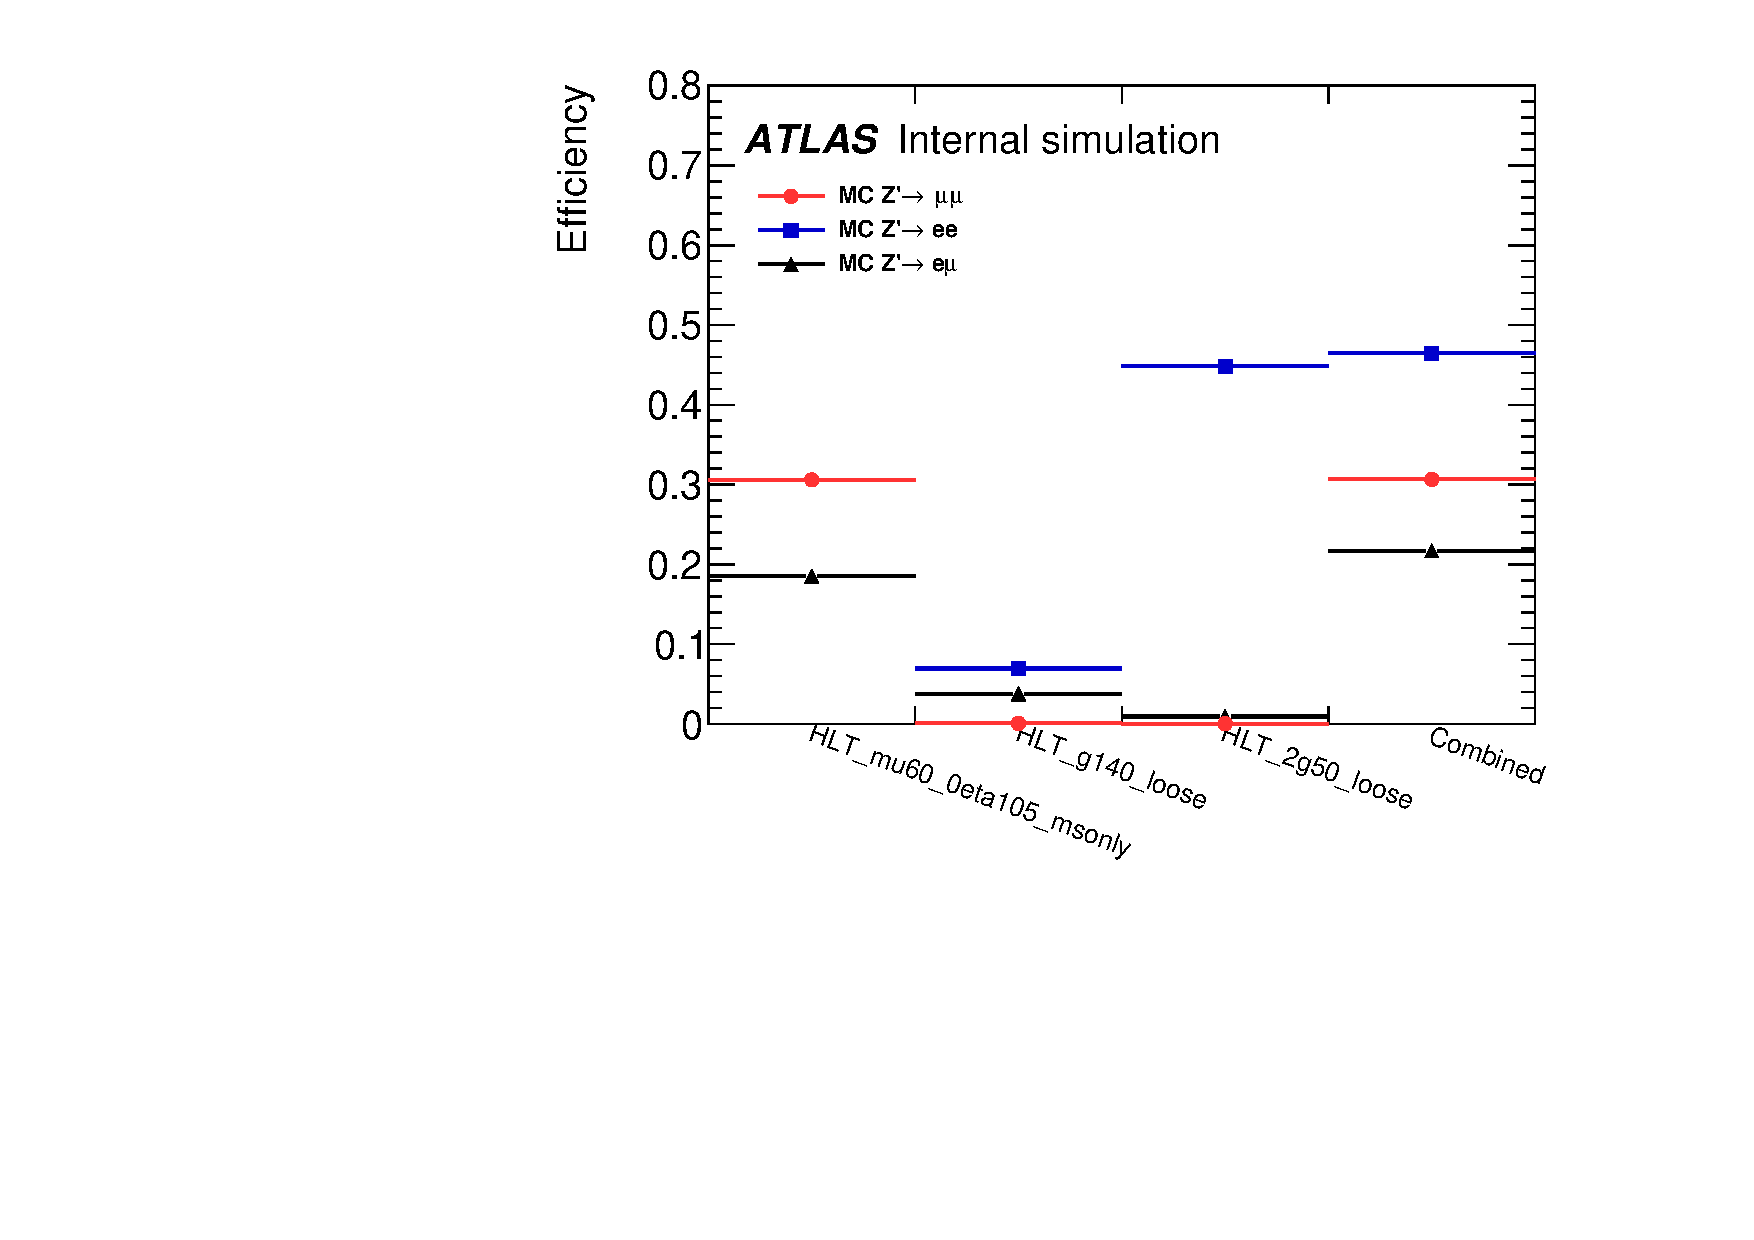
\includegraphics[width=0.60\textwidth]{figures/m_dv_eff_trig_allchannel.pdf}
	\centering
	\caption{Trigger efficiency of single muon, single photon, di-photon, and the combined triggers of the signal MC samples of $Z'\rightarrow\mumu, \ee$, and \emu generated with $m=$ 250 GeV and $c\tau=$ 250 mm.}
	\label{fig:m_trig_eff_allchannel}
\end{figure}

The trigger efficiency of all $Z'$ signal MC samples is shown in Appendix~\ref{app:trig_eff}. It is evident that at low $Z'$ mass ($\sim$100 GeV), the combined trigger efficiency of the signal MC sample is significantly reduced because typical $p_{T}$ of the signal leptons is lower than the $p_{T}$ threshold of the triggers.

The trigger study indicates that there is a substantial loss in the signal efficiency at trigger level before reconstruction, and developing dedicated, more efficient triggers for long-lived particles will provide potential improvement in sensitivity to long-lived particles. 


\subsection{Trigger Scale Factors}
\label{sec:syst:trigger}

The triggers may not be well simulated by the MC. Therefore, the trigger efficiency is estimated directly from the data using the \textit{tag--and--probe} method with $Z$+jet events. The estimated efficiency is compared with the trigger efficiency from the MC samples obtained using the same method. 

The tag--and--probe method uses $Z$ to two leptons (\ee and \mumu) final states, identified with one lepton passing tight requirement (\textit{tag}) and the other lepton passing loose requirement (\textit{probe}). The two-lepton invariant mass must be consistent with the $Z$ mass. The tag must satisfy the trigger requirement so that the fraction of the probes that satisfies the trigger requirement of interest is then the trigger efficiency.

Since the standard tag-and-probe method uses prompt $Z$+jet events, i.e. $Z$ decays at small impact parameters, this method can be used only if the trigger efficiency does not depend on the impact parameters. Figure~\ref{fig:signal_TrigEff} shows that both the photon and muon triggers have small dependence on the impact parameters since both triggers do not rely on inner detector information. The photon trigger efficiency is uniform up to $|\dzero| <$ 200 mm and $|\zzero| <$ 300 mm. The muon trigger efficiency starts to decrease for large impact parameters, $|\dzero| \sim120~\si{\mm}$ and $|\zzero| \sim200~\si{\mm}$. However, the decreasing muon efficiency at very large impact parameters is neglected since the fraction of reconstructed muons with such large impact parameters is less than 10\% at the lifetime of $c\tau=100~\si{\mm}$.


\begin{figure}[!htp]
    \centering
    \subfloat[]{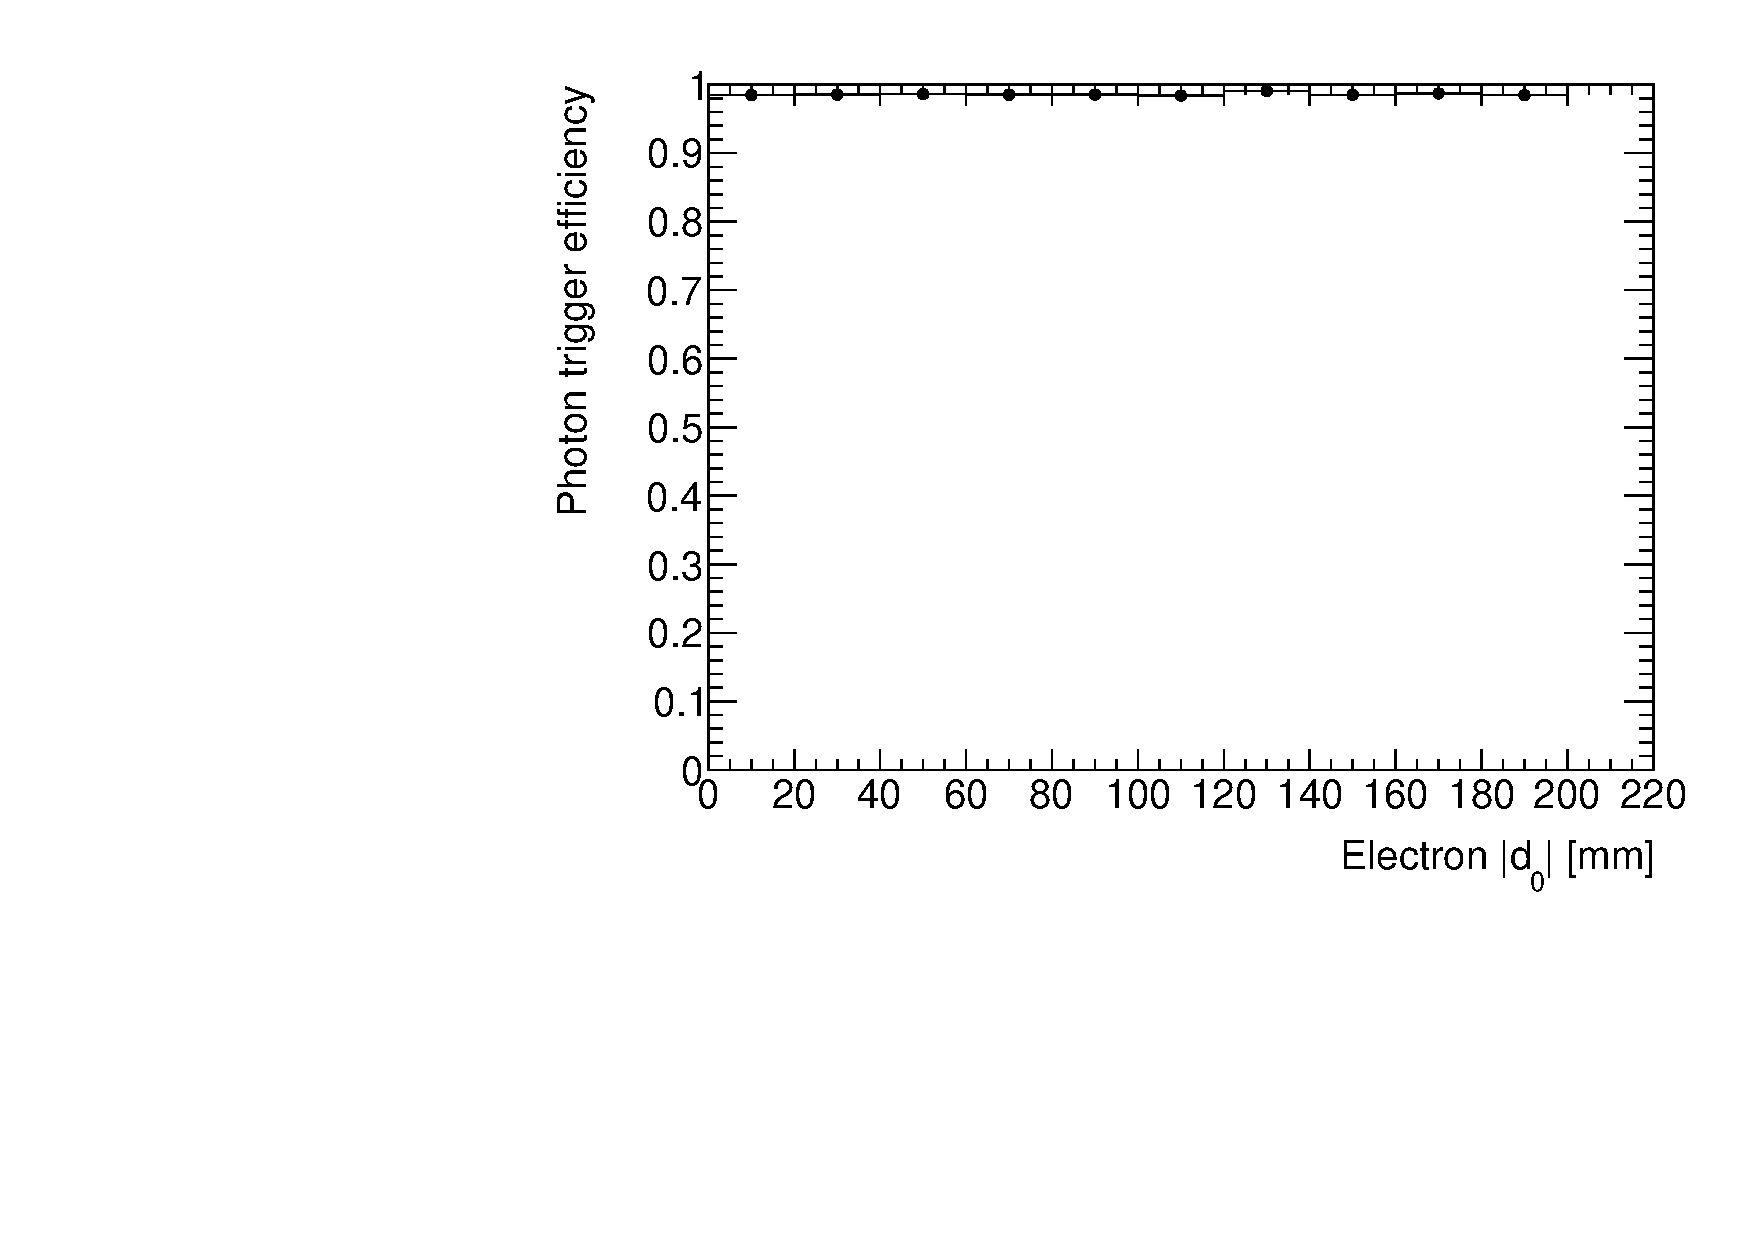
\includegraphics[width = 0.44 \textwidth]{figures/TrigEff/signal/eff_siph_d0.pdf}}
    \subfloat[]{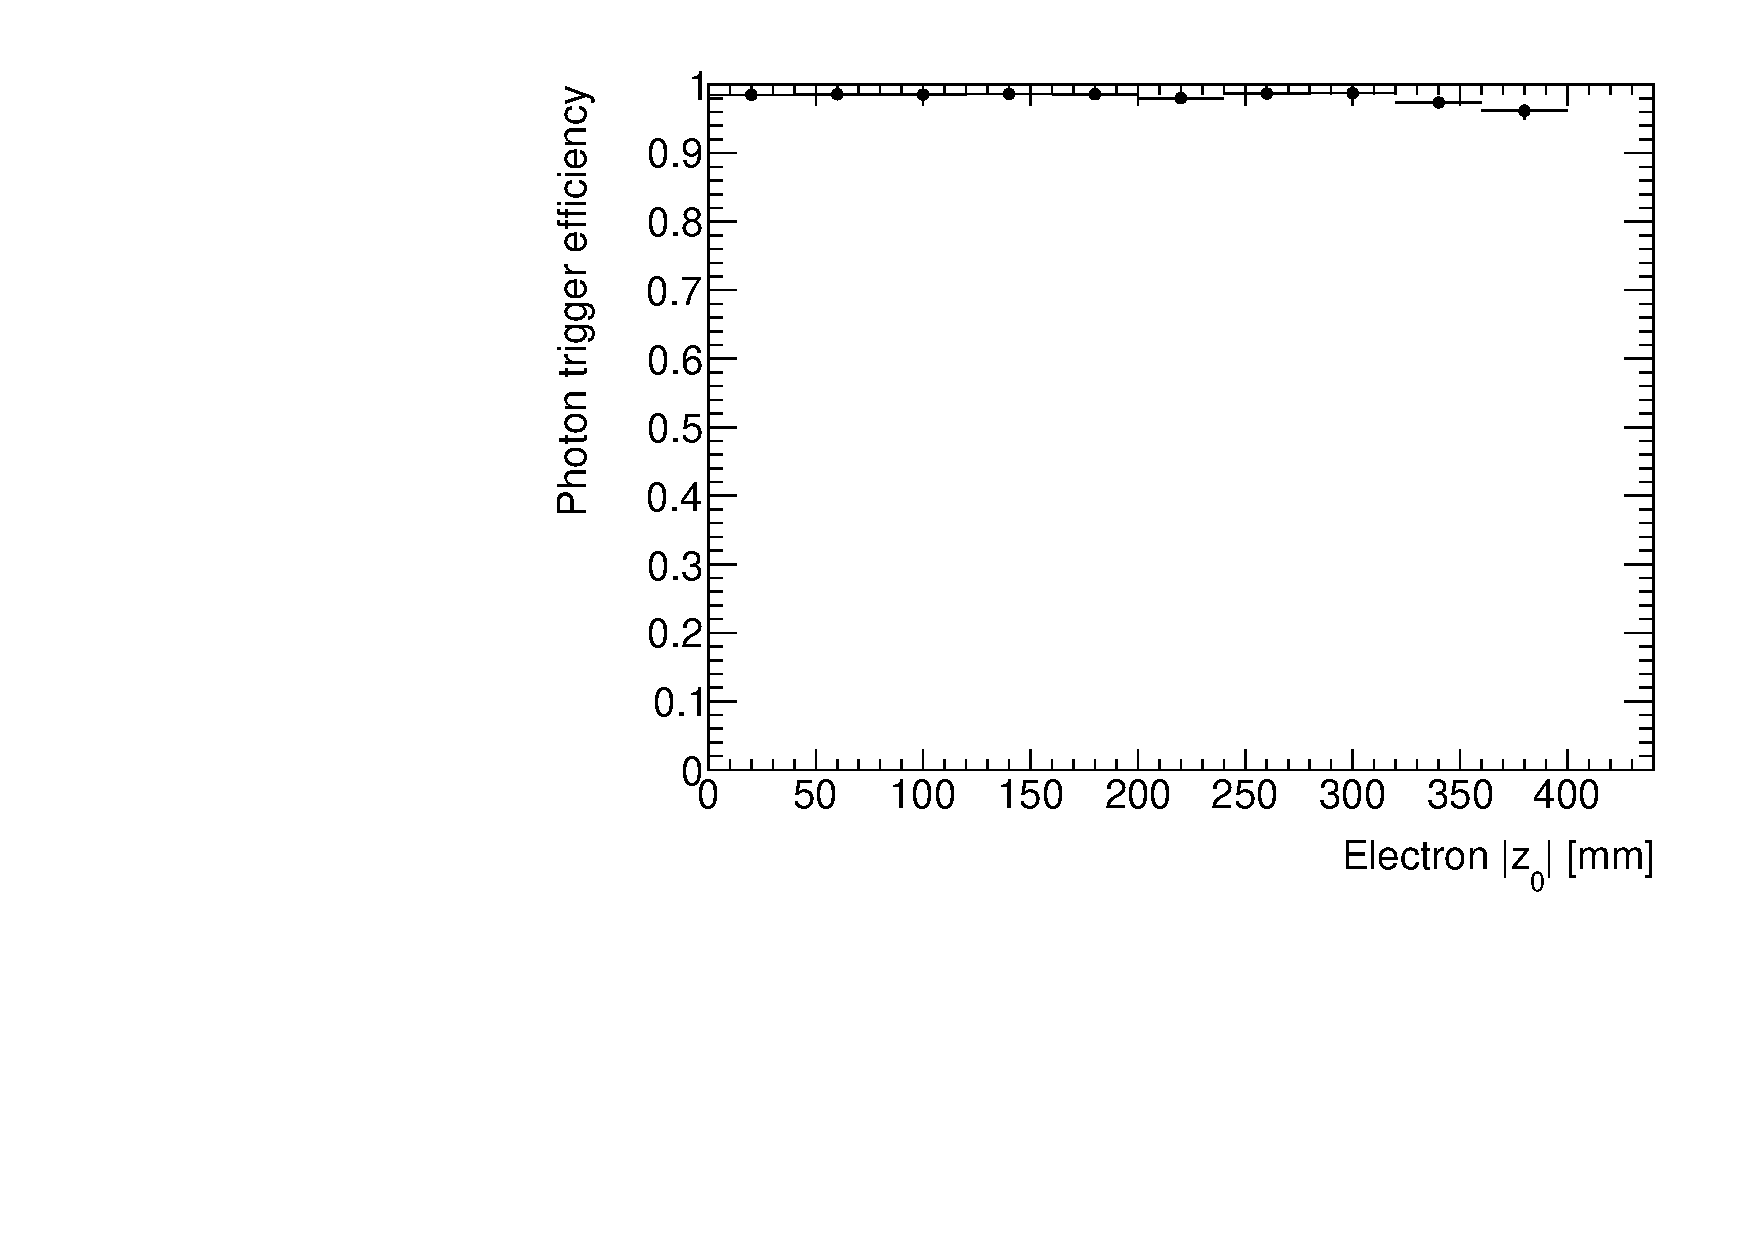
\includegraphics[width = 0.44 \textwidth]{figures/TrigEff/signal/eff_siph_z0.pdf}} \\
    \subfloat[]{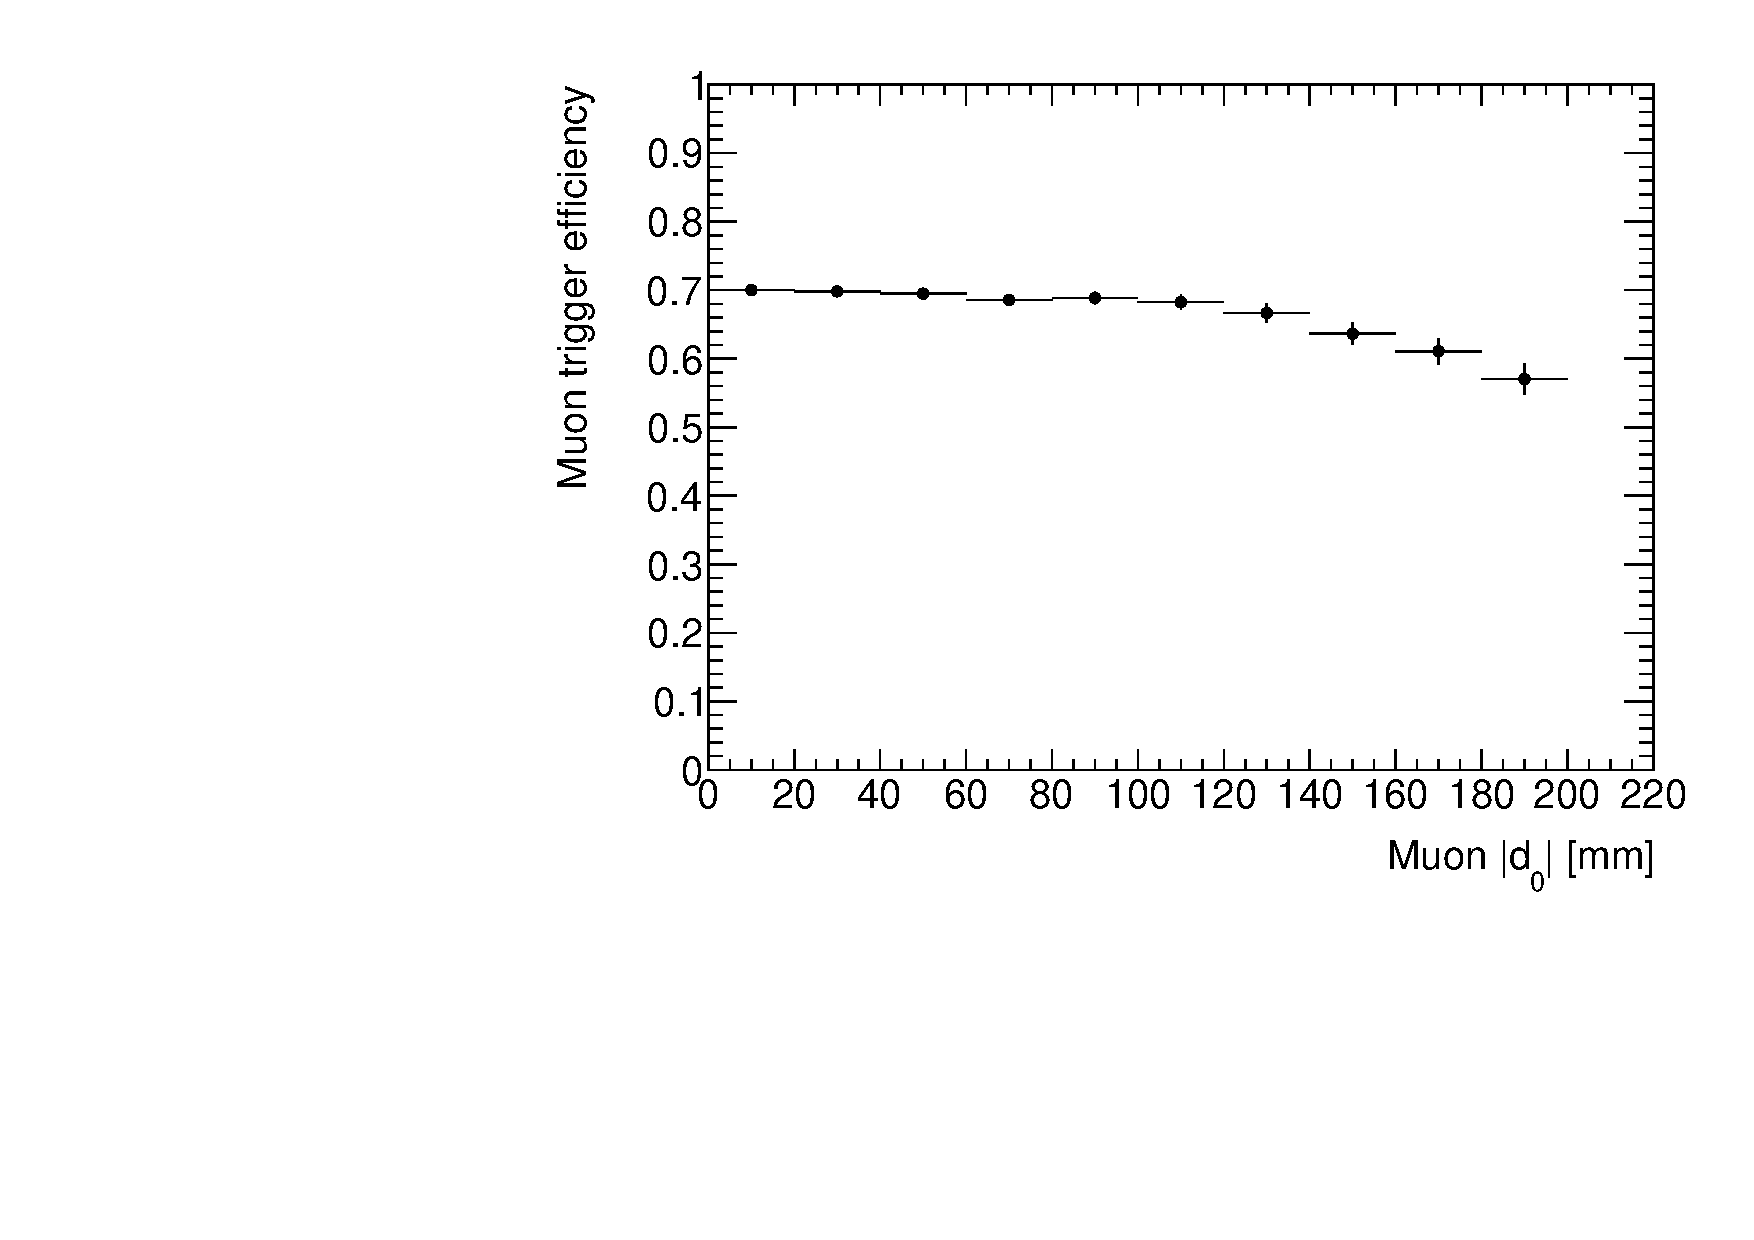
\includegraphics[width = 0.44 \textwidth]{figures/TrigEff/signal/eff_simu_d0.pdf}}
    \subfloat[]{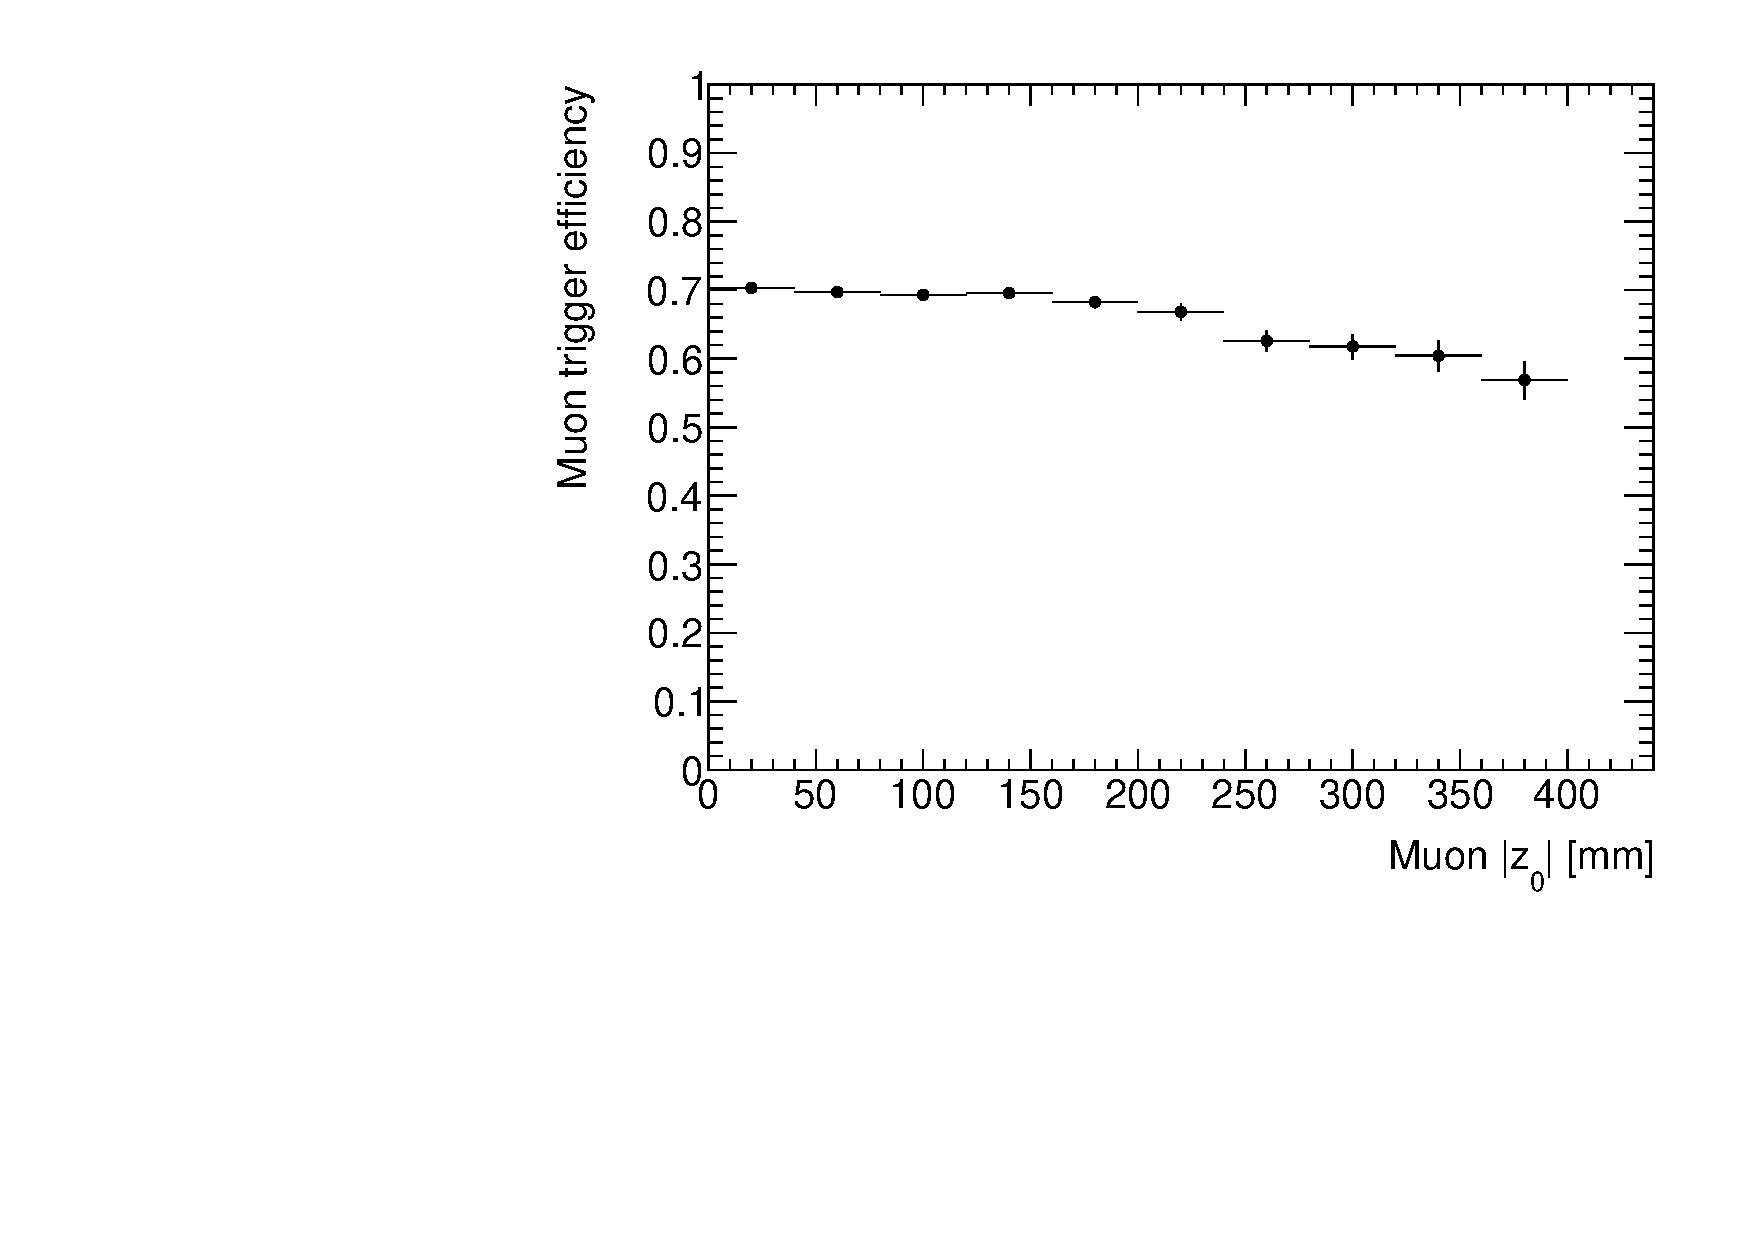
\includegraphics[width = 0.44 \textwidth]{figures/TrigEff/signal/eff_simu_z0.pdf}}
    \caption{The efficiency of the single photon trigger for an electron as a function of (a) $|\dzero|$ and (b) $|\zzero|$. The corresponding plots of the single muon trigger are shown in (c) and (d).}
    \label{fig:signal_TrigEff}
\end{figure}



\subsubsection{Photon Triggers}
\label{subsect:photonTrigEff}

The scale factors of the single photon and the di-photon triggers are estimated with a standard tag and probe method on $Z\rightarrow ee$ events by comparing the efficiency in data and MC samples. The di-photon trigger (\texttt{HLT\_2g50\_loose}) is studied using the single photon trigger (\texttt{HLT\_g50\_loose}) with the same $p_{T}$ threshold. The selection criteria of electron tag--and--probe candidates are listed in Table~\ref{tab:ZeeSelection}. In addition, pairs are required to have opposite signs and to satisfy the mass requirement ($|m_{e^{+}e^{-}} - m_{Z}| < 10~\si{\GeV}$) and the isolation requirement of $\DeltaR(\mathrm{tag}, \mathrm{probe}) > 0.4$. 

\begin{table}[!htb]
	\centering
	\begin{tabular}{ccc}
		\hline
		\hline
		Selection               & Tag                                           & Probe         \\
		\hline
		$p_{T}$ (GeV)           & $>$ 27                                        & $>$ 30        \\
		Trigger matched         & \texttt{HLT\_e26\_lhtight\_nod0\_ivarloose}   & -             \\
		$|\eta|$                & $<$ 1.37 or 1.52 - 2.47                       & $<$ 2.47      \\
		Identification          & TightLH                                       & LooseLHNoD0   \\
		Object quality          & yes                                           & yes           \\
		Track isolation         & yes                                           & -             \\
		Jet veto                & -                                             & yes           \\
		\hline
		\hline
	\end{tabular}
	\caption{Selection criteria for tag--and--probe electrons in $Z$+jets studies.}
	\label{tab:ZeeSelection}
\end{table}

The invariant mass distributions of the tag--and--probe pairs found in the data and the MC samples are shown in Figure~\ref{fig:PhotonTrigMass}. It is evident that the background is negligible, and the shapes of distributions are in good agreement with data and MC. Therefore, no background subtraction is performed in the calculation of the trigger efficiencies, 

\begin{equation}
	\label{eq:TrigEff}
    \epsilon_{\mathrm{trigger}} = \frac{\textrm{Number of probes matched to trigger}}{\textrm{Number of probes}}.
\end{equation}
%
\begin{figure}[!htb]
    \centering
    \subfloat[]{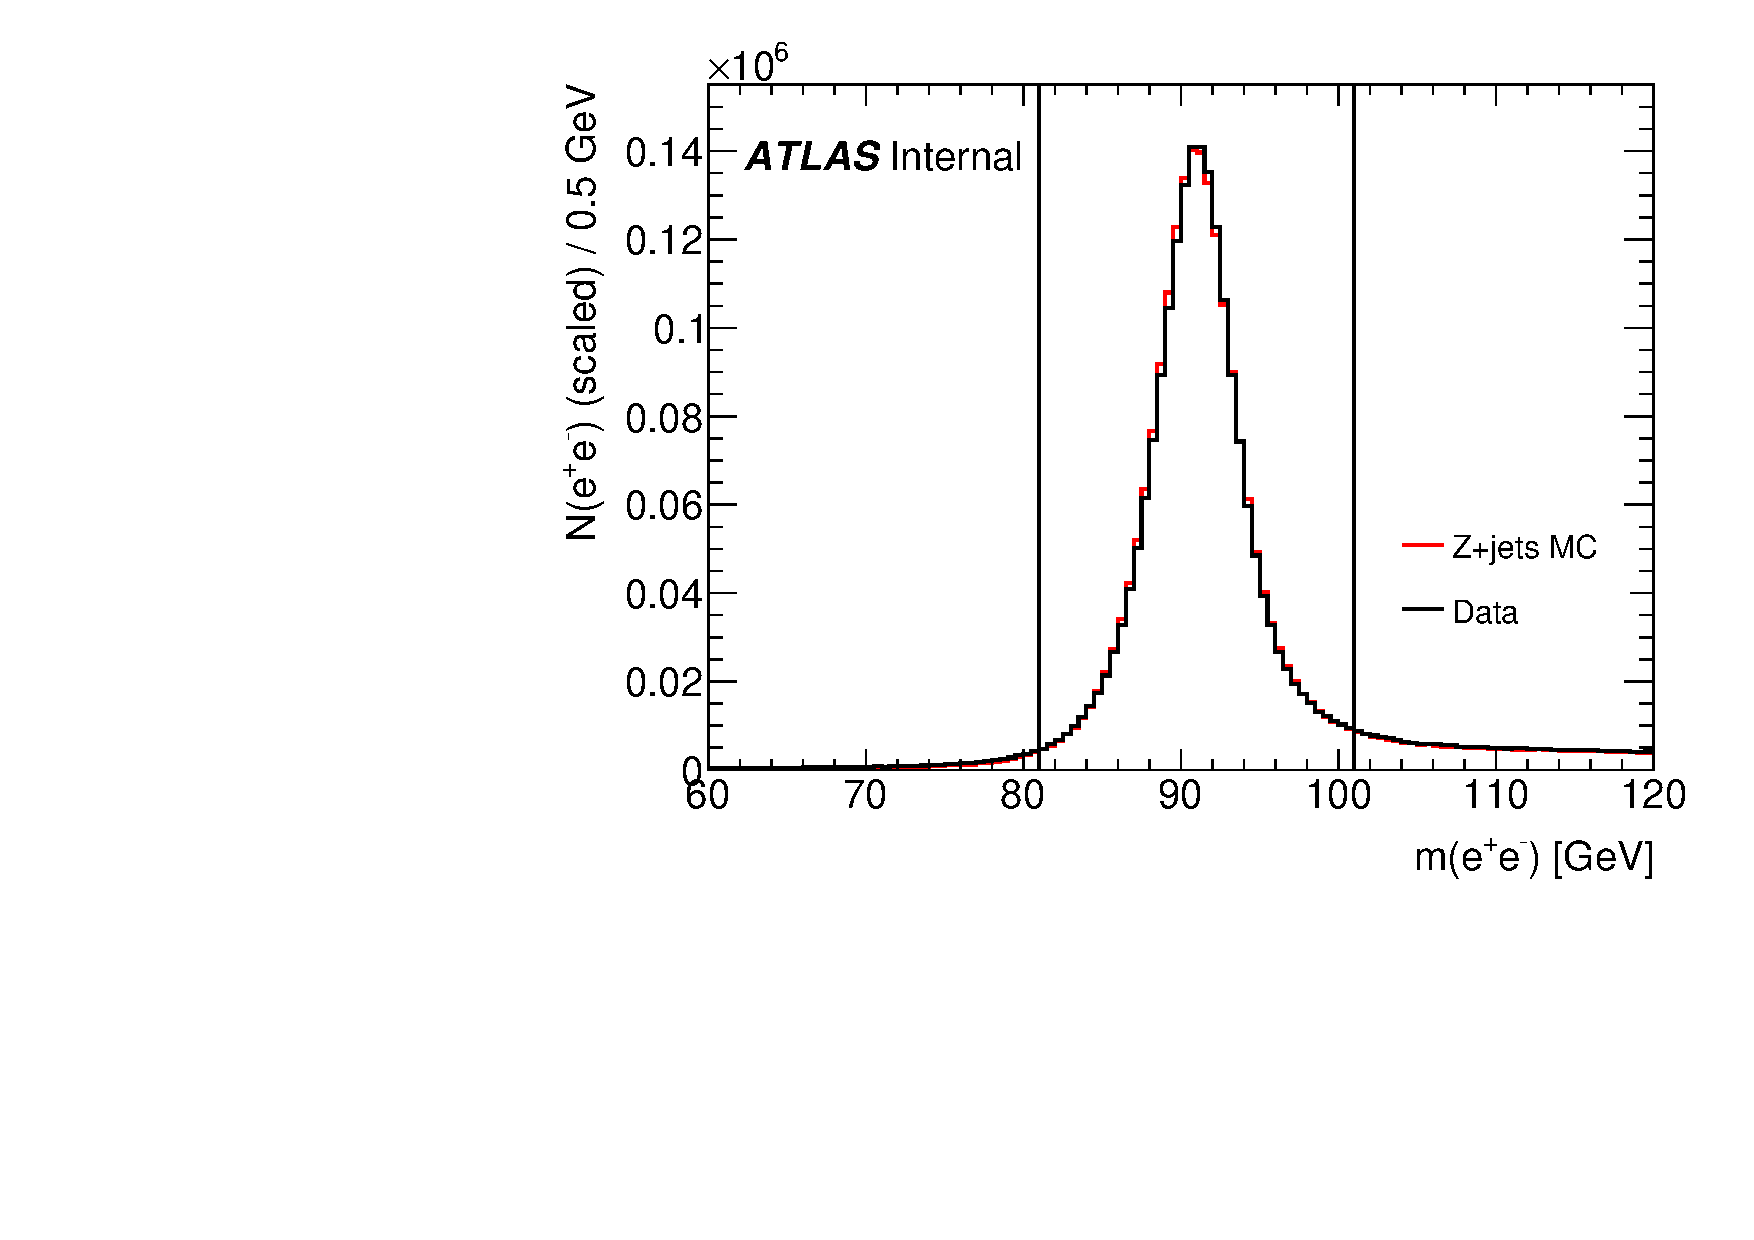
\includegraphics[width = 0.44 \textwidth]{figures/PhotonTrigEff/diph_mass.pdf}}
    \subfloat[]{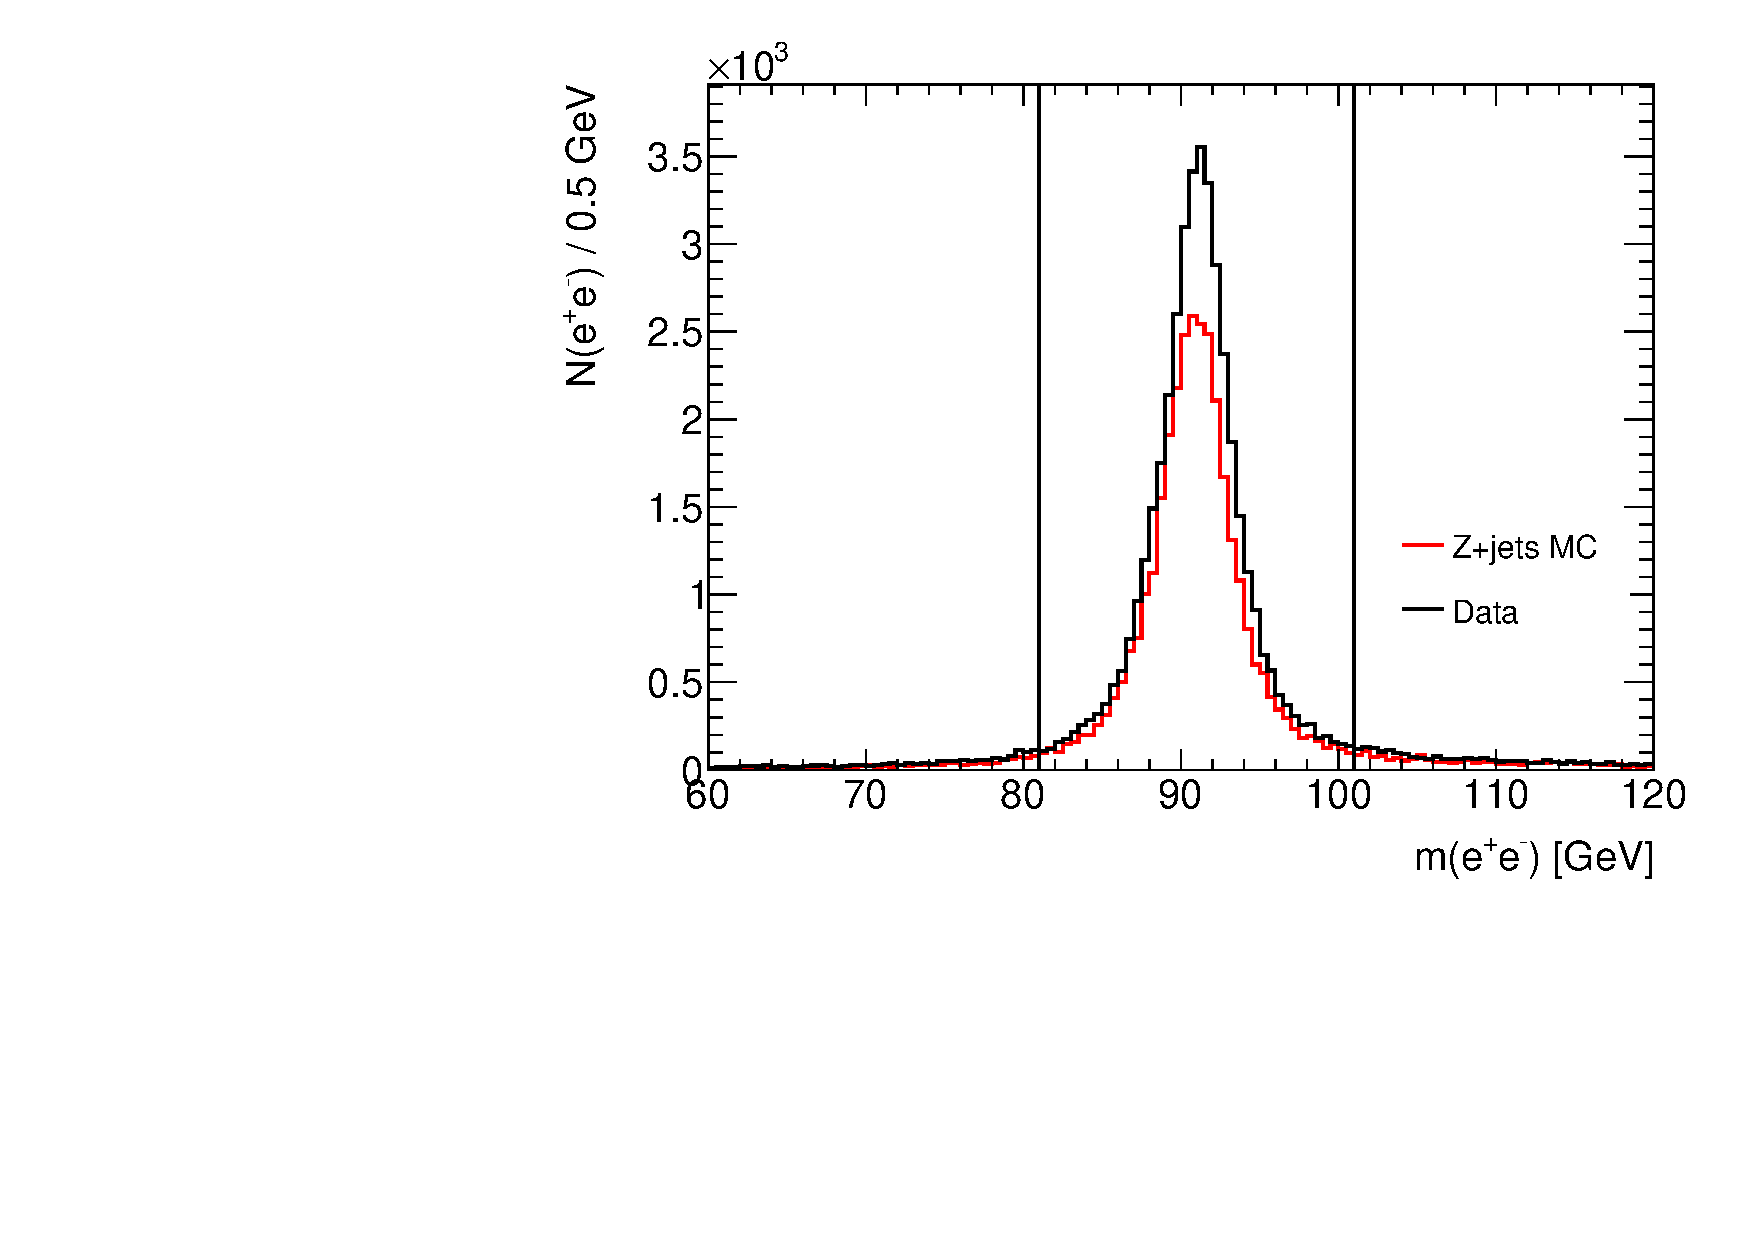
\includegraphics[width = 0.44 \textwidth]{figures/PhotonTrigEff/siph_mass.pdf}}
    \caption{Invariant mass distributions of the tag--and--probe electron pairs used to study the efficiencies of the (a) \texttt{HLT\_g50\_loose} and (b) \texttt{HLT\_g140\_loose} trigger in the data and $Z$+jets MC samples. The vertical lines indicate the mass window of the $Z$ candidates.
    }
    \label{fig:PhotonTrigMass}
\end{figure}

The selected tag--and--probe electrons are used to estimate the efficiencies of photon triggers, shown as a function of probe $p_{T}$, $\eta$, and $|\zzero|$ in Figure~\ref{fig:PhotonTrigEff}. The efficiency in $p_{T}$ shows that the \texttt{HLT\_g50\_loose} plateau starts at $55~\si{\GeV}$, and \texttt{HLT\_g140\_loose} plateau starts at $148~\si{\GeV}$, and the electrons in this plateau region are used to estimate the trigger efficieny in Fig.~\ref{fig:PhotonTrigEff}(c-f). The efficiency in $\eta$ shows good agreement between data and MC for electrons reconstructed inside the barrel, whereas a small discrepancy in efficiency is shown for electrons at the boundary regions and in the end-cap regions. Also, the efficiency in $|\zzero|$ shows no dependence of the photon trigger efficiencies on $|\zzero|$.

The ratio of the efficiency from data to MC, binned in $\eta$, is taken as a scale factor and applied to the efficiency calculation.



\begin{figure}[!htb]
    \centering
    \subfloat[]{\label{fig:PhotonTrigEff:di_pt}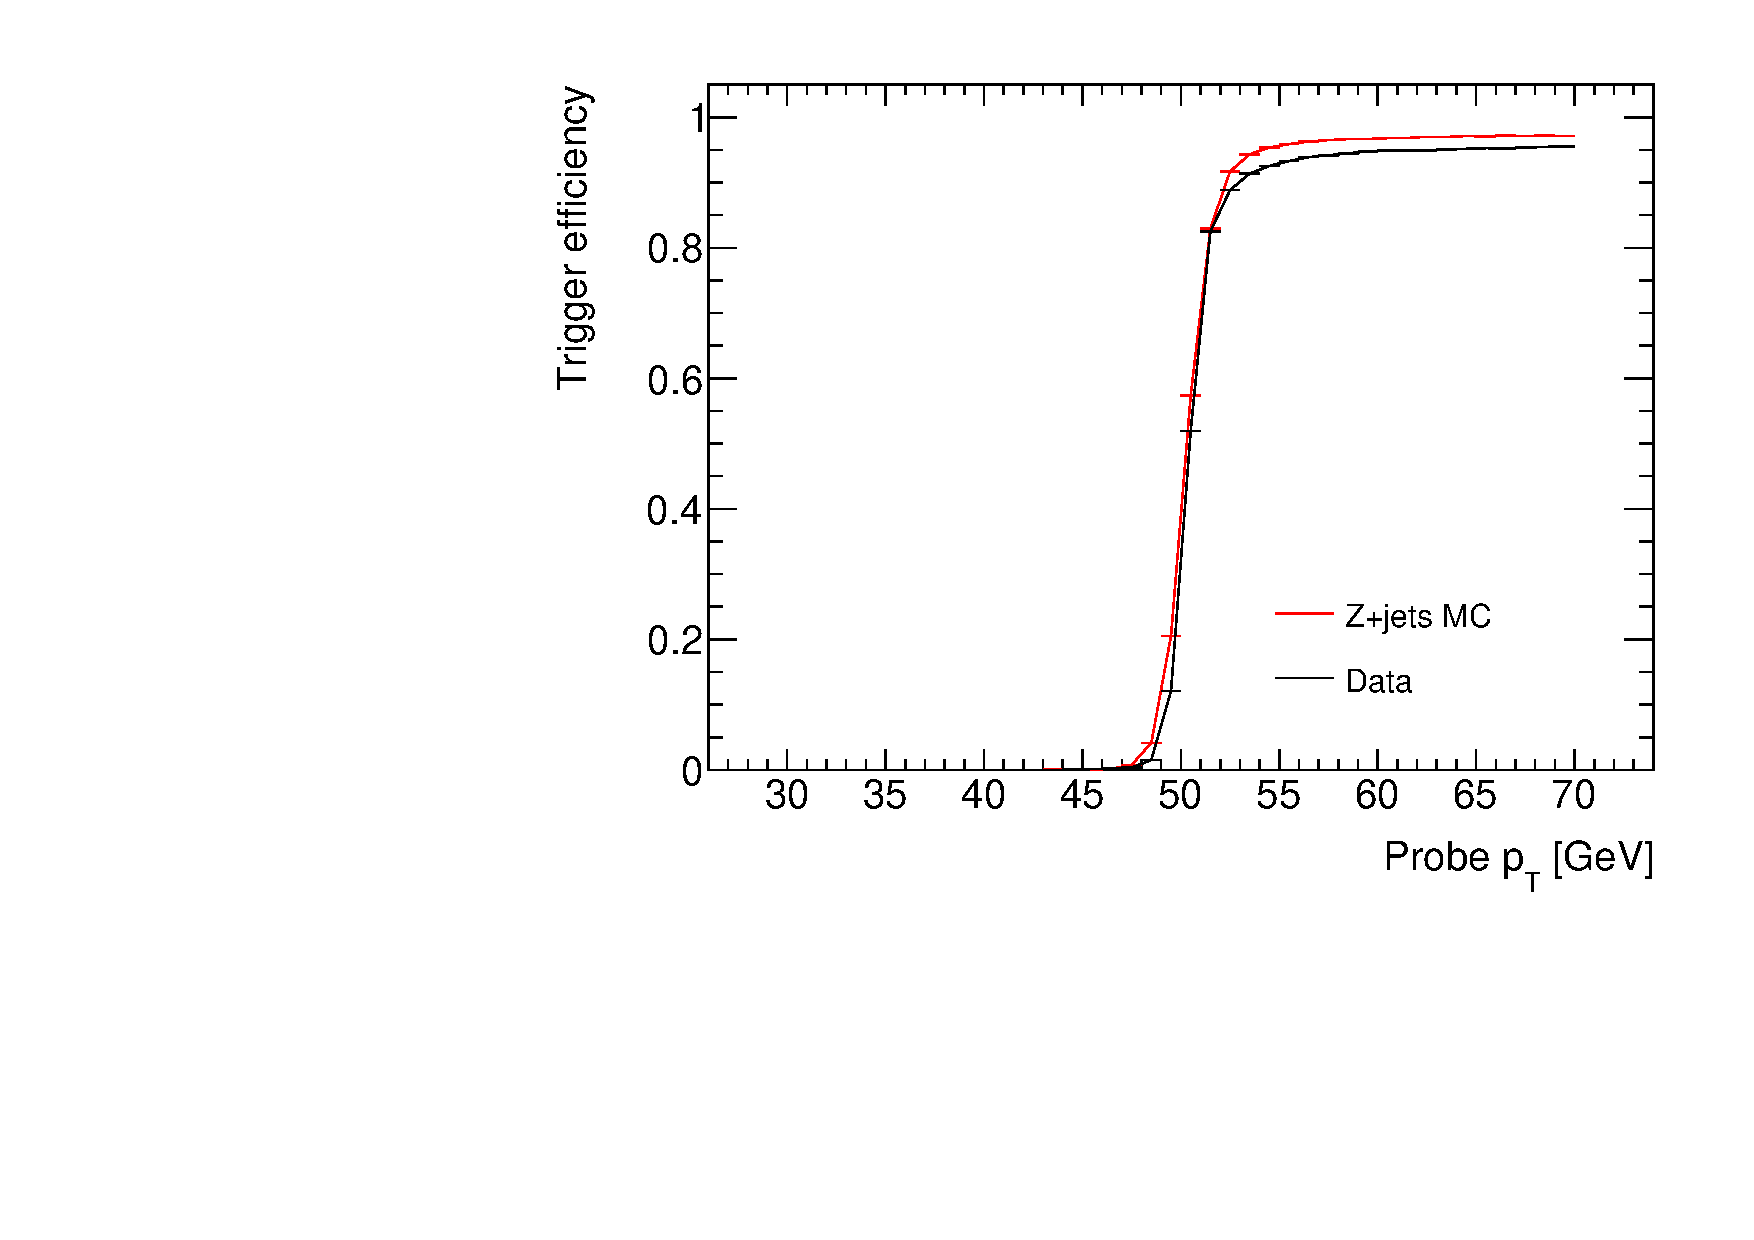
\includegraphics[width = 0.44 \textwidth]{figures/PhotonTrigEff/diph_eff_pt.pdf}}
    \subfloat[]{\label{fig:PhotonTrigEff:si_pt}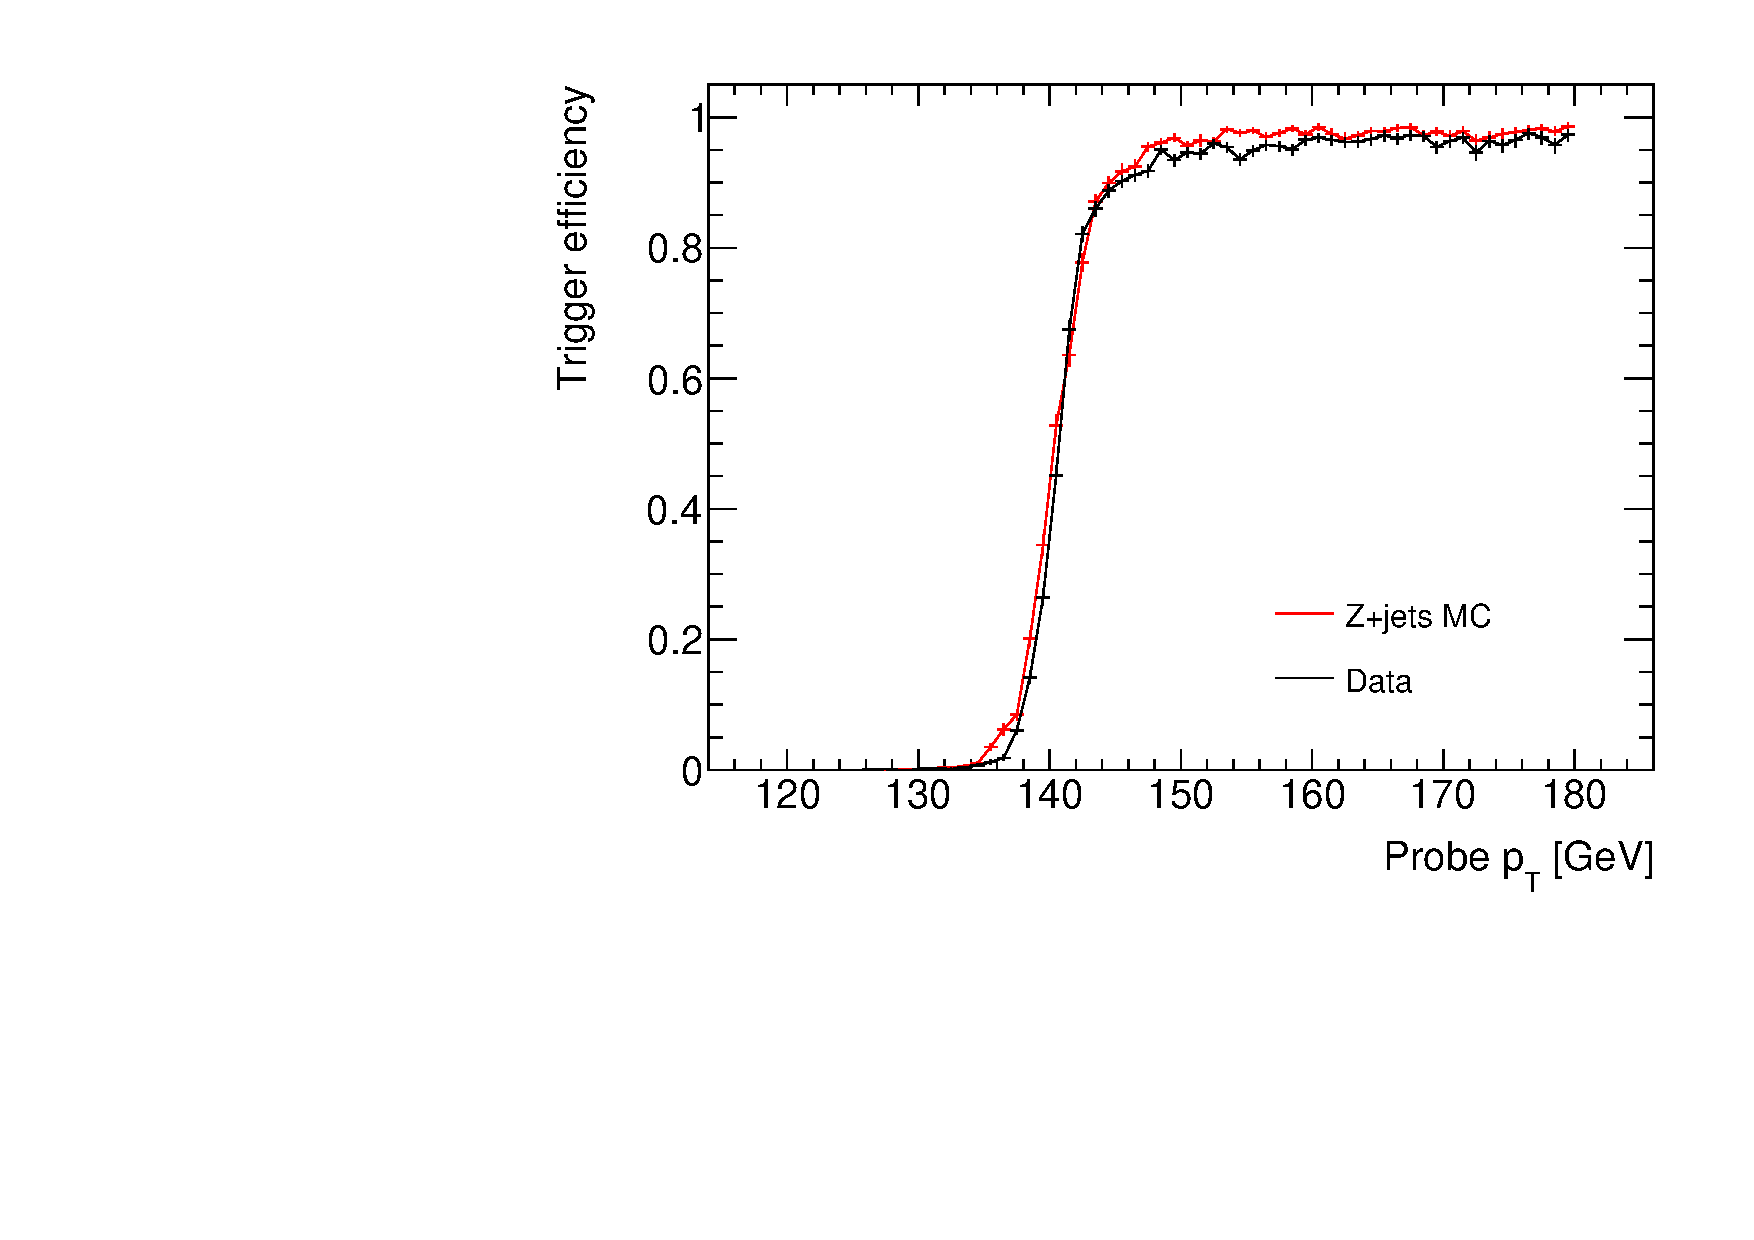
\includegraphics[width = 0.44 \textwidth]{figures/PhotonTrigEff/siph_eff_pt.pdf}} \\
    \subfloat[]{\label{fig:PhotonTrigEff:di_eta}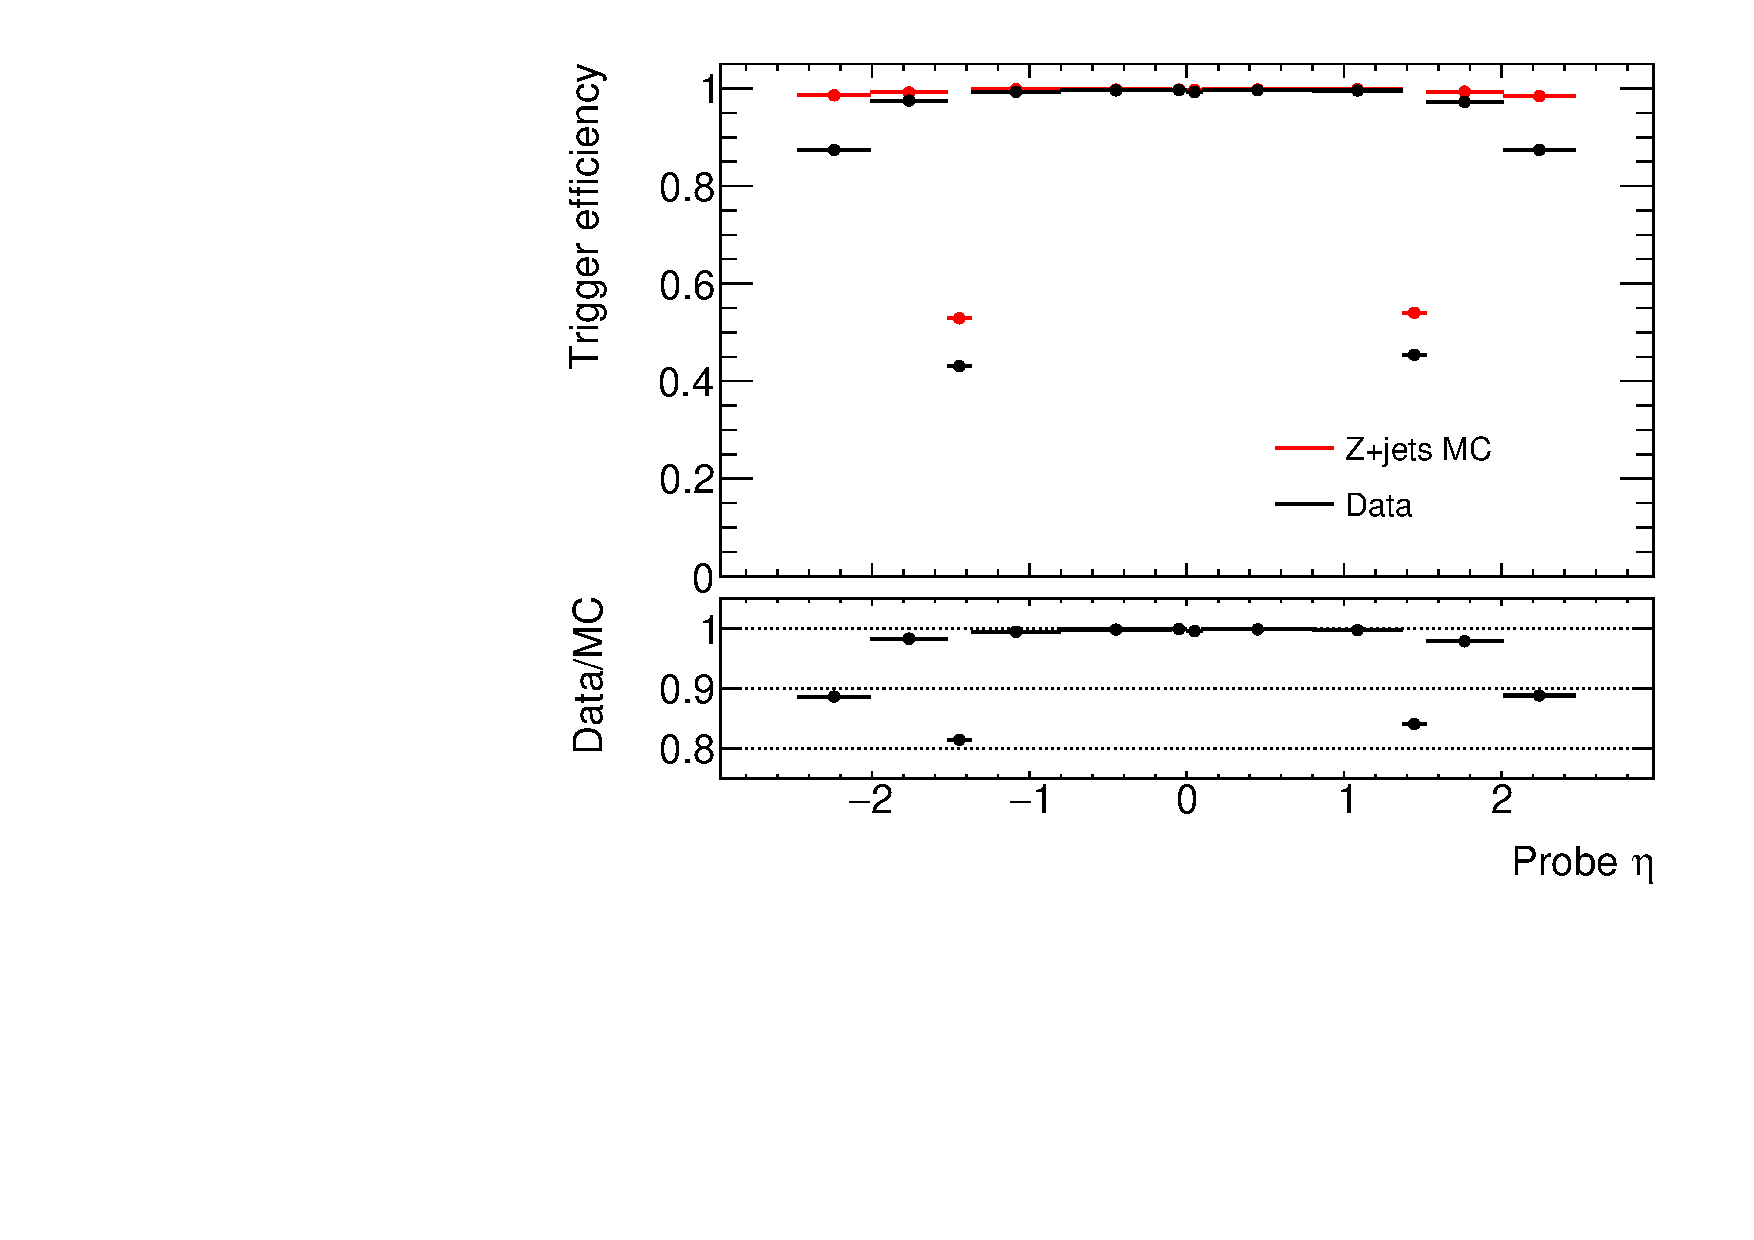
\includegraphics[width = 0.44 \textwidth]{figures/PhotonTrigEff/diph_eff_eta.pdf}}
    \subfloat[]{\label{fig:PhotonTrigEff:si_eta}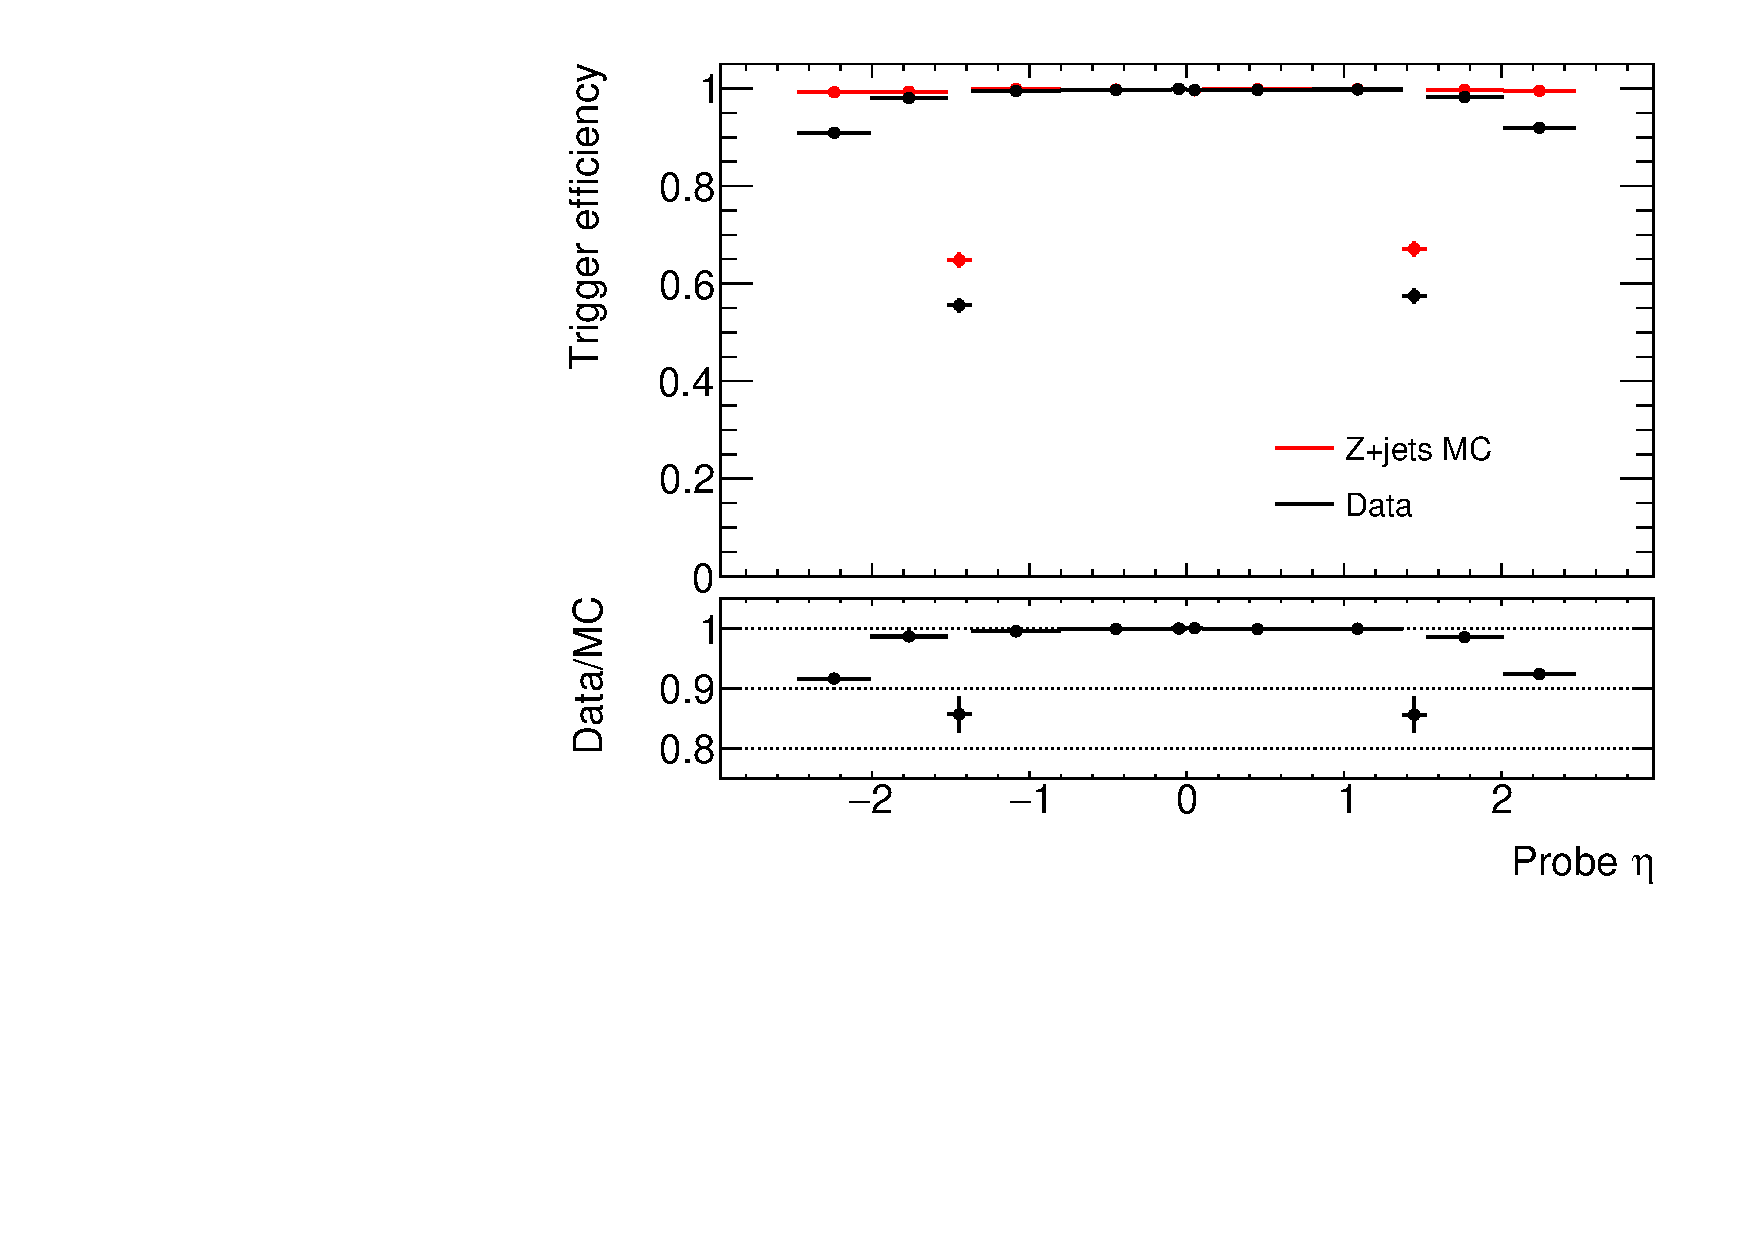
\includegraphics[width = 0.44 \textwidth]{figures/PhotonTrigEff/siph_eff_eta.pdf}} \\
    \subfloat[]{\label{fig:PhotonTrigEff:di_z0}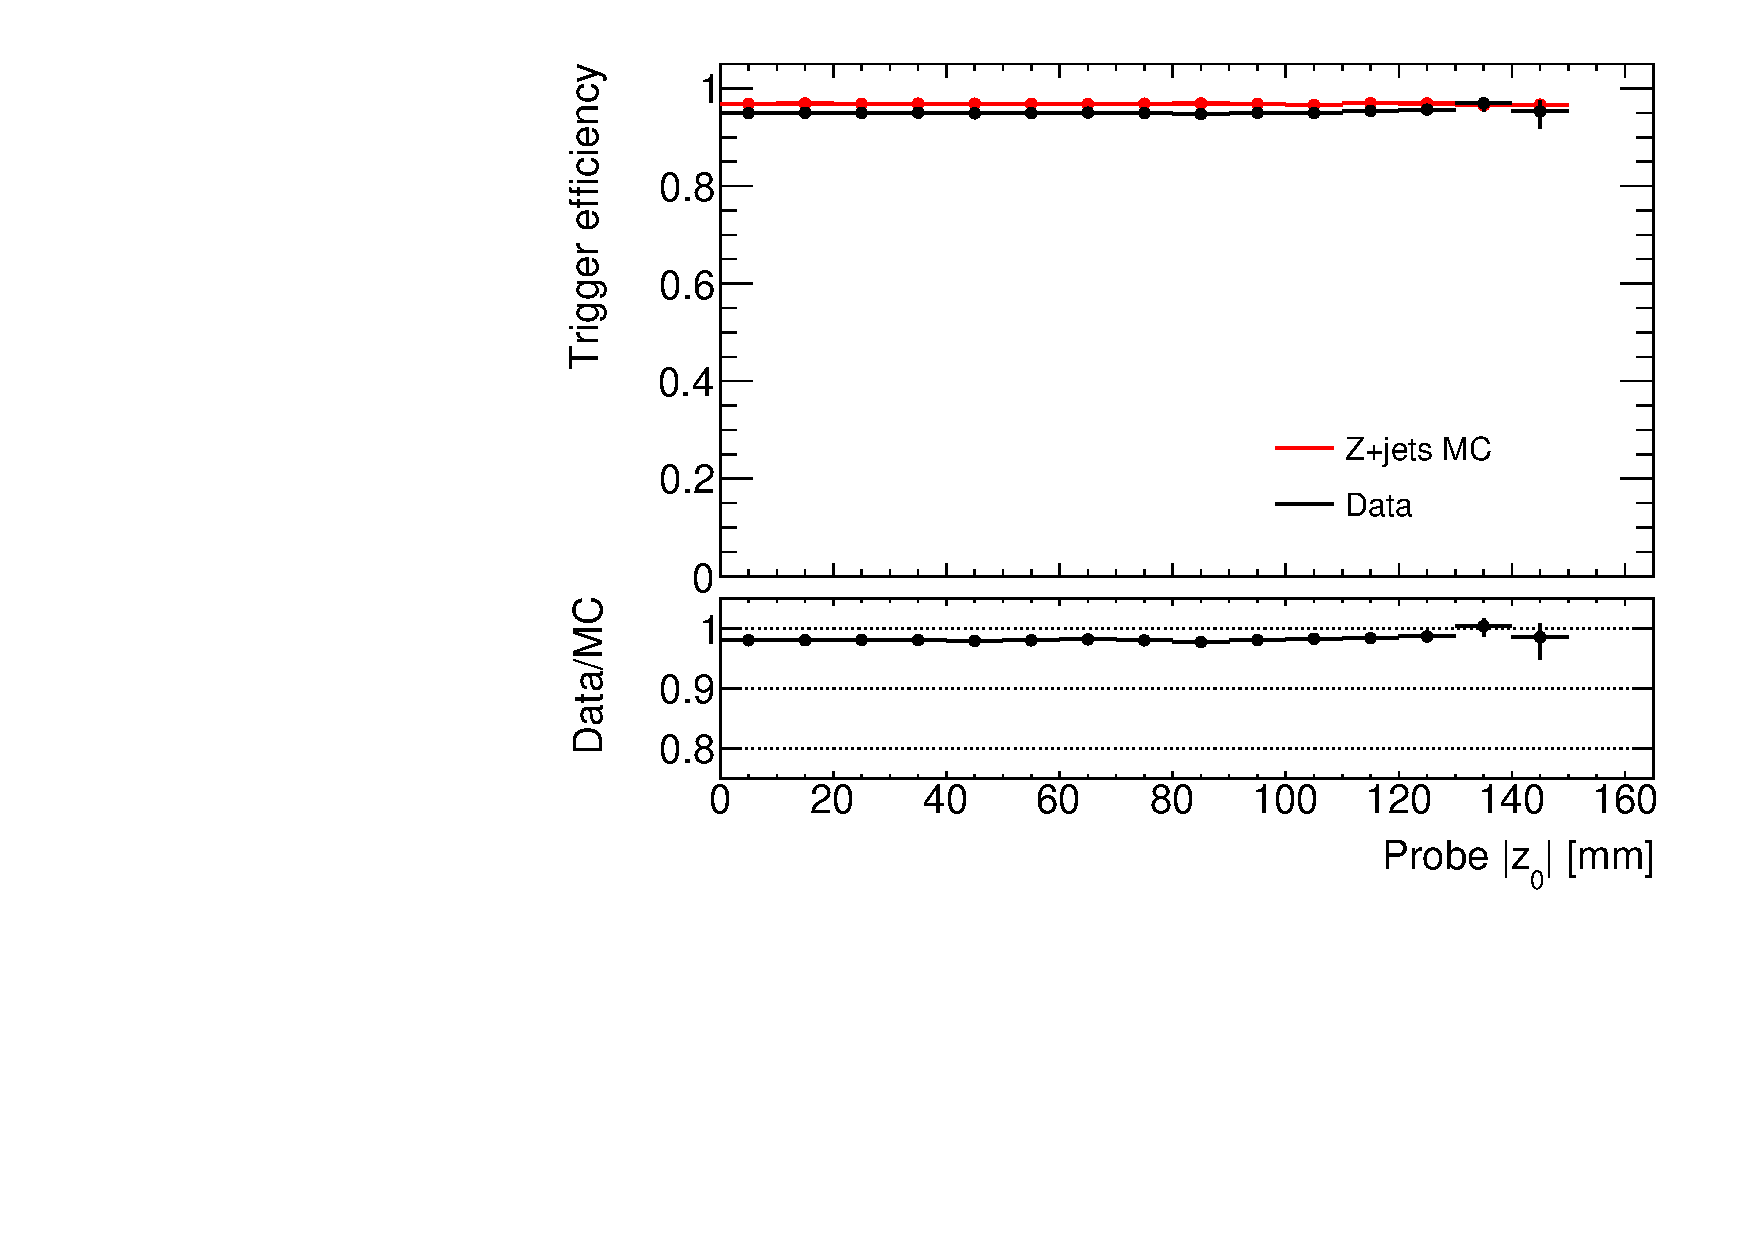
\includegraphics[width = 0.44 \textwidth]{figures/PhotonTrigEff/diph_eff_z0.pdf}}
    \subfloat[]{\label{fig:PhotonTrigEff:si_z0}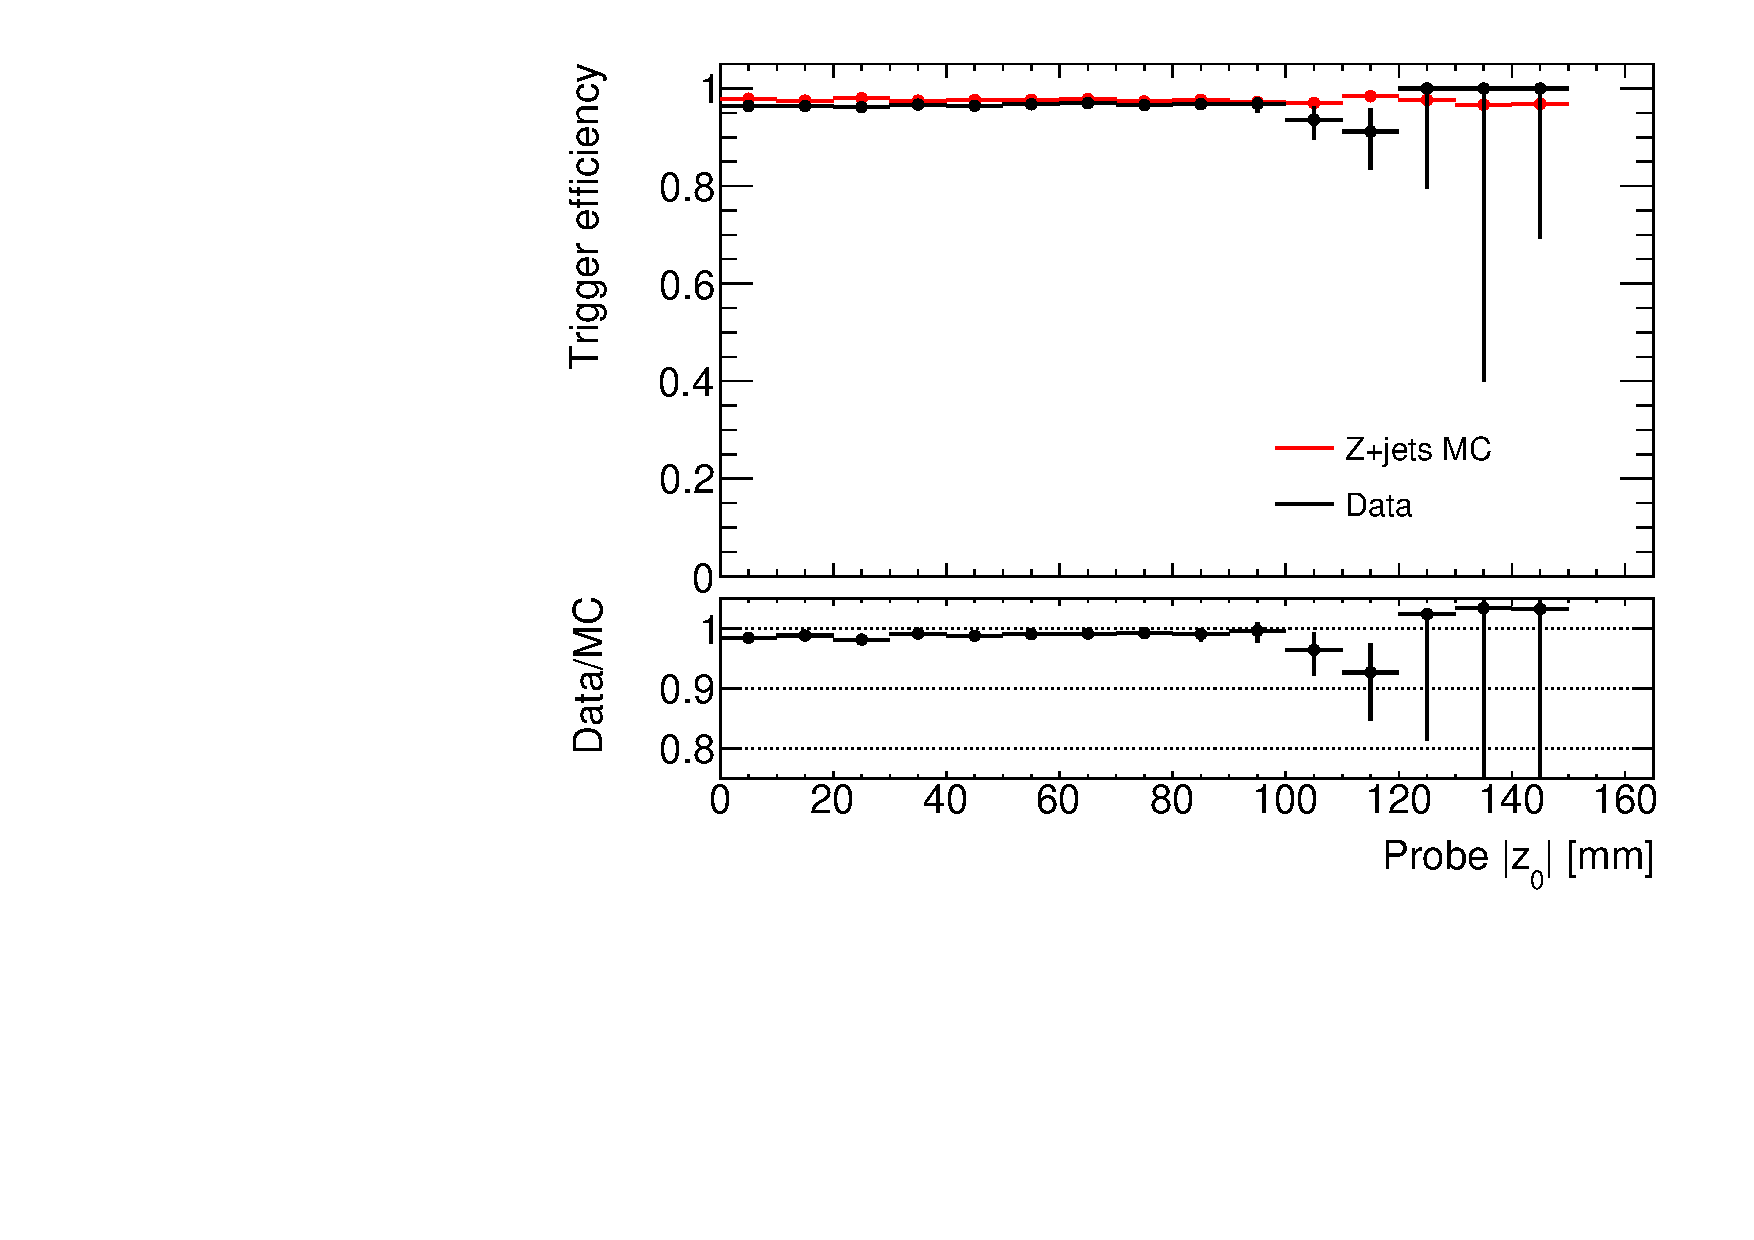
\includegraphics[width = 0.44 \textwidth]{figures/PhotonTrigEff/siph_eff_z0.pdf}}
    \caption{Efficiency of the \texttt{HLT\_g50\_loose} as a function of the (a) $p_{T}$, (c) $\eta$, and (e) $|\zzero|$ of the probe in the data and $Z$+jets MC samples. The corresponding plots of the \texttt{HLT\_g140\_loose} trigger are shown in (b), (d), and (f).
    }
    \label{fig:PhotonTrigEff}
\end{figure}




\subsubsection{Muon Trigger}
\label{subsect:muonTrigEff}

The scale factor of the single muon trigger is estimated with a standard tag--and--probe method on $Z \rightarrow \mu\mu$ events by comparing the efficiency in data and MC. The selection criteria of muon tag--and--probe candidates are listed in Table~\ref{tab:ZmmSelection}. Similar to the photon triggers, pairs are required to have opposite signs and to satisfy the mass requirement ($|m_{e^{+}e^{-}} - m_{Z}| < 10~\si{\GeV}$) and the isolation requirement of $\DeltaR(\mathrm{tag}, \mathrm{probe}) > 0.4$. 

\begin{table}[!htb]
	\centering
	\begin{tabular}{ccc}
		\hline
		\hline
		Selection           & Tag                               & Probe                     \\
		\hline
		$p_{T}$ (GeV)       & $>$ 28                            & $>$ 30                    \\
		Trigger matched     & \texttt{HLT\_mu26\_ivarmedium}    & -                         \\
		$|\eta|$            & $<$ 2.4                           & $<$ 1.05                  \\
		Identification      & Medium                            & Loose and combined        \\
		Isolation           & Loose                             & -                         \\
		\dzero significance & $< 3$                             & -                         \\
		$|\Delta \zzero \sin{\theta}|$ & $< 0.5~\si{\mm}$       & -                         \\
		\hline
		\hline
	\end{tabular}
	\caption{Selection criteria for tag--and--probe muons.}
	\label{tab:ZmmSelection}
\end{table}

The invariant mass distributions of the muon tag--and--probe pairs found in the data and the MC samples are shown in Figure~\ref{fig:MuonTrigMass}. It is evident that the background is negligible and therefore not corrected in calculating the trigger efficiency.

\begin{figure}[!htb]
    \centering
    \subfloat{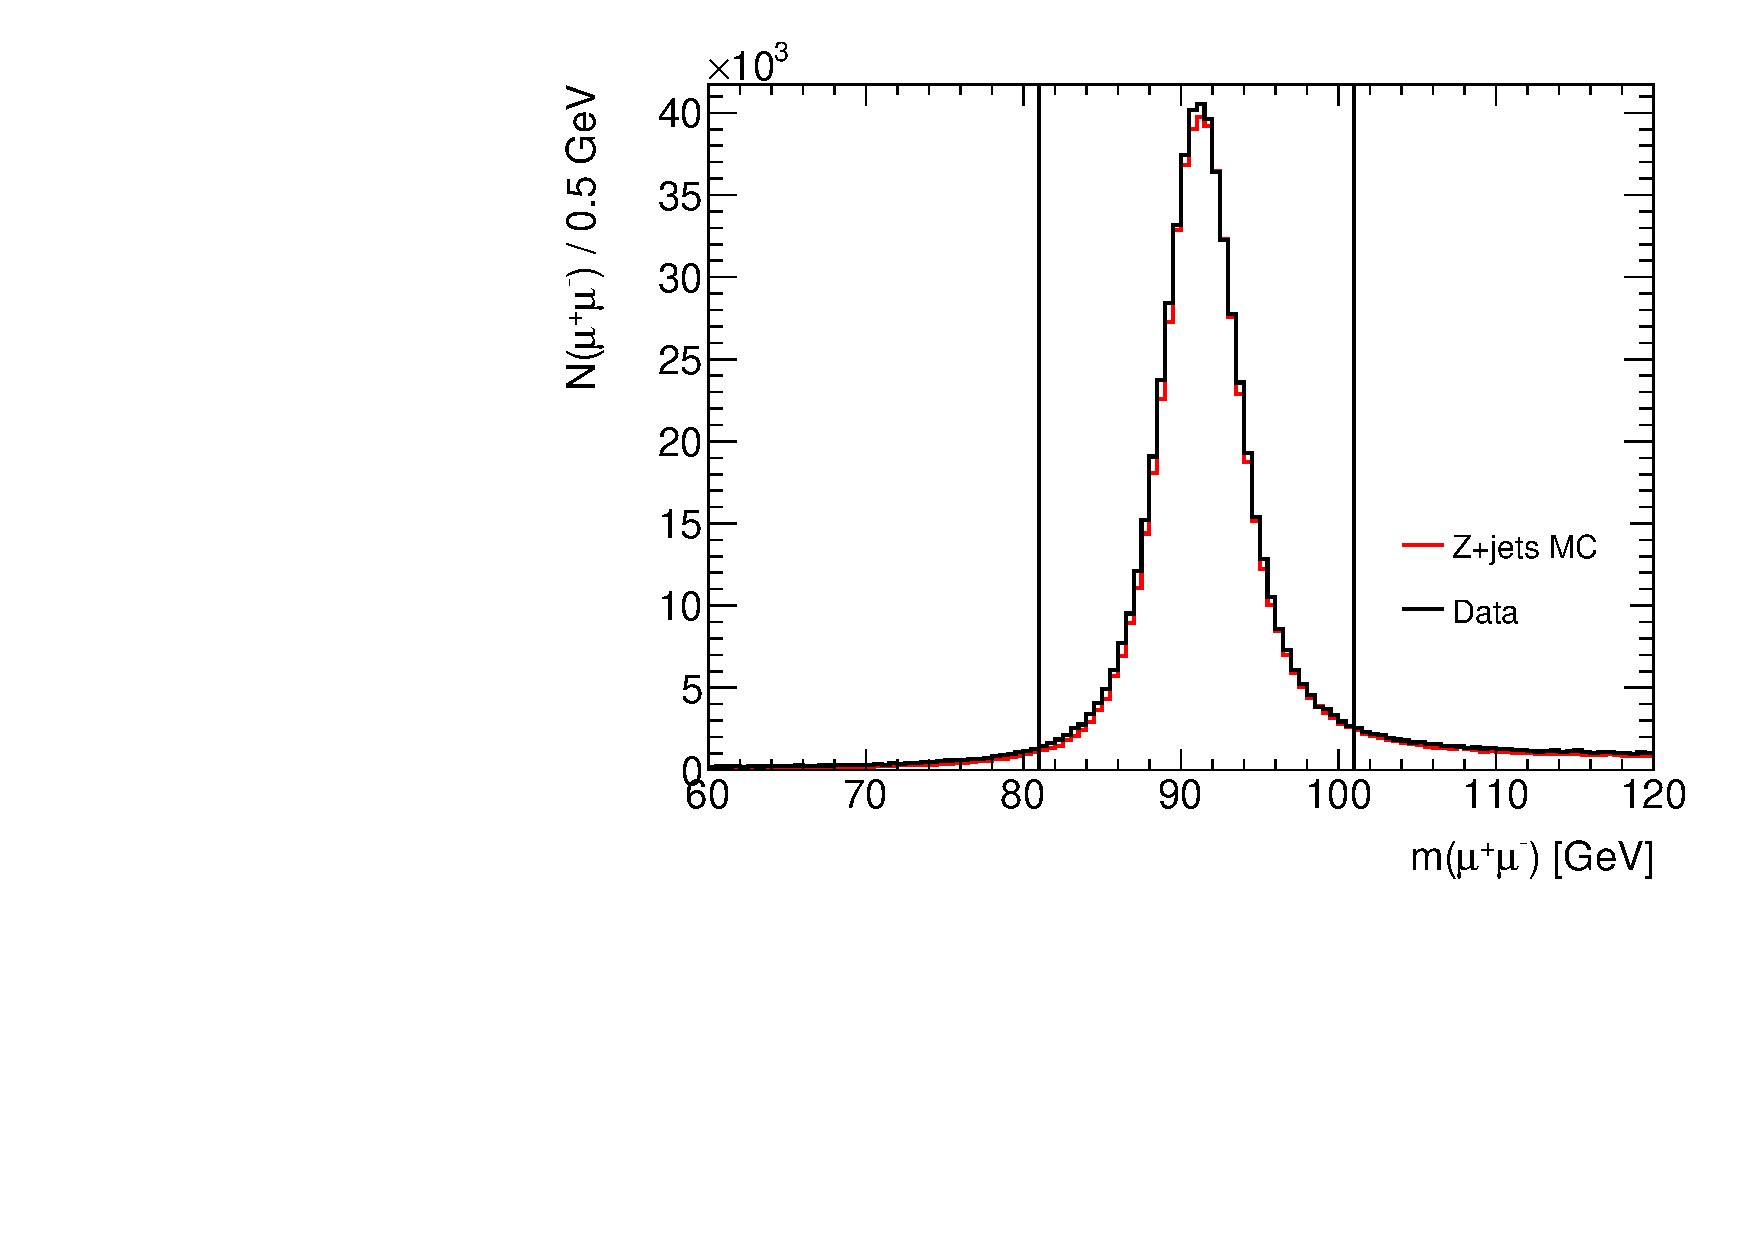
\includegraphics[width = 0.44 \textwidth]{figures/MuonTrigEff/mass.pdf}}
    \caption{Invariant mass distributions of the tag--and--probe muon pairs used to study the efficiencies of the single muon trigger in the data and $Z$+jets MC samples. The vertical lines indicate the mass window of the $Z$ candidates.
    }
    \label{fig:MuonTrigMass}
\end{figure}

The selected tag--and--probe muons are used to estimate the efficiency of the single muon trigger, shown as a function of probe $p_{T}$ and $|\zzero|$ in Figure~\ref{fig:MuonTrigEff1D}. The efficiency in $p_{T}$ shows that the efficiency plateau starts at $62~\si{\GeV}$. The efficiency is uniform up to $|\zzero|\sim$ 150 mm. In Figure~\ref{fig:MuonTrigEff2D}, the muons in this plateau region are used to compare the efficiency in data and MC. It is evident that efficiency depends on both $\phi$ and $\eta$. 

The ratio of the efficiency from data to MC, binned in $\phi$ and $\eta$, is taken as a scale factor and applied to the efficiency calculation.


\begin{figure}[!htb]
    \centering
    \subfloat[\label{fig:MuonTrigEff1Da}]{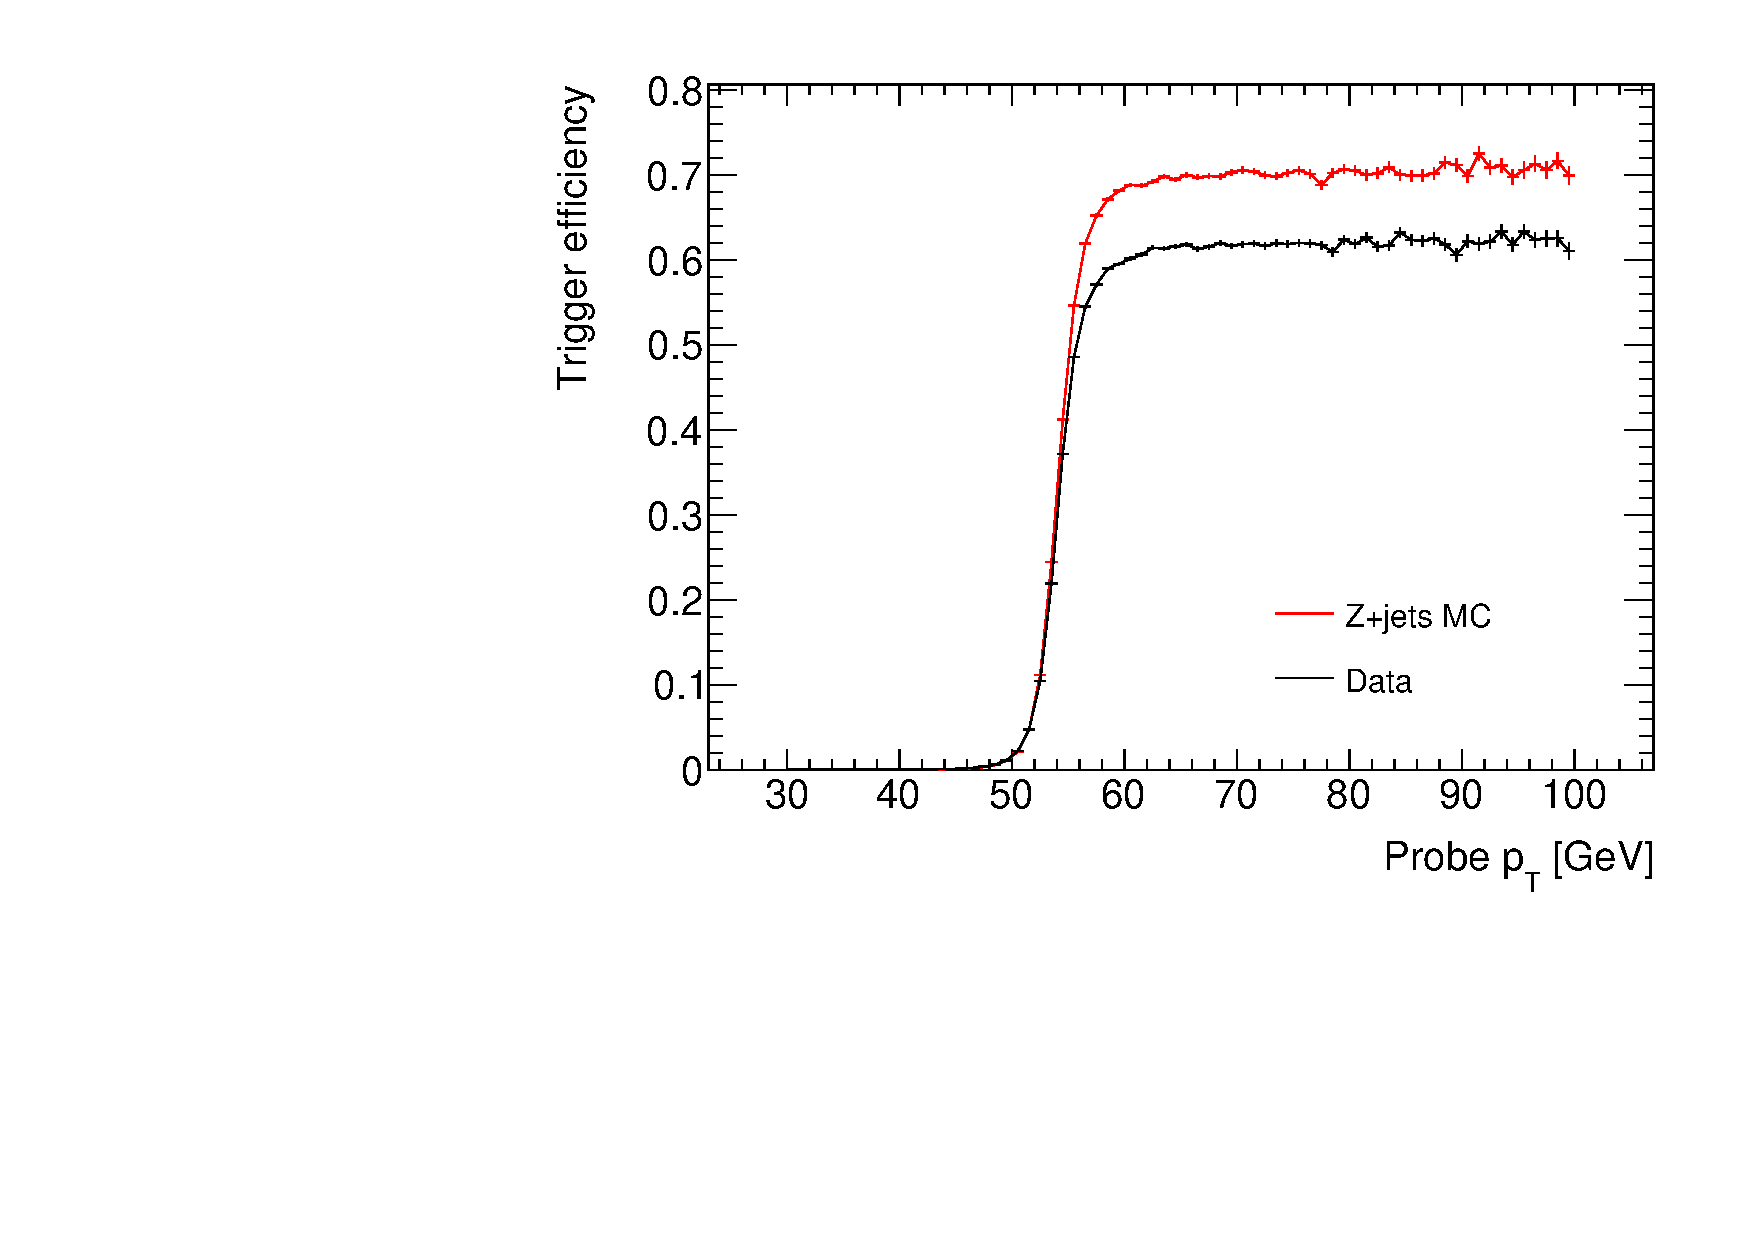
\includegraphics[width = 0.44 \textwidth]{figures/MuonTrigEff/simu_pt.pdf}}
    \subfloat[\label{fig:MuonTrigEff1Db}]{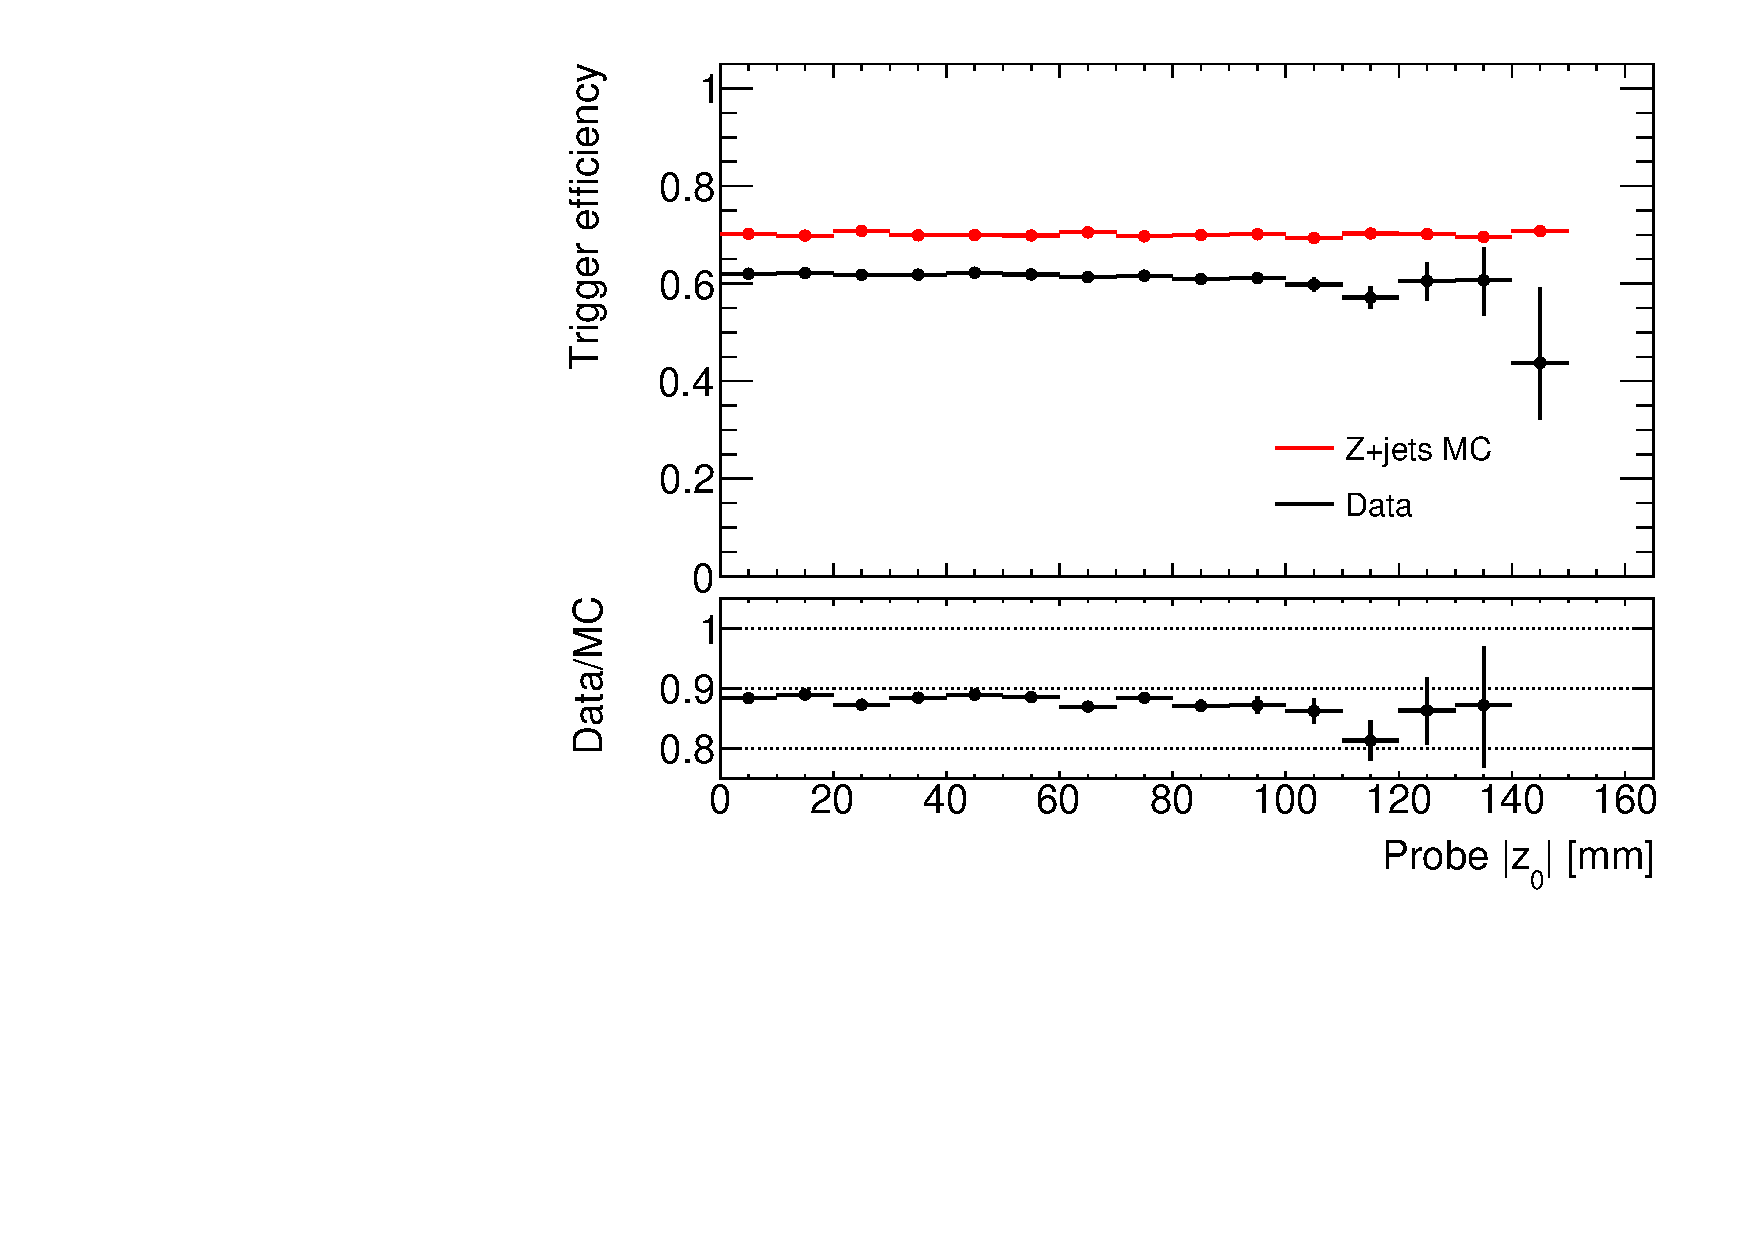
\includegraphics[width = 0.44 \textwidth]{figures/MuonTrigEff/simu_z0.pdf}}
    \caption{Efficiency of the single muon trigger as a function of the (a) $p_{T}$ and (b) |\zzero| of the probe in the data and $Z$+jets MC samples.
    }
    \label{fig:MuonTrigEff1D}
\end{figure}


\begin{figure}[!htb]
    \centering
    \subfloat[\label{fig:MuonTrigEff2Da}]{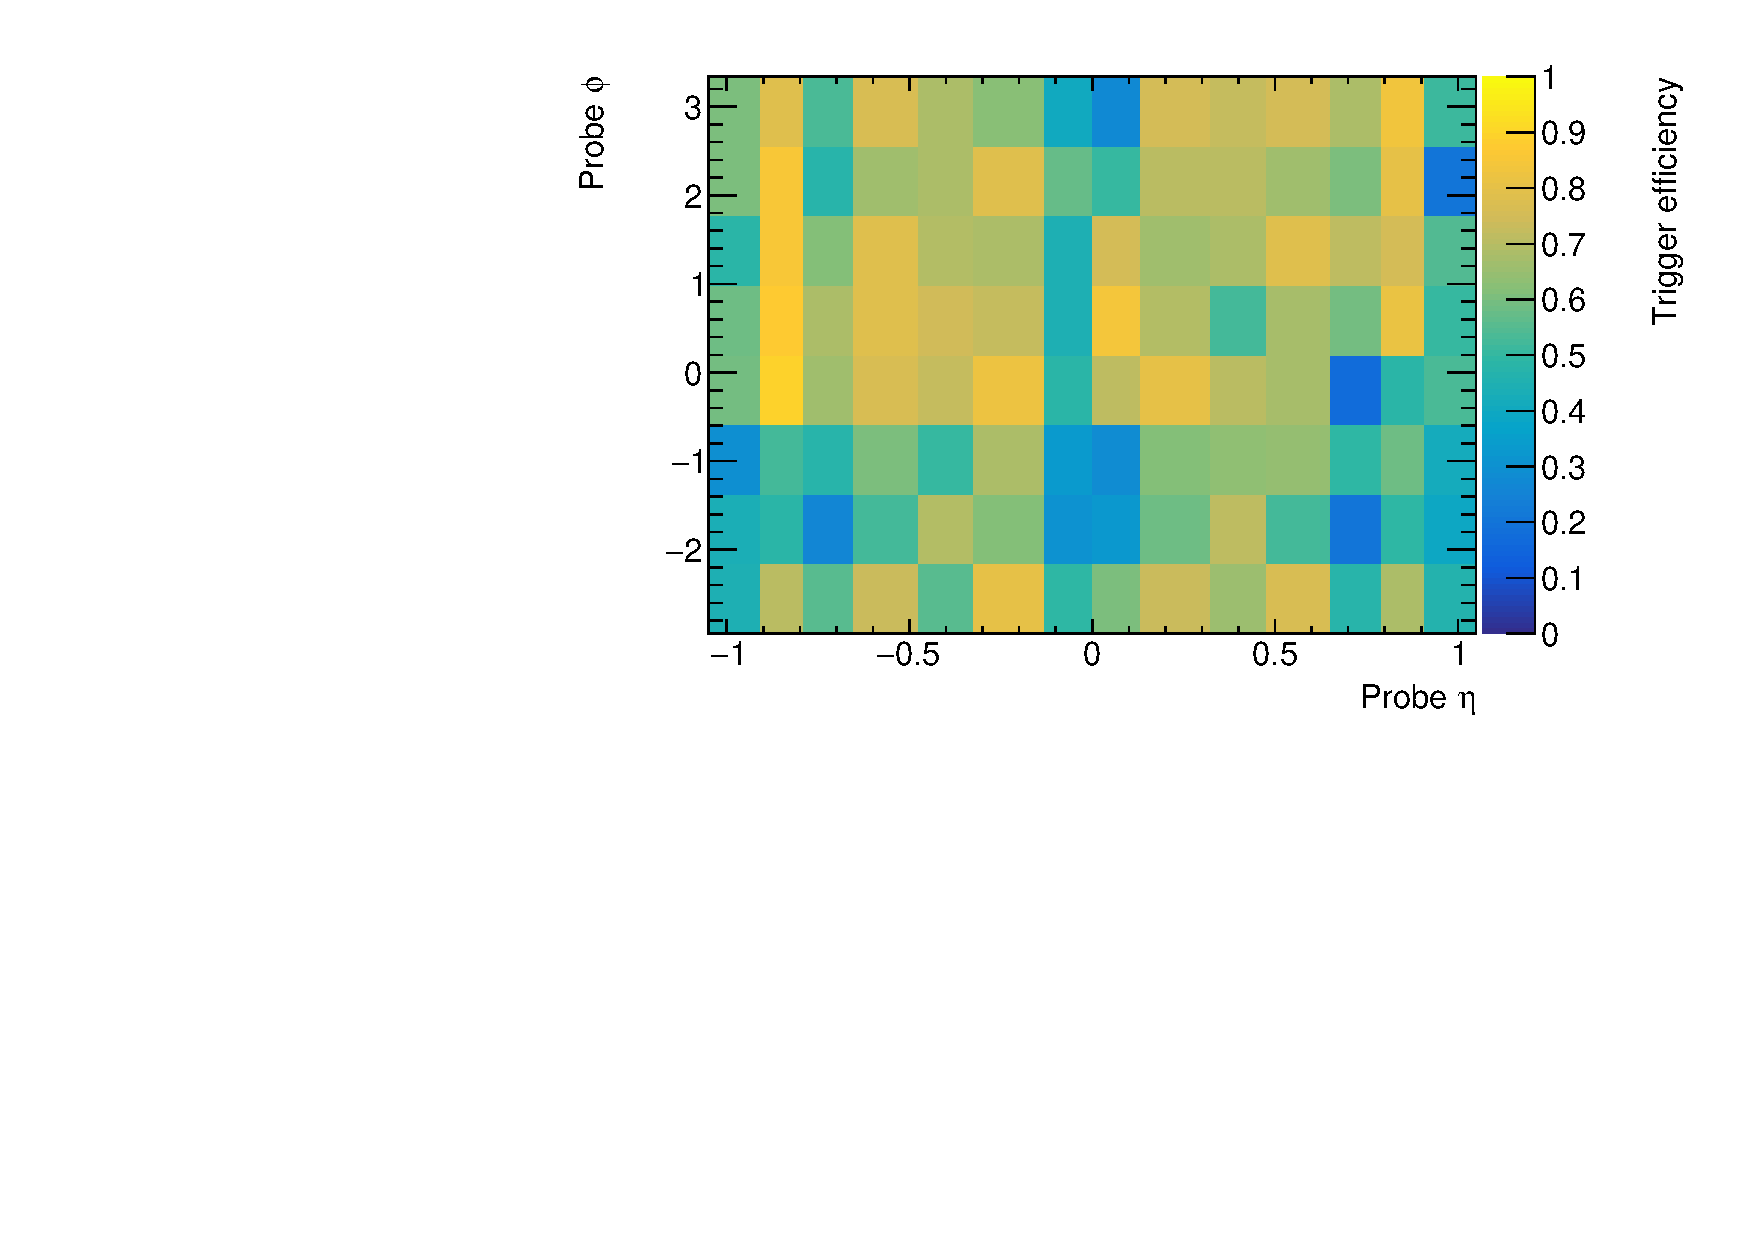
\includegraphics[width = 0.50 \textwidth]{figures/MuonTrigEff/simu_eta_phi_data.pdf}}
    \subfloat[\label{fig:MuonTrigEff2Db}]{\includegraphics[width = 0.50 \textwidth]{figures/MuonTrigEff/simu_eta_phi_MC.pdf}}
    \caption{Efficiency of the single muon trigger as a function the $\eta$ and $\phi$ of the probe in (a) data and (b) Z+jets MC sample.}
    \label{fig:MuonTrigEff2D}
\end{figure}

\subsection{Summary on Trigger Study}
The trigger studies show that the triggers have no dependence on the impact parameters up to $|d_{0}|\sim$120 and $|z_{0}|\sim$200 mm (Fig.~\ref{fig:signal_TrigEff}). Using the tag--and--probe method, scale factors are obtained, and the scale factors are summarized in Table~\ref{table:trigger_scale_factor}.

\begin{table}[!htb]
	\centering
	\begin{tabular}{cc}
		\hline
		\hline
		Trigger                                     & Scale factor \\
		\hline
        \texttt{HLT\_g140\_loose}                   & 0.988 \\
        \texttt{HLT\_g50\_loose}                    & 0.980 \\
        \texttt{HLT\_mu60\_0eta105\_msonly}         & 0.884 \\
		\hline
		\hline
	\end{tabular}
	\caption{Trigger scale factors from the tag--and--probe method.}
	\label{table:trigger_scale_factor}
\end{table}
These scale factors are binned in $\eta$ for the photon triggers and are binned in both $\eta$ and $\phi$ for the muon trigger to correct the signal efficiency. The overall trigger efficiency depends on the mass of $Z'$, 24-58\% for $\mu\mu$, 38-93\% for $ee$, and 17-88\% for $e\mu$ at $m > $ 250 GeV, and the trigger efficiency is much reduced for lower mass due to the $p_{T}$ threshold of the triggers.


\section{Lepton Reconstruction Efficiency}
\label{sec:tracking_efficiency}
The tracking efficiency, $\varepsilon_{\mathrm{track}}$, and the lepton identification efficiency, $\varepsilon_{\mathrm{lepton}}$, are studied together as a lepton reconstruction efficiency. The lepton reconstruction efficiency is defined and estimated as follows. From a signal MC sample, the leptons decaying from $Z'$ are collected at generator-level, referred as \textit{truth} signal leptons. For each truth signal lepton, if there is a reconstructed lepton with its ID track matched to the ID track of the truth signal lepton by a hit-based truth matching scheme, it is marked as reconstructed. The ratio of reconstructed signal leptons to the total number of signal leptons produced in the sample is taken as the lepton reconstruction efficiency. No \texttt{RPVLL} or trigger filter is applied in estimating the lepton reconstruction efficiency.

Figure~\ref{fig:lepton_eff} shows a representative plot of the lepton reconstruction efficiency as a function of track parameters using the combined signal MC samples of a $Z'$ decaying to all three channels, generated with $m = $ 250 GeV and $c\tau=$ 250 mm.

\begin{figure}[!htb]
    \centering
    \subfloat[]{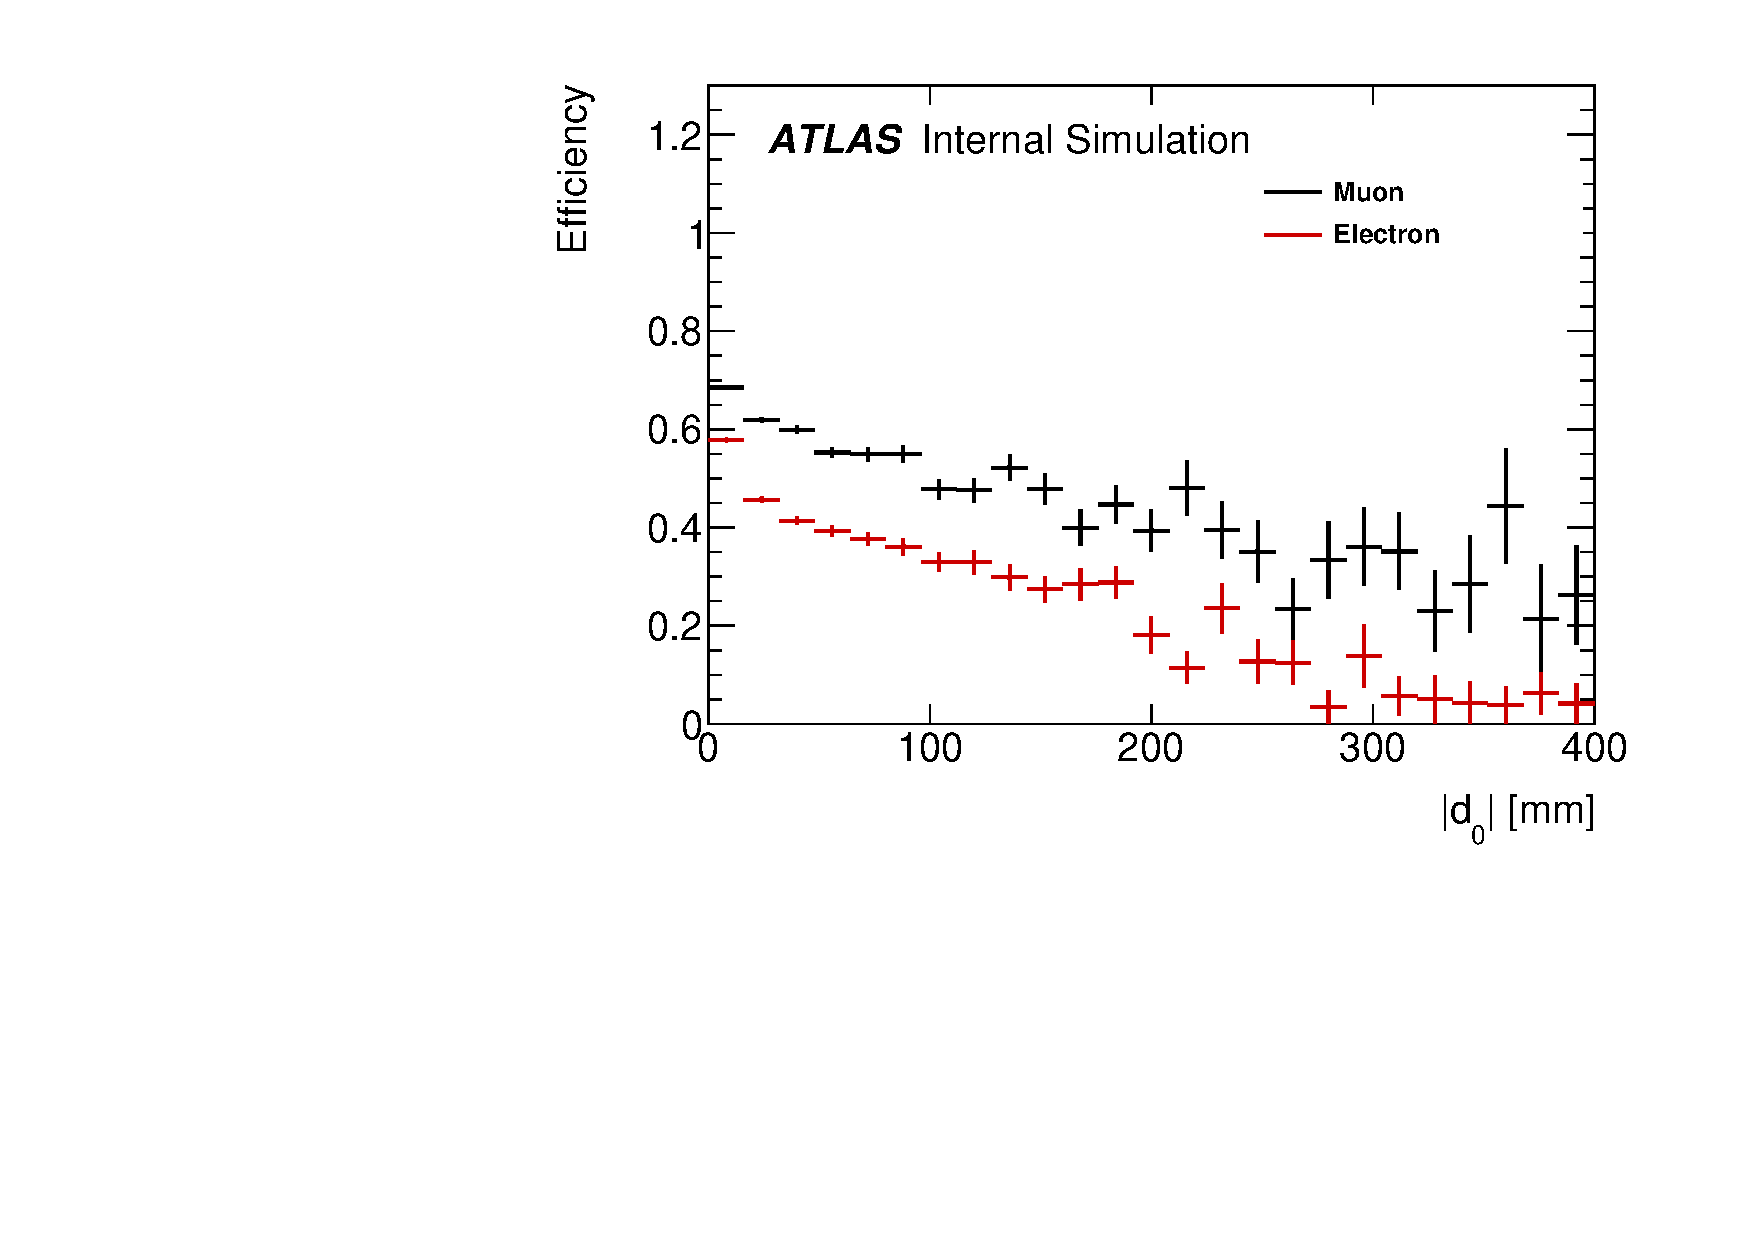
\includegraphics[width=0.50\textwidth]{figures/m_lepton_efficiency_d0.pdf}}
    \subfloat[]{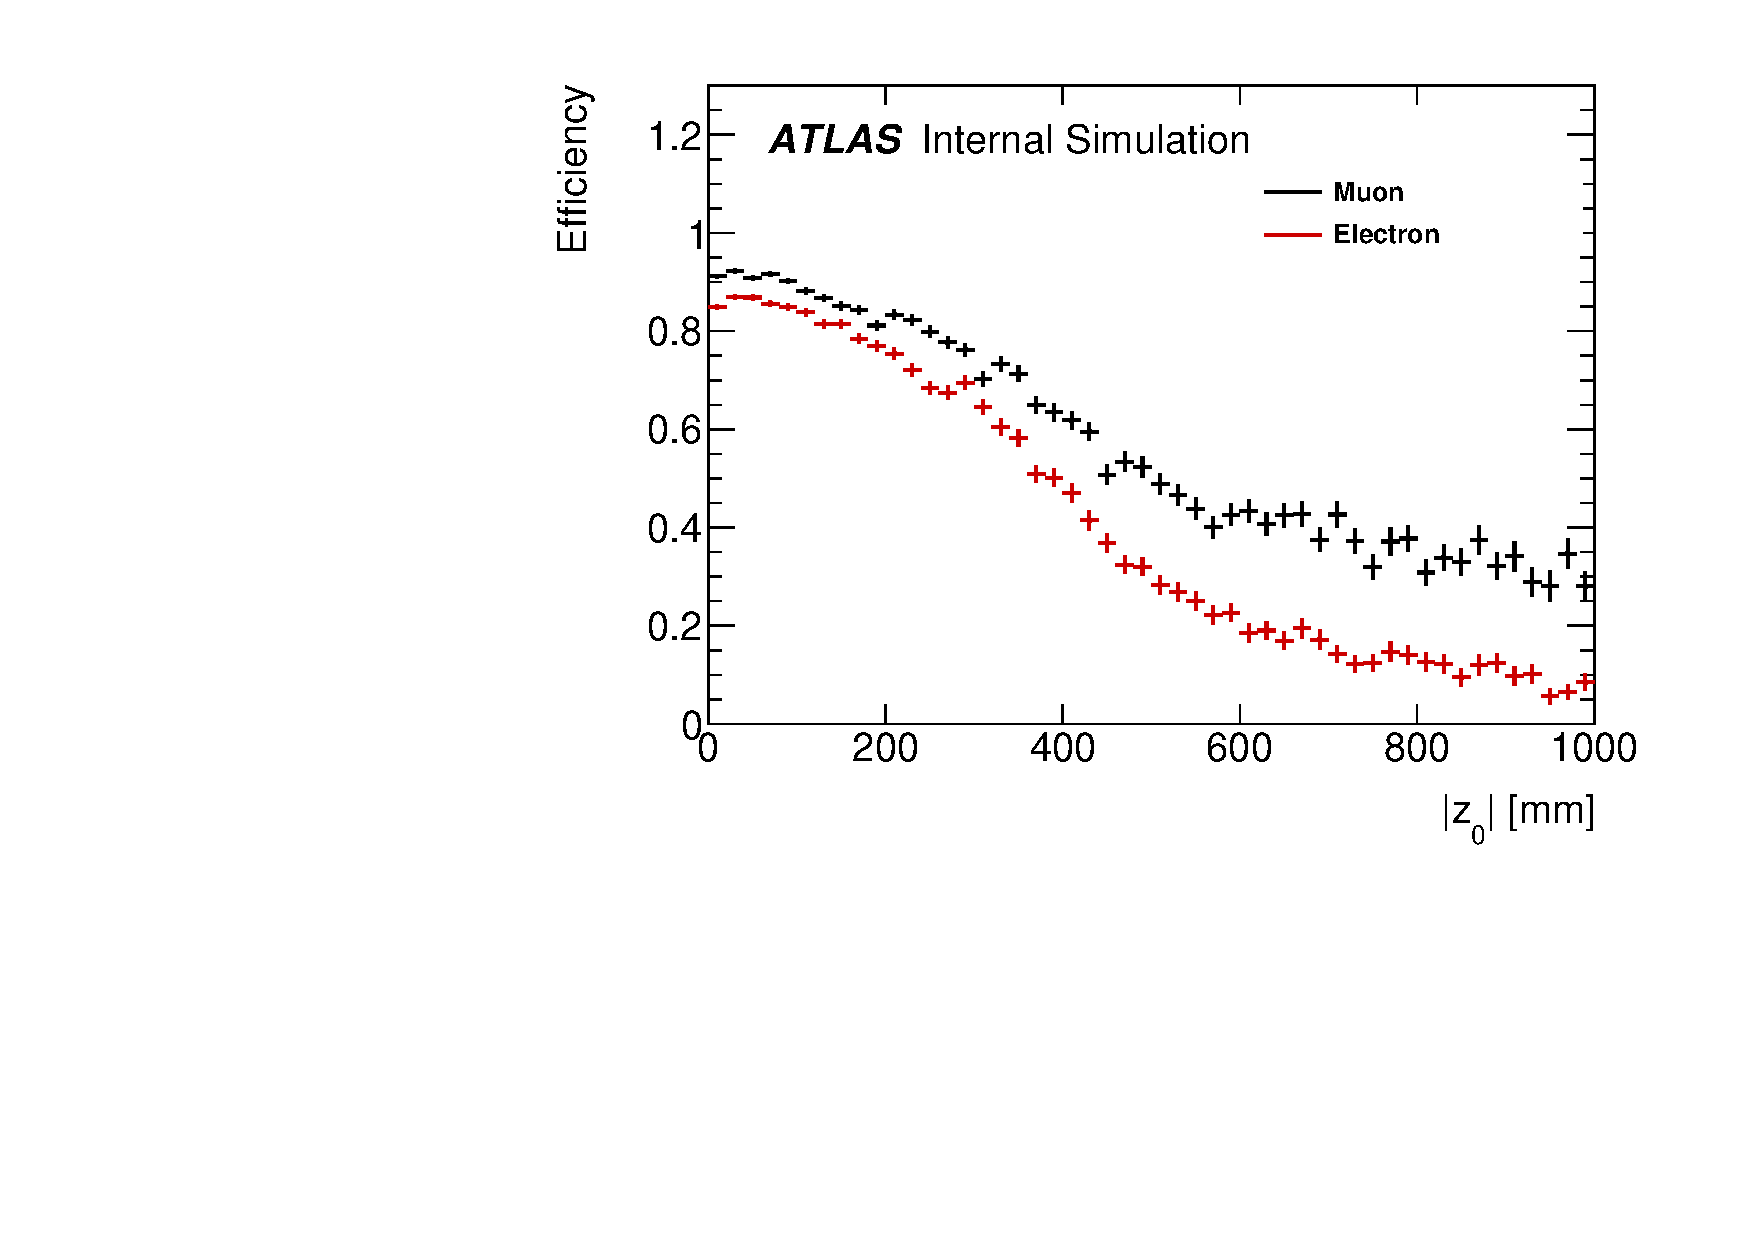
\includegraphics[width=0.50\textwidth]{figures/m_lepton_efficiency_z0.pdf}} \\
    \subfloat[]{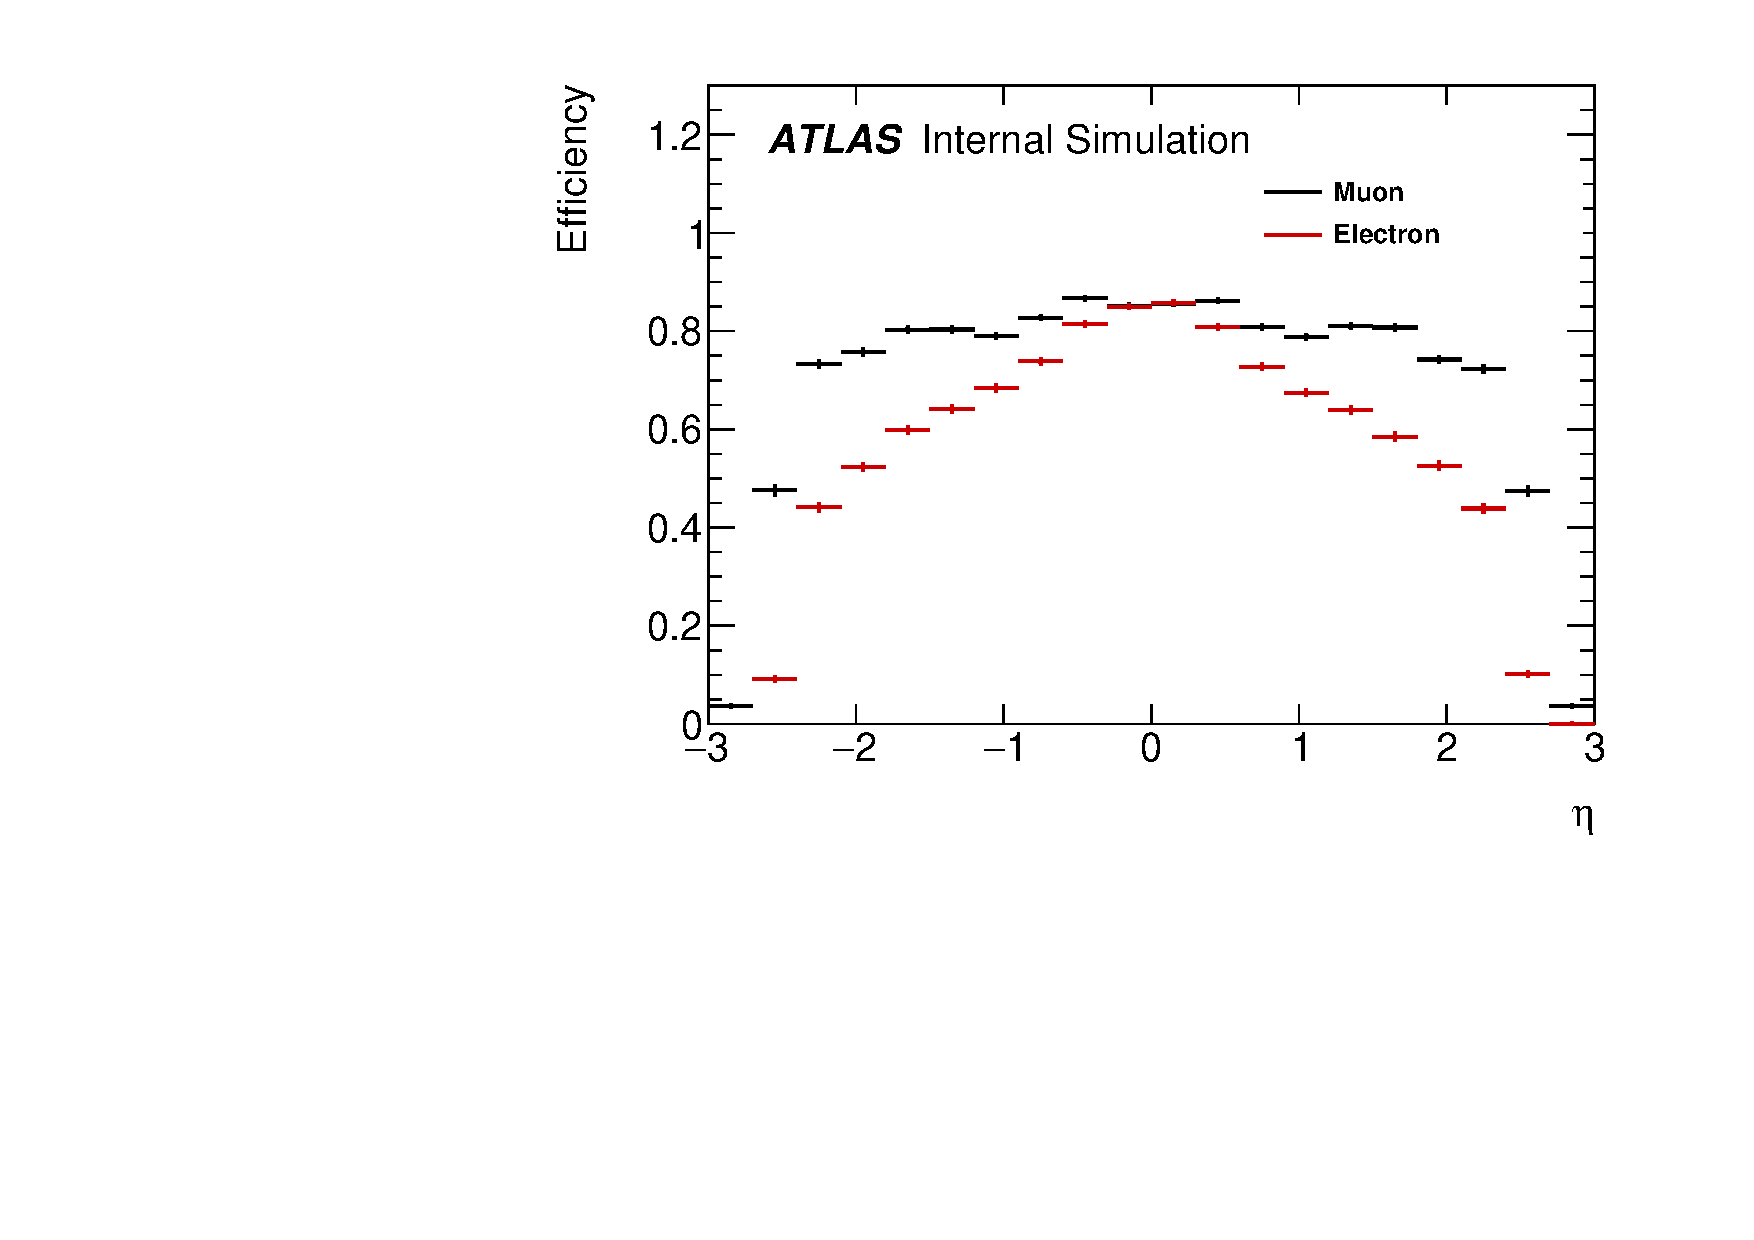
\includegraphics[width=0.50\textwidth]{figures/m_lepton_efficiency_eta.pdf}}
    \subfloat[]{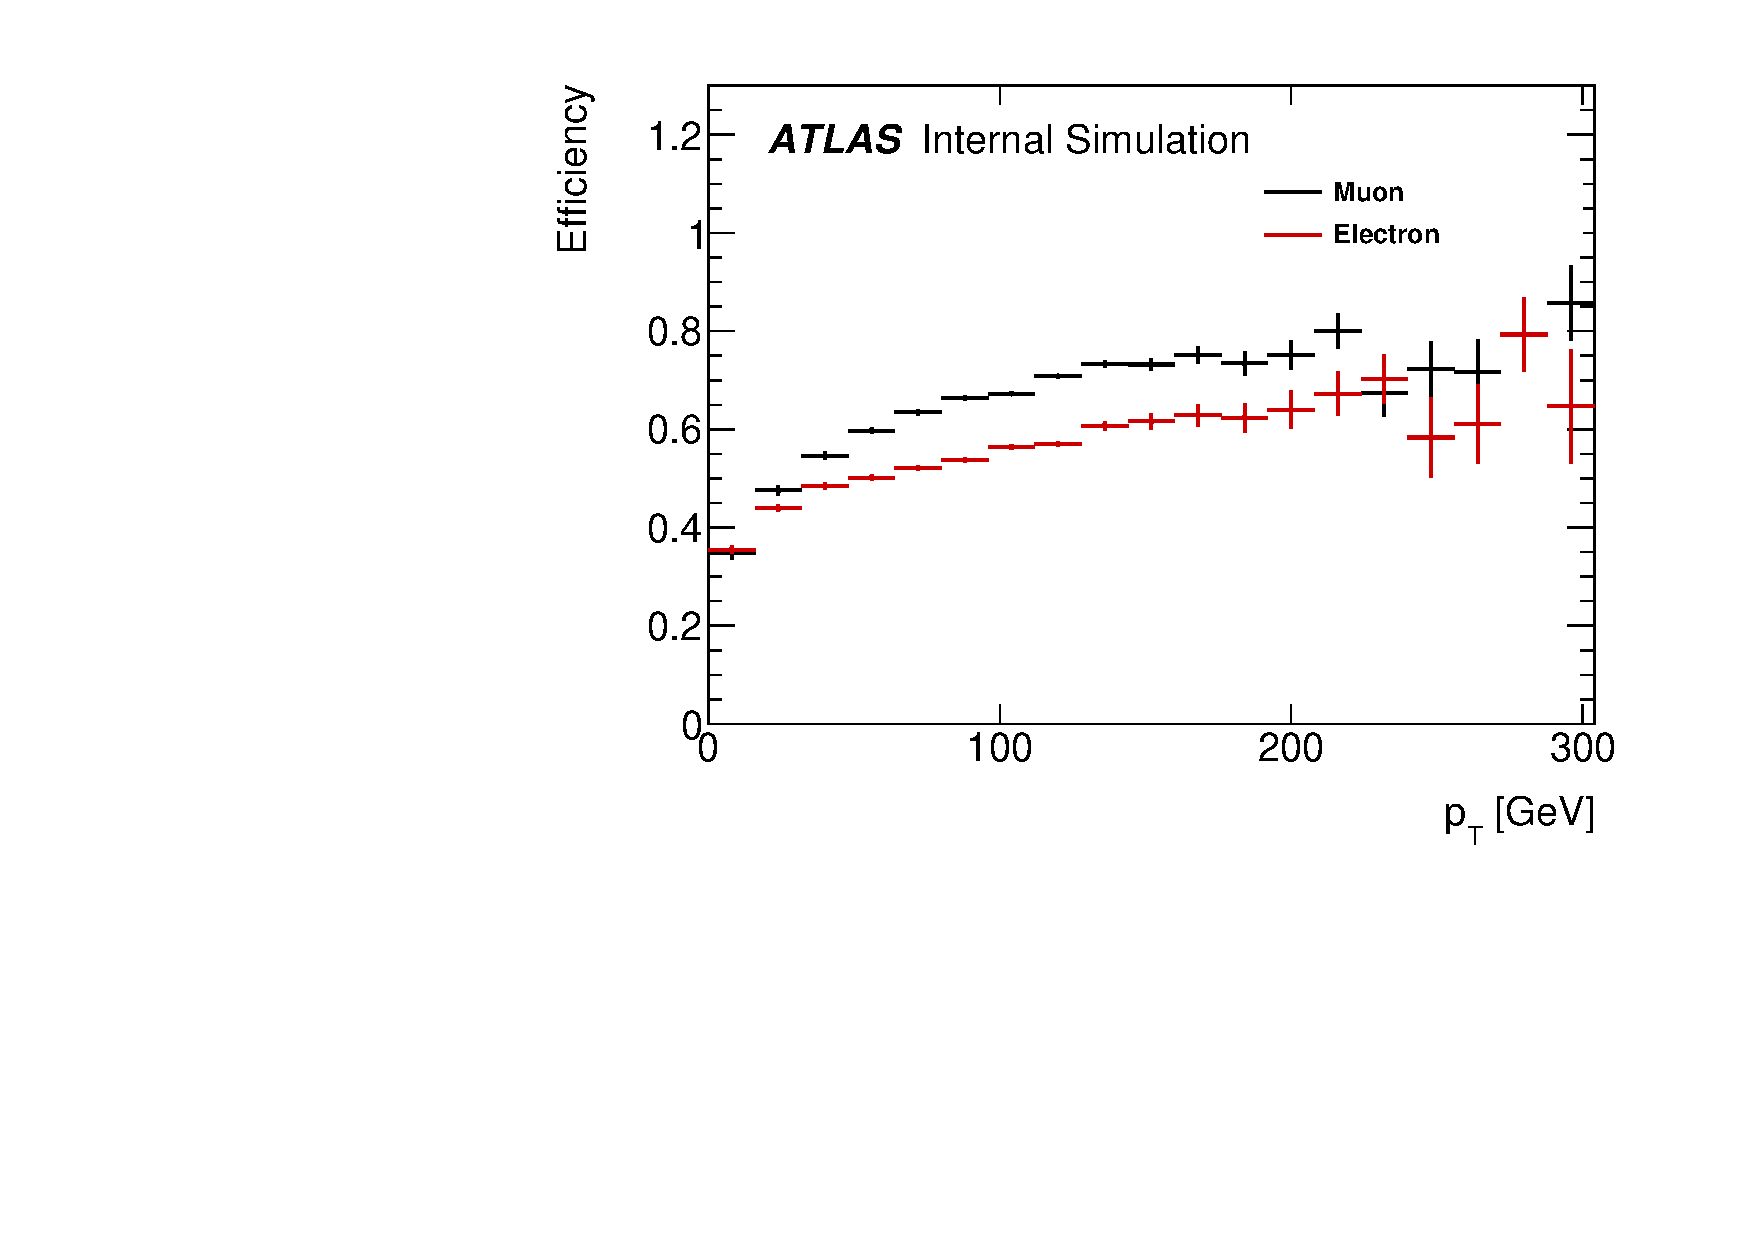
\includegraphics[width=0.50\textwidth]{figures/m_lepton_efficiency_pt.pdf}} 
    \caption{Lepton reconstruction efficiency as a function of (a) $d_{0}$, (b) $z_{0}$, (c) $\eta$, and (d) $p_{T}$ of signal leptons for the $Z'$ signal MC sample generated with $m=$ 250 GeV and $c\tau=$ 250 mm.}
    \label{fig:lepton_eff}
\end{figure}

It is evident that the efficiency decreases drastically at $|\eta| > 2.0$ where the Pixel barrel region ends due to the minimum silicon hits requirement on tracks as shown in Table~\ref{table:tracking}. The efficiency is not very sensitive to $p_{T}$ except in the low $p_{T}$ region ($p_{T} < 20$ GeV).

The lepton reconstruction efficiency decreases for large $d_{0}$ and $z_{0}$. In the signal MC samples, most of the $Z'$ decay within the Pixel barrel region, $r < $ 122.5 mm and $|z| < $ 400.5 mm, where the lepton reconstruction efficiency is high.

\section{Overall Reconstruction Efficiency}
\label{sec:combined_reco_efficiency}
The overall reconstruction efficiency represents the signal efficiency defined in Eq.~\ref{eq:OverallEff}, i.e. the ratio of $Z'$s reconstructed as displaced vertices in the signal region to the total $Z'$ produced in the sample. In this section, the signal selection cut flows (Section~\ref{sec:signal_cutflow}), the signal efficiency, and the efficiency distributions (Section~\ref{sec:efficiency}) are presented. In Section~\ref{sec:efficiency_map}, efficiency maps of the signal samples are presented as a function of $p_{T}$ and $|\eta|$ of $Z'$.

\subsection{Event and Vertex Cut Flow}
\label{sec:signal_cutflow}
The signal MC samples are processed as described in Section~\ref{sec:selection:pre}, in which long-lived $Z'$s are reconstructed as secondary vertices. The event and the vertex selections (Table~\ref{table:signal_selection}) are applied to the processed samples, and representative plots of the event vertex cut flow are shown in Fig.~\ref{fig:signal_cutflow_MC_mumu} using the signal MC samples of $Z'$ decaying to \mumu generated with $m=$ 250, 1000 GeV for $c\tau=$ 100 mm.

\begin{figure}[!htb]
    \centering
    \subfloat[]{\label{subfig:event_cutflow_MC}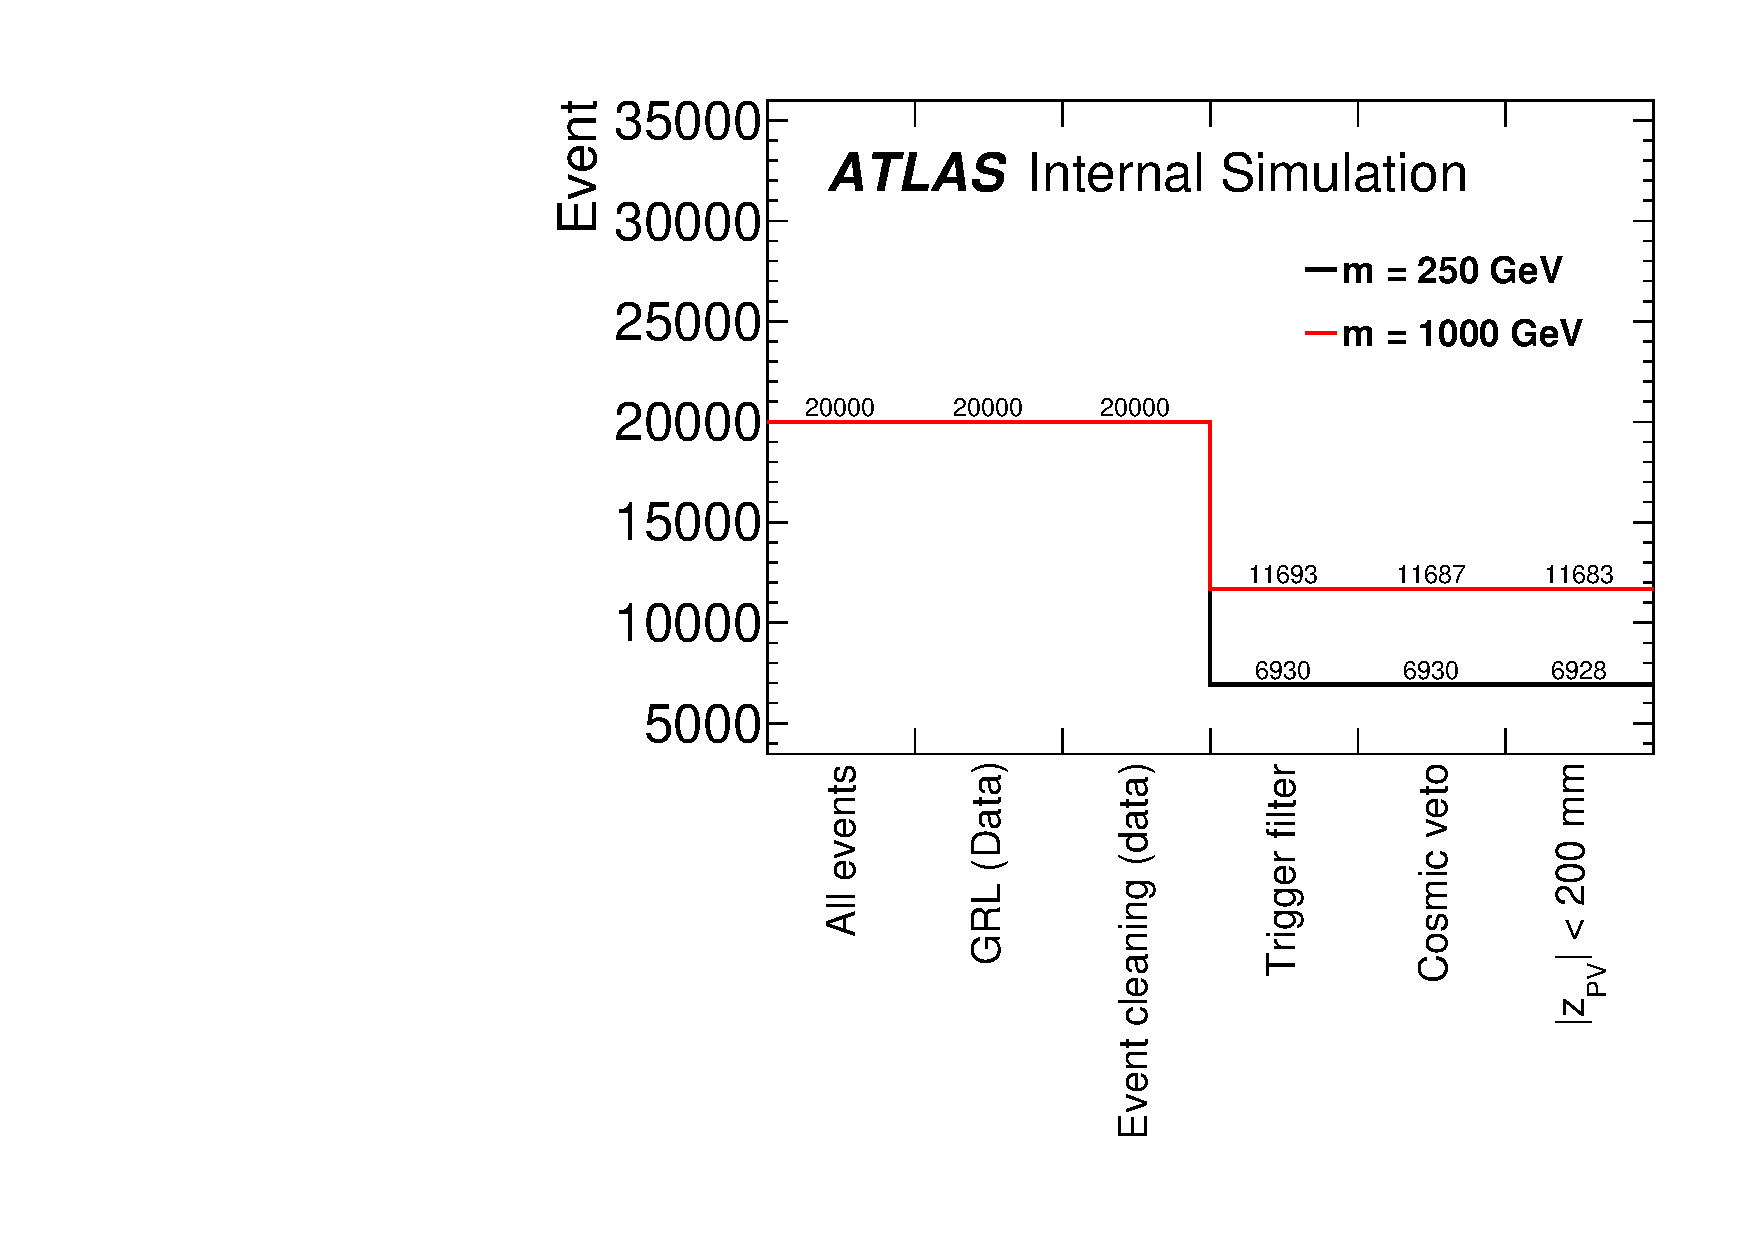
\includegraphics[width=0.5\textwidth]{figures/m_event_cutflow_MC_mumu.pdf}} 
    \subfloat[] {\label{subfig:vertex_cutflow_MC}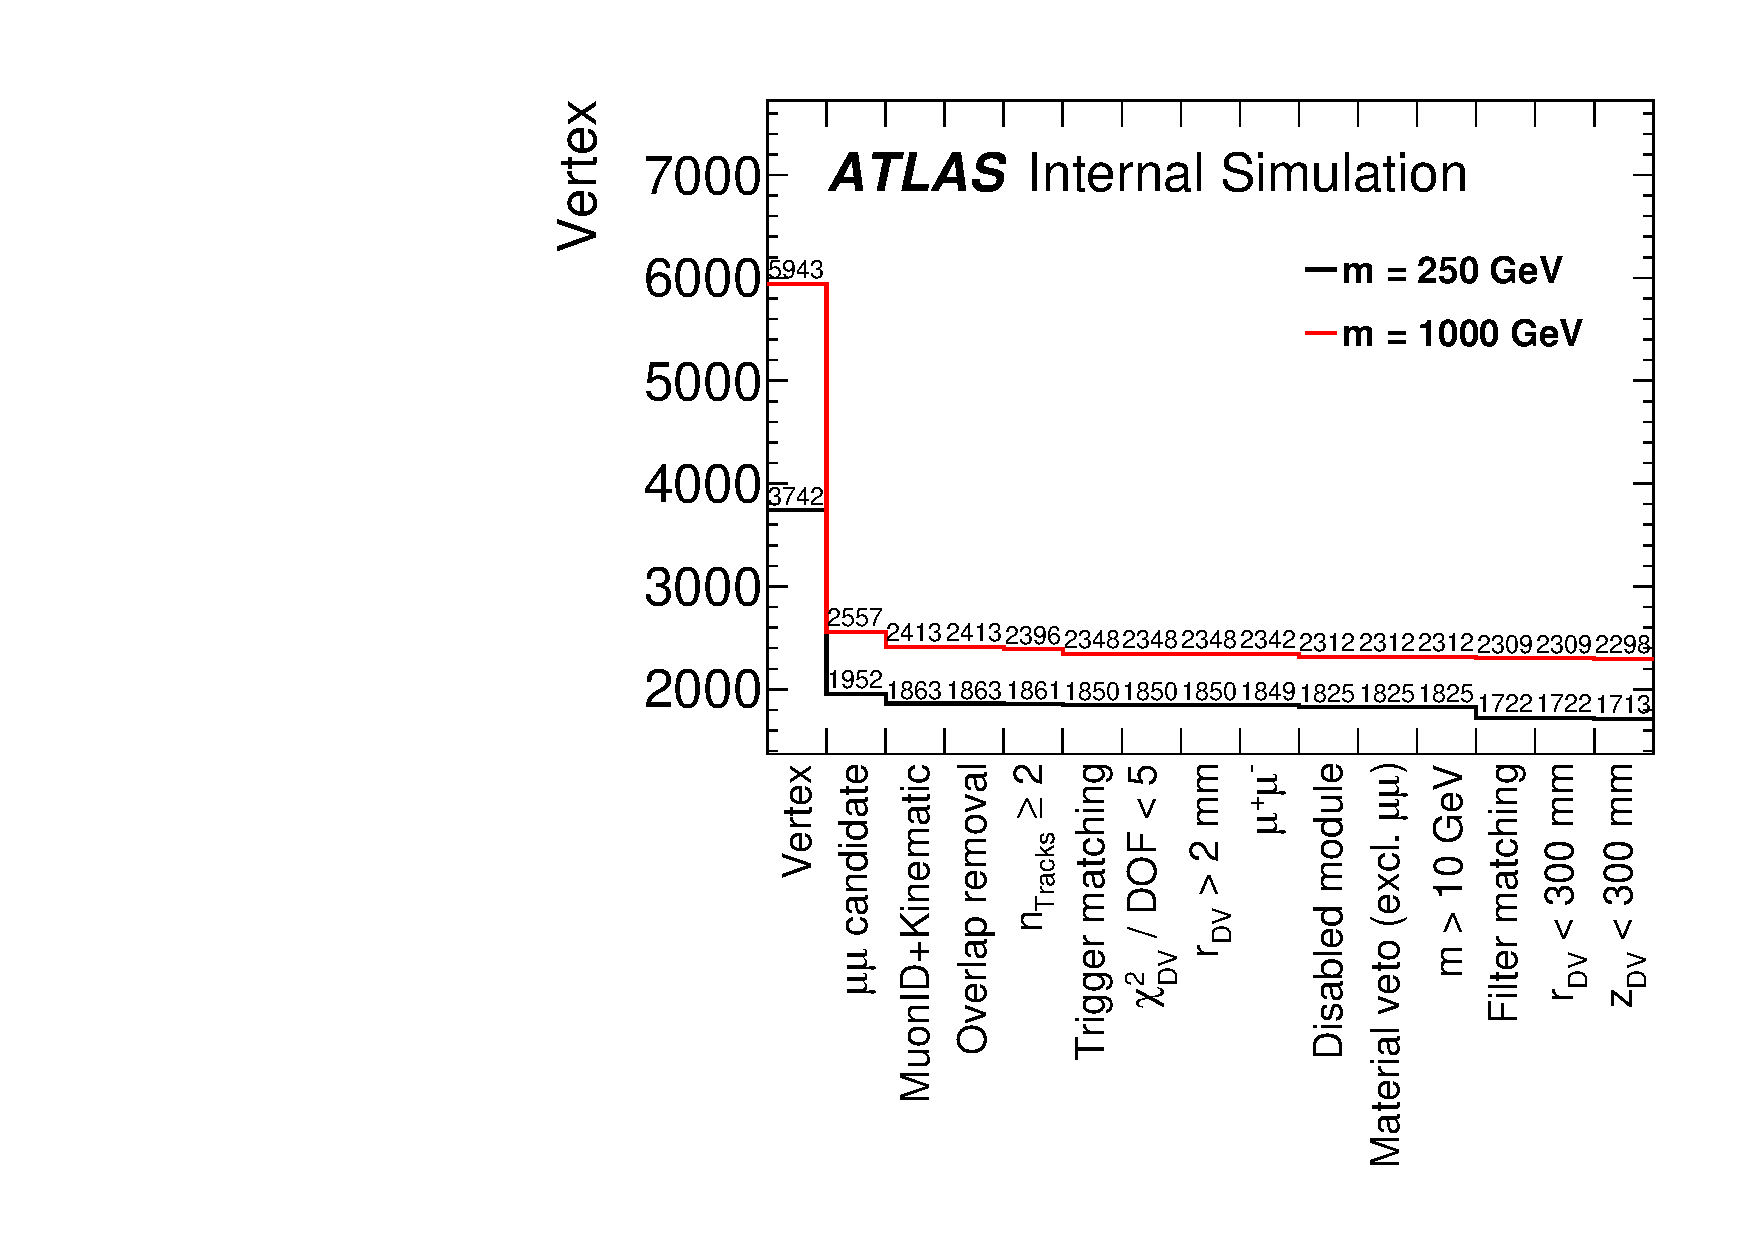
\includegraphics[width=0.5\textwidth]{figures/m_dv_cutflow_MC_mumu.pdf}} 
    \caption{(a) Event cut flow, and (b) vertex cut flow using the signal MC samples of $Z'\rightarrow \mumu$ generated with $m =$ 500, 1000 GeV for $c\tau= $ 100 mm.}
    \label{fig:signal_cutflow_MC_mumu}
\end{figure}

In the event cut flow, \texttt{GoodRunsList} filter and Event cleaning are shown as place holders as they are only applied to data sample. About 34-60$\%$ of the signal events passed the event cut flow, but the vertex cut flow shows that only about 18-25$\%$ of the signal events have a displaced vertex candidate, indicating that there is a significant loss of signal efficiency in the vertex reconstruction process. The following selection criteria, $\chi^{2} /$ DOF $<$ 5 and the displacement cut ($r_{\mathrm{DV}} > $ 2 mm), are applied, but the effect is very small as expected because the same requirements are applied in the secondary vertex reconstruction algorithm. A material veto is applied to all vertex types except \mumu vertex. The minimum dilepton mass requirement has minimum impact on the signal efficiency.

Events and vertex cut flow of other signal samples are shown in Tables~\ref{table:cutflow_all_mumu}$-$\ref{table:cutflow_all_emu}.


\begin{sidewaystable}[!htb]
  \centering
  %\subfloat[$Z'\rightarrow \mumu$]{
  \resizebox{\textwidth}{!}{
  \begin{tabular}{ c c c c c c c c c c c c c c c c c c c c c}
    \hline
    \hline
    $m_{Z'}$ (GeV) & $c\tau$ (mm)   & \rot{All events} 
                                    & \rot{Trigger filter} 
                                    & \rot{Cosmic veto} 
                                    & \rot{$|z_{PV}|<200$ mm} 
                                    & \rot{Vertex} 
                                    & \rot{$N_{\mu} \geq 2$ }
                                    & \rot{Muon selection} 
                                    & \rot{Overlap removal}
                                    & \rot{$N_{\mu}=2$}
                                    & \rot{Trigger matching}
                                    & \rot{$\chi^{2} /$ DOF $< 5$}
                                    & \rot{$r_{\mathrm{DV}} >$ 2 mm}
                                    & \rot{\mumu}
                                    & \rot{Disabled module}
                                    & \rot{$m > 10$ GeV}
                                    & \rot{Filter matching}
                                    & \rot{$r_{\mathrm{DV}} < 300$ mm}
                                    & \rot{$|z_{DV}| < 300$ mm} \\
    \hline
    100&	100&	20000&	940&	940&	940&	644&	366&	342&	342&	339&	339&	339&	339&	339&	330&	330&	108&	108&	106 \\
    100&	250&	20000&	818&	818&	818&	533&	269&	260&	260&	260&	259&	259&	259&	259&	252&	252&	82&	82&	81 \\
    100&	500&	20000&	761&	761&	761&	416&	165&	154&	154&	154&	154&	154&	154&	154&	148&	148&	50&	50&	49 \\
    250&	100&	20000&	6930&	6930&	6928&	3742&	1952&	1863&	1863&	1861&	1850&	1850&	1850&	1849&	1825&	1825&	1722&	1722&	1713 \\
    250&	250&	20000&	6180&	6179&	6176&	3467&	1809&	1708&	1708&	1703&	1700&	1700&	1700&	1699&	1677&	1677&	1605&	1605&	1582 \\
    250&	500&	20000&	4922&	4921&	4921&	2680&	1354&	1284&	1284&	1278&	1276&	1276&	1276&	1276&	1261&	1261&	1205&	1205&	1176 \\
    500&	100&	19000&	9146&	9145&	9144&	4680&	2205&	2091&	2091&	2085&	2068&	2068&	2068&	2068&	2047&	2047&	2042&	2042&	2034 \\
    500&	250&	20000&	8273&	8272&	8269&	4481&	2191&	2080&	2080&	2068&	2056&	2056&	2056&	2054&	2024&	2024&	2023&	2023&	2007 \\
    500&	500&	20000&	6724&	6720&	6717&	3605&	1777&	1666&	1666&	1658&	1646&	1646&	1646&	1646&	1617&	1617&	1611&	1611&	1572 \\
    750&	100&	20000&	11032&	11028&	11027&	5605&	2473&	2330&	2330&	2313&	2282&	2282&	2282&	2281&	2267&	2267&	2254&	2254&	2250 \\
    750&	250&	20000&	9622&	9616&	9613&	5301&	2626&	2457&	2457&	2441&	2421&	2421&	2421&	2419&	2391&	2391&	2386&	2385&	2364 \\
    750&	500&	20000&	8059&	8055&	8054&	4262&	2017&	1878&	1878&	1868&	1851&	1851&	1851&	1849&	1824&	1824&	1820&	1819&	1784 \\
    1000&	100&	20000&	11693&	11687&	11683&	5943&	2557&	2413&	2413&	2396&	2348&	2348&	2348&	2342&	2312&	2312&	2309&	2309&	2298 \\
    1000&	250&	20000&	10517&	10515&	10514&	5804&	2725&	2578&	2578&	2564&	2518&	2518&	2517&	2512&	2479&	2479&	2476&	2476&	2457 \\
    1000&	500&	20000&	8905&	8902&	8901&	4878&	2295&	2170&	2170&	2155&	2129&	2129&	2129&	2117&	2092&	2092&	2089&	2089&	2058 \\
    \hline
    \hline
  \end{tabular}
  }
  %}
  \caption{Event and vertex cut flow of the signal MC sample of $Z' \rightarrow \mumu$.}
  \label{table:cutflow_all_mumu}
\end{sidewaystable}

%\begin{sidewaystable}[!htb]\ContinuedFloat
\begin{sidewaystable}[!htb]
  \centering
  %\subfloat[$Z'\rightarrow \ee$]{
  \resizebox{\textwidth}{!}{
  \begin{tabular}{ c c c c c c c c c c c c c c c c c c c c c c}
    \hline
    \hline
    $m_{Z'}$ (GeV) & $c\tau$ (mm)   & \rot{All events} 
                                    & \rot{Trigger filter} 
                                    & \rot{Cosmic veto} 
                                    & \rot{$|z_{PV}|<200$ mm} 
                                    & \rot{Vertex} 
                                    & \rot{$N_{e} \geq 2$ }
                                    & \rot{Electron selection} 
                                    & \rot{Bad cluster} 
                                    & \rot{Overlap removal}
                                    & \rot{$N_{e} = 2$}
                                    & \rot{Trigger matching}
                                    & \rot{$\chi^{2} /$ DOF $< 5$}
                                    & \rot{$r_{\mathrm{DV}} > 2$ mm}
                                    & \rot{\ee}
                                    & \rot{Disabled module}
                                    & \rot{Material veto}
                                    & \rot{$m > 10$ GeV}
                                    & \rot{Filter matching}
                                    & \rot{$r_{\mathrm{DV}} < 300$ mm}
                                    & \rot{$|z_{DV}| < 300$ mm} \\
    \hline
    100&	100&	20000&	315&	315&	315&	166&	71&	69&	69&	67&	67&	66&	66&	66&	66&	65&	52&	52&	16&	16&	15 \\
    100&	250&	20000&	323&	323&	323&	145&	61&	59&	58&	56&	56&	56&	56&	56&	56&	55&	36&	36&	15&	15&	15 \\
    100&	500&	20000&	241&	241&	241&	111&	31&	30&	29&	29&	29&	27&	27&	27&	27&	26&	19&	19&	10&	10&	9 \\
    250&	100&	20000&	10147&	10145&	10144&	4472&	1696&	1658&	1639&	1618&	1601&	1585&	1585&	1585&	1577&	1563&	1378&	1378&	1345&	1345&	1339 \\
    250&	250&	20000&	9276&	9274&	9272&	4083&	1576&	1519&	1501&	1477&	1458&	1453&	1453&	1453&	1448&	1417&	1206&	1206&	1174&	1174&	1163 \\
    250&	500&	20000&	7755&	7750&	7749&	3203&	1105&	1063&	1057&	1038&	1017&	1011&	1011&	1011&	1007&	987&	803&	803&	769&	769&	758 \\
    500&	100&	20000&	16012&	16008&	16006&	6621&	2017&	1940&	1925&	1900&	1878&	1877&	1877&	1877&	1857&	1843&	1668&	1668&	1656&	1656&	1652 \\
    500&	250&	20000&	14855&	14853&	14849&	6245&	1986&	1907&	1892&	1880&	1858&	1858&	1858&	1857&	1844&	1824&	1580&	1580&	1569&	1569&	1559 \\
    500&	500&	19000&	12279&	12278&	12276&	5029&	1566&	1505&	1502&	1493&	1471&	1466&	1466&	1466&	1455&	1432&	1194&	1194&	1185&	1185&	1162 \\
    750&	100&	20000&	18014&	18011&	18006&	7422&	2266&	2196&	2182&	2173&	2138&	2138&	2138&	2138&	2092&	2085&	1919&	1919&	1914&	1914&	1913 \\
    750&	250&	20000&	16920&	16914&	16912&	7165&	2260&	2186&	2177&	2168&	2129&	2129&	2129&	2129&	2099&	2081&	1832&	1832&	1824&	1824&	1808 \\
    750&	500&	20000&	15290&	15286&	15283&	6206&	1853&	1791&	1778&	1768&	1731&	1731&	1731&	1731&	1711&	1690&	1423&	1423&	1419&	1419&	1399 \\
    1000&	100&	20000&	18723&	18719&	18714&	7749&	2347&	2271&	2247&	2235&	2195&	2195&	2195&	2195&	2162&	2151&	2004&	2004&	1996&	1996&	1992 \\
    1000&	250&	20000&	17890&	17883&	17877&	7674&	2487&	2412&	2401&	2395&	2349&	2349&	2349&	2349&	2320&	2298&	2070&	2070&	2067&	2067&	2050 \\
    1000&	500&	19000&	15666&	15660&	15658&	6507&	1956&	1881&	1870&	1866&	1842&	1842&	1842&	1842&	1812&	1797&	1562&	1562&	1559&	1559&	1548 \\
    \hline
    \hline
  \end{tabular}
  }
  %}
  \caption{Event and vertex cut flow of the signal MC sample of $Z' \rightarrow \ee$.}
  \label{table:cutflow_all_ee}
\end{sidewaystable}

%\begin{sidewaystable}[!htb]\ContinuedFloat
\begin{sidewaystable}[!htb]
  \centering
  %\subfloat[$Z'\rightarrow \emu$]{
  \resizebox{\textwidth}{!}{
  \begin{tabular}{ c c c c c c c c c c c c c c c c c c c c c c}
    \hline
    \hline
    $m_{Z'}$ (GeV) & $c\tau$ (mm)   & \rot{All events} 
                                    & \rot{Trigger filter} 
                                    & \rot{Cosmic veto} 
                                    & \rot{$|z_{PV}| < 200$ mm} 
                                    & \rot{Vertex} 
                                    & \rot{$N_{\ell} \geq 2$ }
                                    & \rot{Electron selection} 
                                    & \rot{Bad cluster} 
                                    & \rot{Overlap removal}
                                    & \rot{$N_{\ell} = 2$}
                                    & \rot{Trigger matching}
                                    & \rot{$\chi^{2} /$ DOF $< 5$}
                                    & \rot{$r_{\mathrm{DV}} > 2$ mm}
                                    & \rot{\emu}
                                    & \rot{Disabled module}
                                    & \rot{Material veto}
                                    & \rot{$m > 10$ GeV}
                                    & \rot{Filter matching}
                                    & \rot{$r_{\mathrm{DV}} < 300$ mm}
                                    & \rot{$|z_{DV}| < 300$ mm} \\
    \hline
    100&	100&	19000&	484&	484&	484&	295&	150&	145&	145&	137&	136&	134&	134&	134&	134&	127&	88&	88&	26&	26&	26 \\
    100&	250&	20000&	483&	483&	483&	255&	94&	91&	91&	89&	88&	88&	88&	88&	88&	87&	61&	61&	21&	21&	19 \\
    100&	500&	19000&	379&	379&	379&	178&	56&	53&	53&	53&	53&	53&	53&	53&	53&	50&	34&	34&	15&	15&	14 \\
    250&	100&	20000&	4771&	4769&	4768&	2326&	960&	938&	934&	899&	891&	868&	868&	868&	862&	851&	729&	729&	698&	698&	696 \\
    250&	250&	20000&	4273&	4272&	4265&	2251&	921&	901&	899&	874&	867&	848&	848&	848&	844&	829&	682&	682&	650&	650&	638 \\
    250&	500&	20000&	3486&	3484&	3481&	1667&	709&	695&	693&	678&	672&	663&	663&	663&	662&	653&	532&	532&	511&	511&	502 \\
    500&	100&	19000&	13351&	13349&	13346&	6049&	2168&	2135&	2131&	2040&	2019&	2005&	2005&	2005&	1999&	1981&	1793&	1793&	1736&	1736&	1728 \\
    500&	250&	20000&	12680&	12680&	12679&	5736&	2199&	2169&	2160&	2059&	2037&	2020&	2020&	2019&	2016&	1990&	1748&	1748&	1688&	1688&	1671 \\
    500&	500&	20000&	10885&	10883&	10883&	4797&	1732&	1697&	1689&	1623&	1604&	1595&	1594&	1594&	1581&	1552&	1327&	1327&	1264&	1264&	1239 \\
    750&	100&	19000&	16046&	16036&	16032&	7041&	2624&	2590&	2582&	2480&	2448&	2437&	2437&	2436&	2408&	2400&	2232&	2232&	2207&	2207&	2203 \\
    750&	250&	20000&	15546&	15545&	15541&	7171&	2706&	2659&	2655&	2533&	2502&	2494&	2493&	2492&	2475&	2448&	2172&	2172&	2142&	2142&	2115 \\
    750&	500&	20000&	13598&	13590&	13585&	6033&	2170&	2132&	2125&	2025&	2003&	1995&	1995&	1995&	1983&	1965&	1686&	1686&	1644&	1644&	1604 \\
    1000&	100&	18000&	15970&	15963&	15959&	7189&	2581&	2543&	2535&	2415&	2385&	2371&	2371&	2370&	2345&	2323&	2163&	2163&	2148&	2148&	2146 \\
    1000&	250&	20000&	16751&	16743&	16739&	7835&	3088&	3036&	3028&	2899&	2856&	2854&	2854&	2854&	2832&	2809&	2512&	2512&	2495&	2495&	2475 \\
    1000&	500&	19000&	14165&	14160&	14154&	6366&	2345&	2290&	2284&	2198&	2162&	2153&	2153&	2152&	2134&	2112&	1826&	1825&	1808&	1808&	1773 \\
    \hline
    \hline
  \end{tabular}
  }
  %}
  \caption{Event and vertex cut flow of the signal MC sample of $Z' \rightarrow \emu$.}
  \label{table:cutflow_all_emu}
\end{sidewaystable}




\subsection{Signal Efficiency and Distribution}
\label{sec:efficiency}

The signal efficiency is studied by examining the efficiency distributions in the transverse ($r$), longitudinal ($z$) vertex position, and the $\eta$ and $\phi$ distributions of the signal vertices. The representative efficiency distributions are shown in Figure~\ref{fig:signal_vertex_dist} using the signal MC samples generated with $m =$ 500, 1000 GeV for $c\tau=$ 100 mm.

\begin{figure}[!htb]
    \centering
    \subfloat[]{\label{subfig:vertex_dist_r}\includegraphics[width=0.49\textwidth]{figures/m_eff_dv_r.pdf}}
    \subfloat[]{\label{subfig:vertex_dist_z}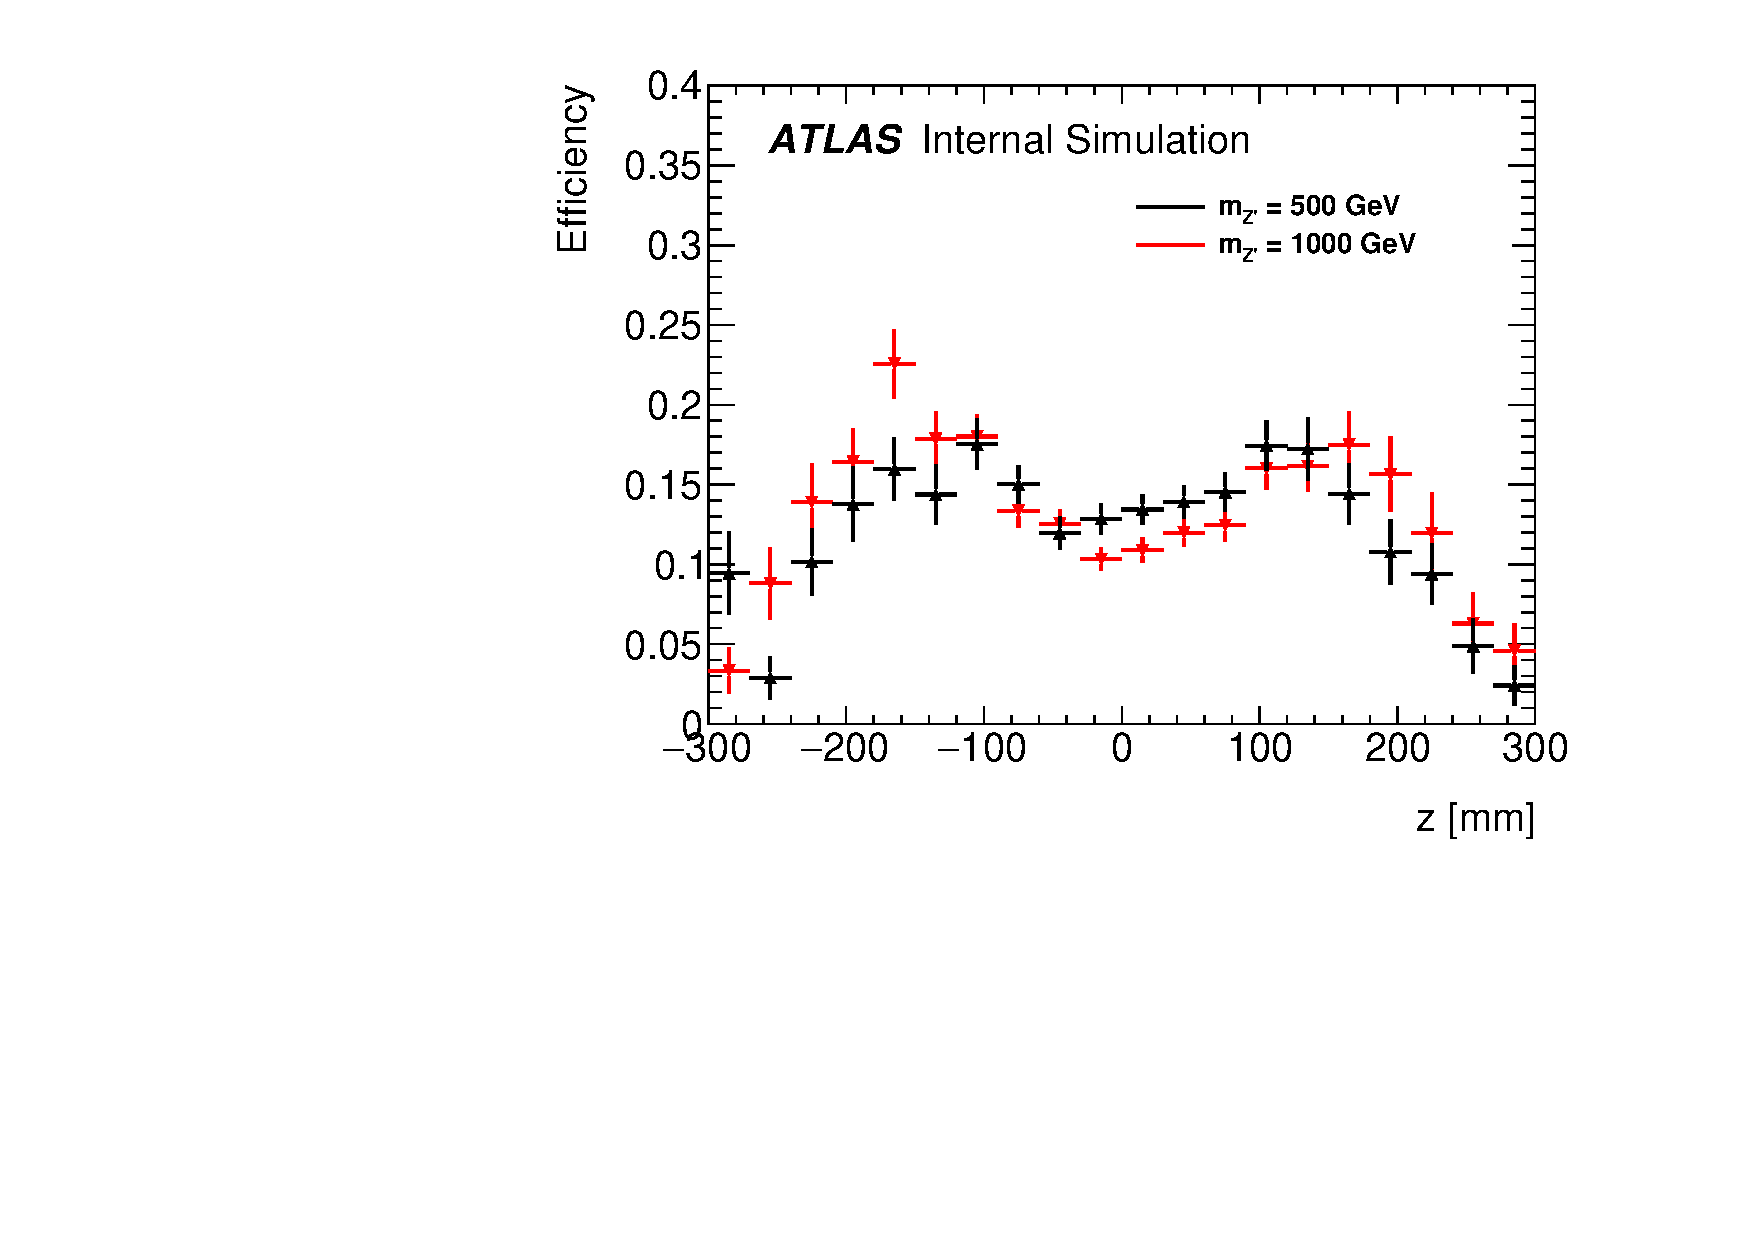
\includegraphics[width=0.49\textwidth]{figures/m_eff_dv_z.pdf}} \\
    \subfloat[]{\label{subfig:vertex_dist_eta}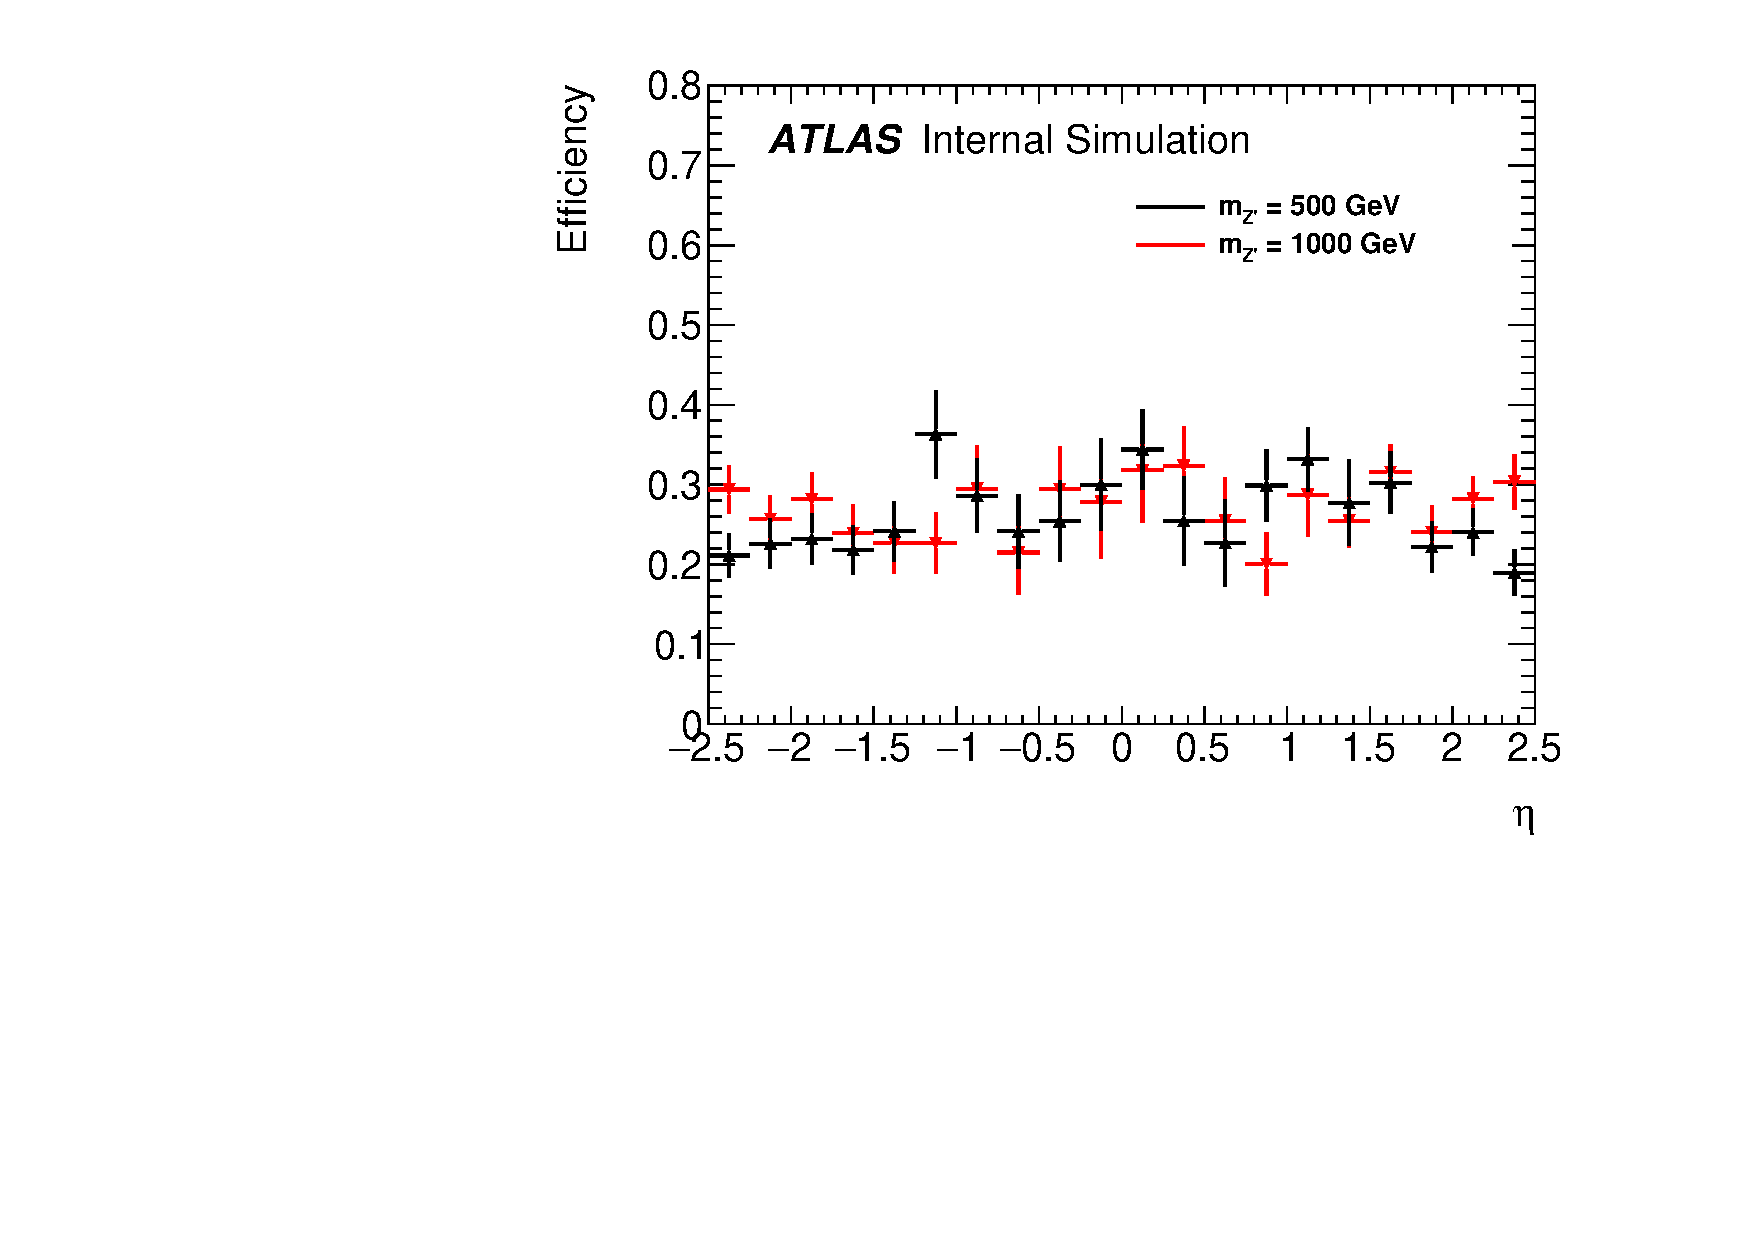
\includegraphics[width=0.49\textwidth]{figures/m_eff_dv_eta.pdf}}
    \subfloat[]{\label{subfig:vertex_dist_phi}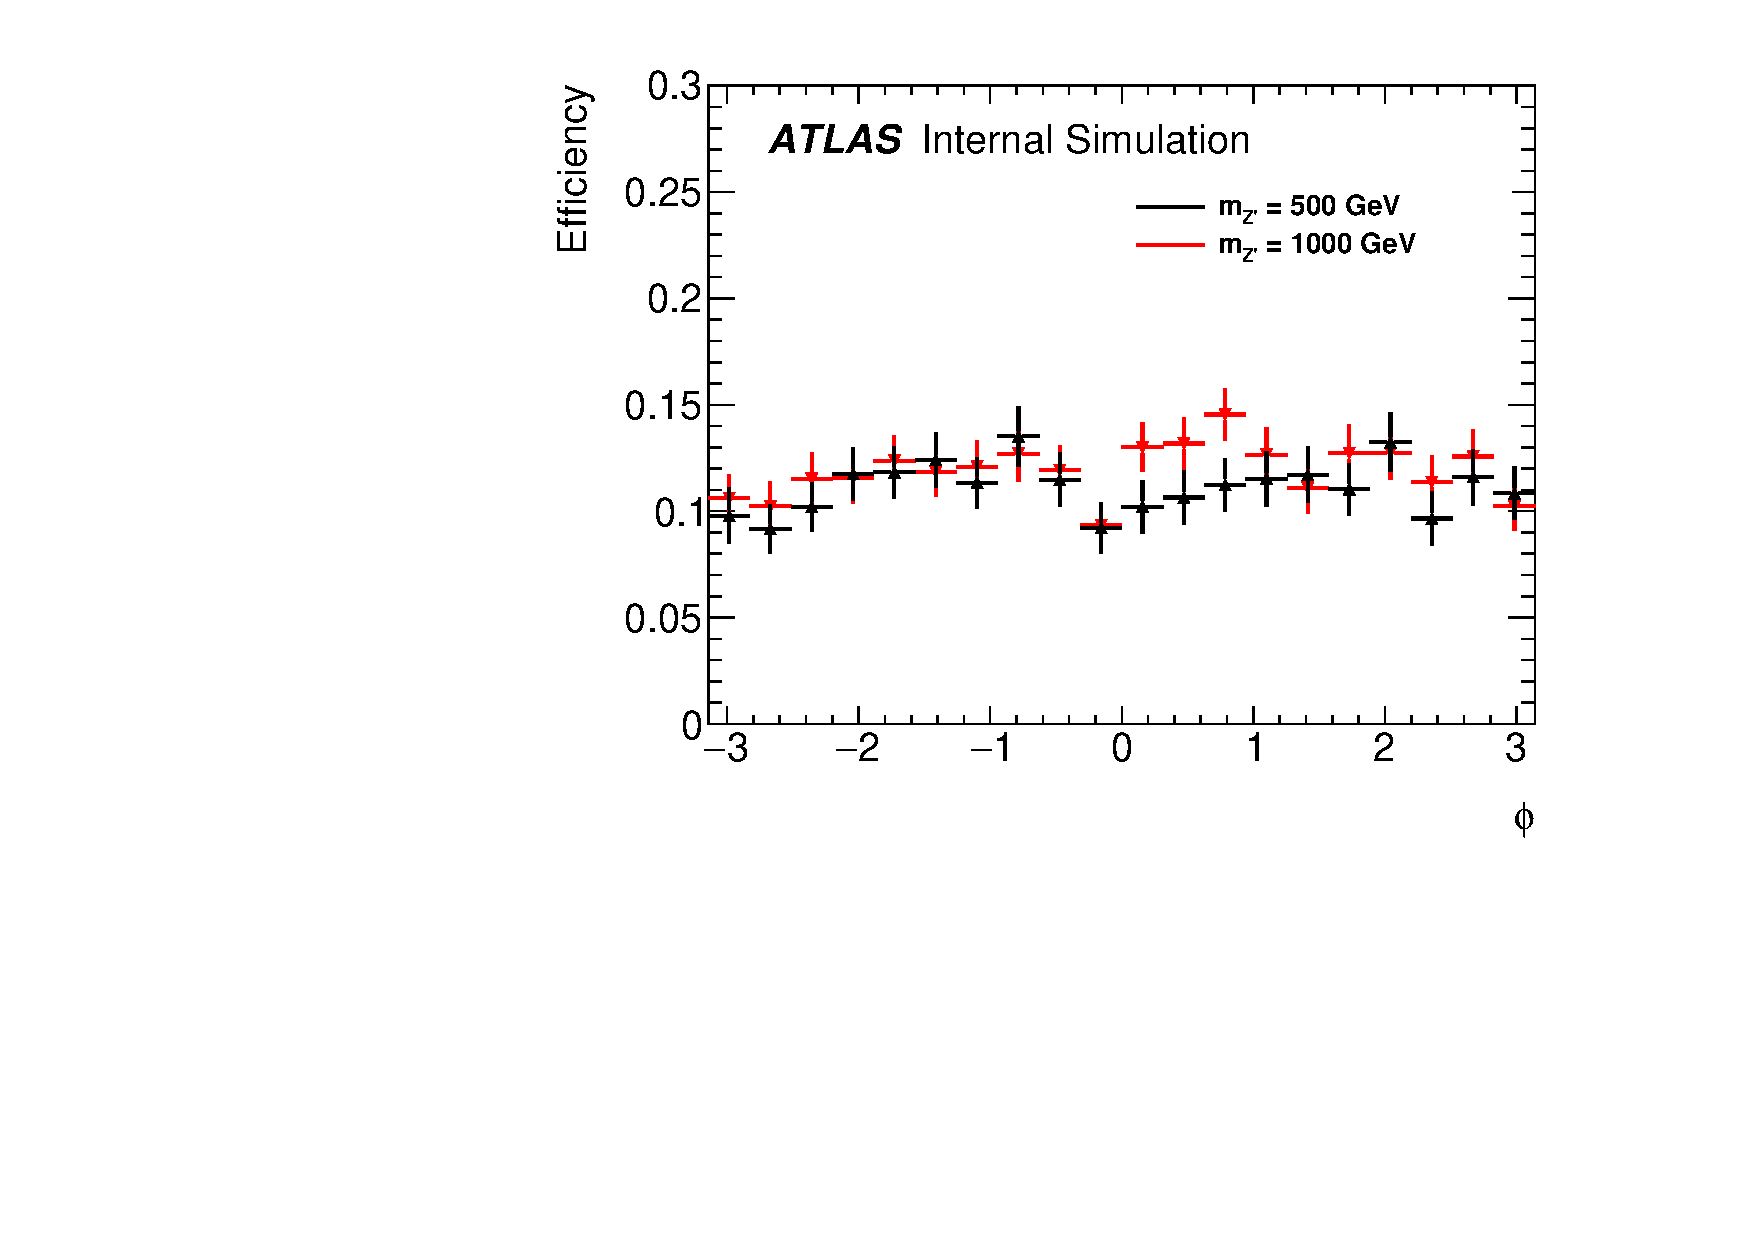
\includegraphics[width=0.49\textwidth]{figures/m_eff_dv_phi.pdf}}\\
    \subfloat[]{\label{subfig:vertex_dist_mu}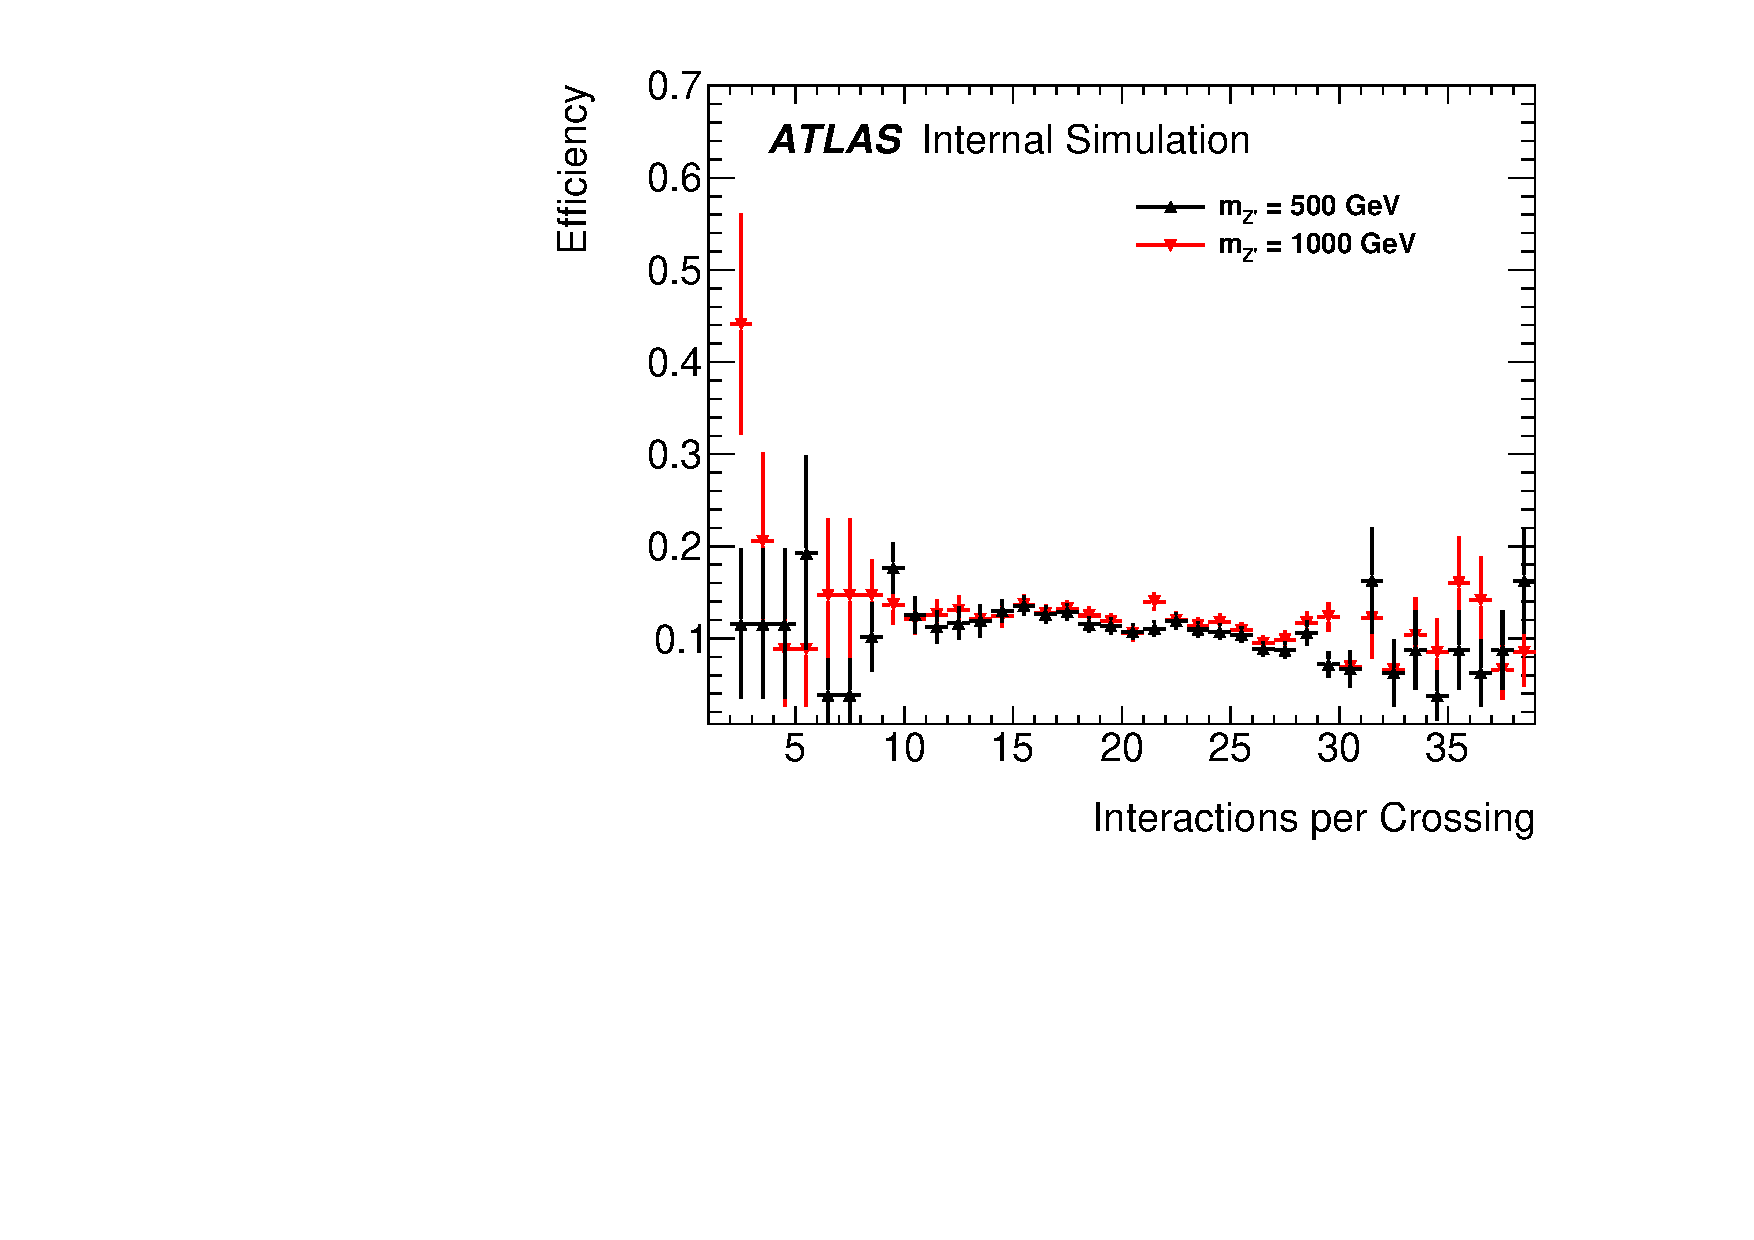
\includegraphics[width=0.49\textwidth]{figures/dv_eff_mu_zp.pdf}}
    \caption{Signal efficiency as a function of (a) $r$, (b) $z$, (c) $\eta$, (d) $\phi$, and (e) pile-up for the signal MC samples of $Z'\rightarrow \mumu$ with $m=$ 500, 1000 GeV for $c\tau=$ 100 mm.}
    \label{fig:signal_vertex_dist}
\end{figure}

The signal efficiency shows a dependence on vertex position which decreases at large $r$ and $z$ due to the minimum silicon hits requirement on tracks. The first (central) bins in $r$ ($z$) distributions have lower efficiency due to the minimum displacement requirement ($r_{\mathrm{DV}} > $ 2 mm) on secondary vertices. The $\eta$ distribution has an uniform efficiency of $\sim25\%$ for $|\eta|<$ 2.5. The $\phi$ distribution is uniform as expected. The pile-up distribution of the signal efficiency shows that the efficiency is reduced for high pile-up as expected.

The overall signal efficiency for the signal samples are shown in Table~\ref{table:signal_eff}. The signal efficiency is 6.0-12.2\% for mass above 500 GeV, but the efficiency is reduced for lower $Z'$ mass due to minimum $p_{T}$ thresholds on the leptons, especially for the samples with $m_{Z'}=100~\si{\GeV}$. The samples with shorter lifetime tend to have higher signal efficiency as expected. 

\begin{table}[!htb]
  \centering
  \begin{tabular}{ c c @{\hspace{1cm}} c @{\hspace{1cm}} c @{\hspace{1cm}} c }
    \hline
    \hline
    $m_{Z'}$ (GeV) & $c\tau$ (mm)    &$\mu\mu$ ($\%$)     & $ee$ ($\%$)     & $e\mu$ ($\%$)     \\
    \hline
    100			   &  100    & 0.46~$\pm$0.05 	& 0.07~$\pm$0.02	&  0.10~$\pm$0.02  \\
    100			   &  250    & 0.35~$\pm$0.04 	& 0.07~$\pm$0.02	&  0.08~$\pm$0.02  \\
    100			   &  500    & 0.20~$\pm$0.03 	& 0.05~$\pm$0.02	&  0.07~$\pm$0.02  \\
    250			   &  100    & 7.70~$\pm$0.19 	& 6.44~$\pm$0.17	&  3.10~$\pm$0.12  \\
    250			   &  250    & 7.12~$\pm$0.18 	& 5.59~$\pm$0.16	&  2.81~$\pm$0.12  \\
    250			   &  500    & 5.25~$\pm$0.16 	& 3.59~$\pm$0.13	&  2.19~$\pm$0.10  \\
    500			   &  100    & 9.67~$\pm$0.21 	& 8.16~$\pm$0.19	&  8.97~$\pm$0.21  \\
    500			   &  250    & 9.02~$\pm$0.20 	& 7.62~$\pm$0.19	&  8.25~$\pm$0.19  \\
    500			   &  500    & 7.00~$\pm$0.18 	& 5.96~$\pm$0.17	&  6.01~$\pm$0.17  \\
    750			   &  100    &10.23~$\pm$0.21	& 9.48~$\pm$0.21	& 11.45~$\pm$0.23  \\
    750			   &  250    &10.65~$\pm$0.22	& 8.94~$\pm$0.20	& 10.47~$\pm$0.22  \\
    750			   &  500    & 7.91~$\pm$0.19 	& 6.84~$\pm$0.18	&  7.89~$\pm$0.19  \\
    1000	           &  100    &10.43~$\pm$0.22	& 9.89~$\pm$0.21	& 11.86~$\pm$0.24  \\
    1000	           &  250    &11.11~$\pm$0.22	&10.15~$\pm$0.21	& 12.21~$\pm$0.23  \\
    1000	           &  500    & 9.26~$\pm$0.20 	& 7.97~$\pm$0.20	&  9.17~$\pm$0.21  \\
    \hline
    \hline
  \end{tabular}
  \caption{Overall signal efficiency of the signal samples. Statistical uncertainties are shown.}
  \label{table:signal_eff}
\end{table}




\subsection{Efficiency Map}
\label{sec:efficiency_map}
Signal efficiency for each mass and lifetime of long-lived $Z'$ sample is presented as a function of $p_{T}$ and $|\eta|$ of $Z'$. Because any neutral, LLP decaying to a dilepton pair can be characterized by mass, lifetime, $p_{T}$, and $\eta$ of the LLP, these efficiency maps can be used for other BSM searches such as searching for long-lived neutralino in the context of SUSY R-parity violating theory.

Representative efficiency maps are shown in Figure~\ref{fig:signal_eff_map} using the signal MC samples of $Z' \rightarrow \mu\mu, ee, e\mu$ with $m=$ 500, 1000 GeV and $c\tau=$ 100 mm. The overall signal efficiency is $\sim$10\%, but the efficiencies in the central region ($|\eta| < $ 2.5) are much higher. Efficiency maps of other signal samples are available in Appendix~\ref{app:signal_efficiency_map}.

\begin{figure}[!htb]
    \centering
    \subfloat[$Z'\rightarrow \mu\mu$, $m=500$ GeV]{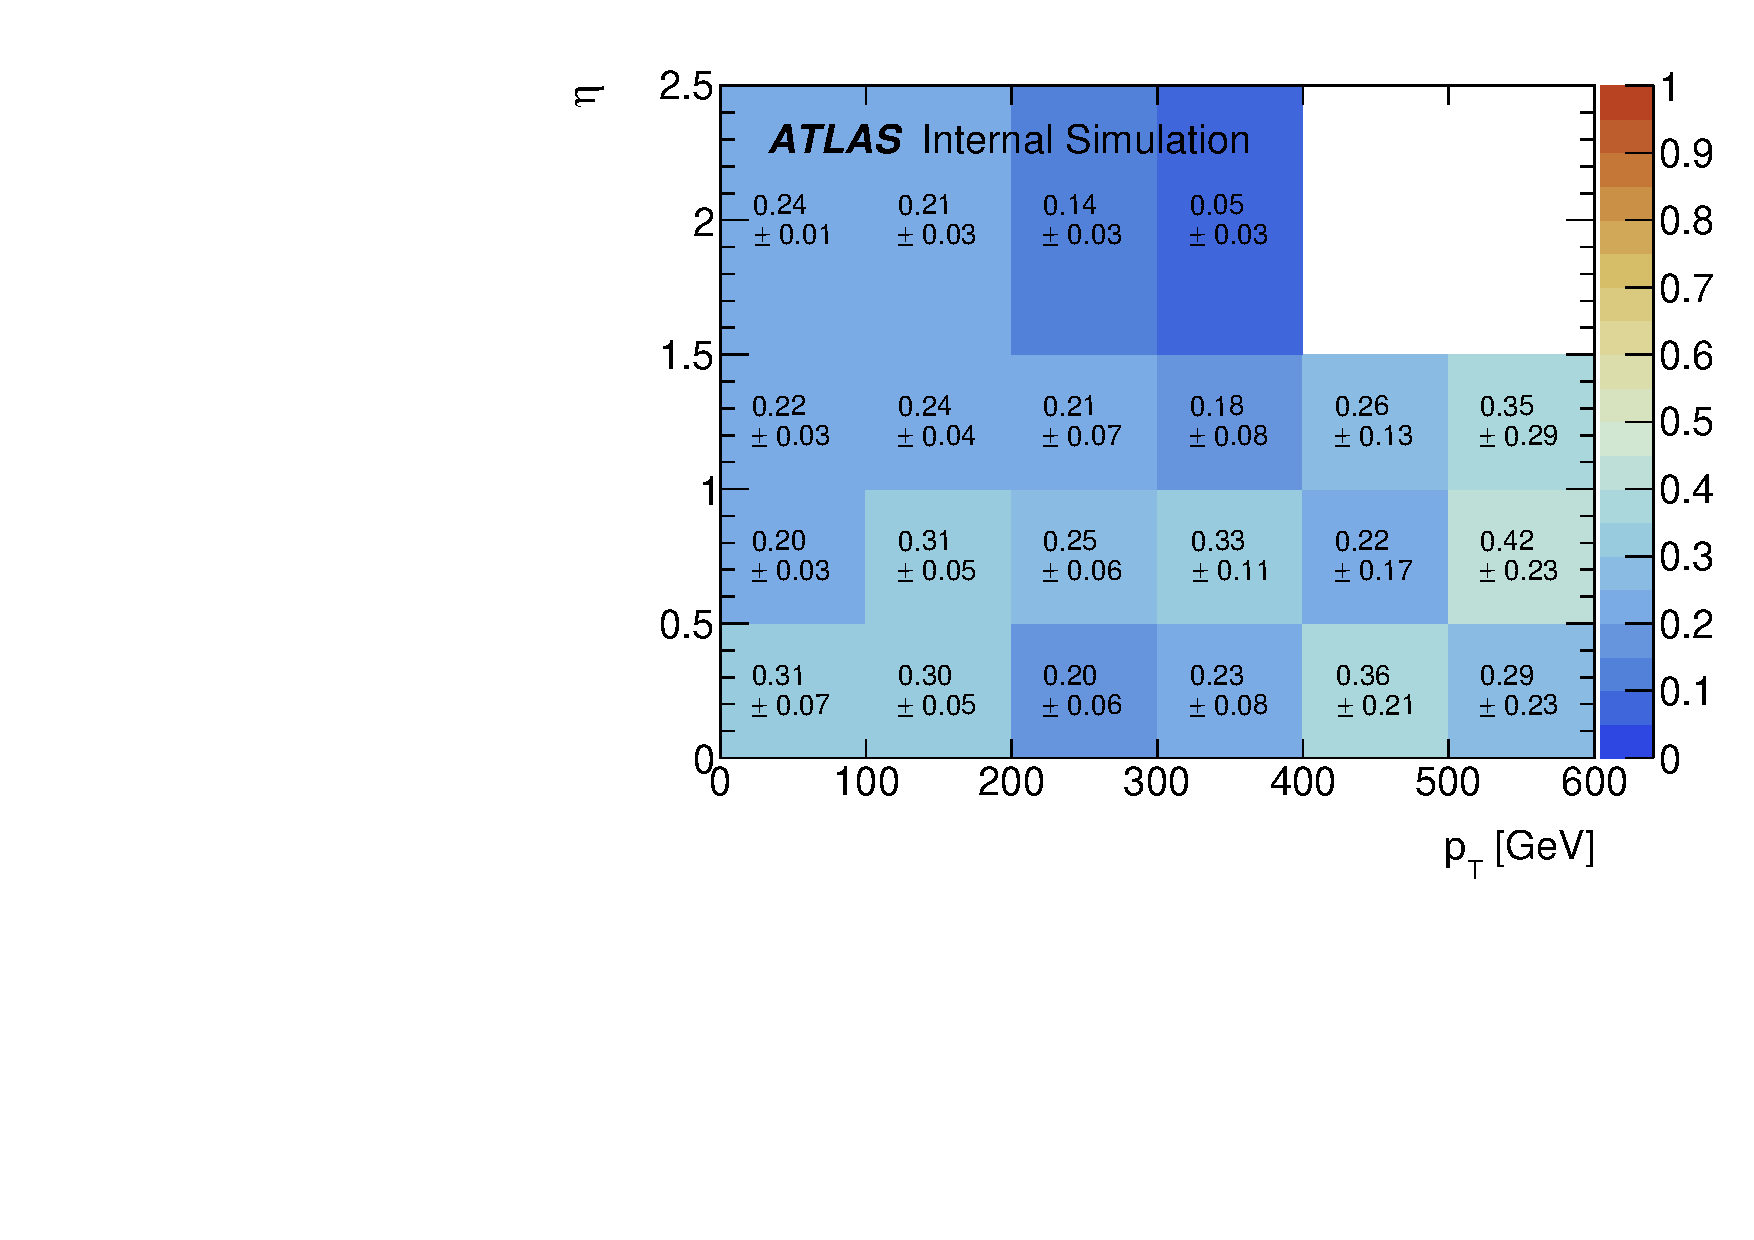
\includegraphics[width=0.50\textwidth]{figures/EfficiencyMap/eff_map_mumu_m500t100.pdf}}
    \subfloat[$Z'\rightarrow \mu\mu$, $m=1000$ GeV]{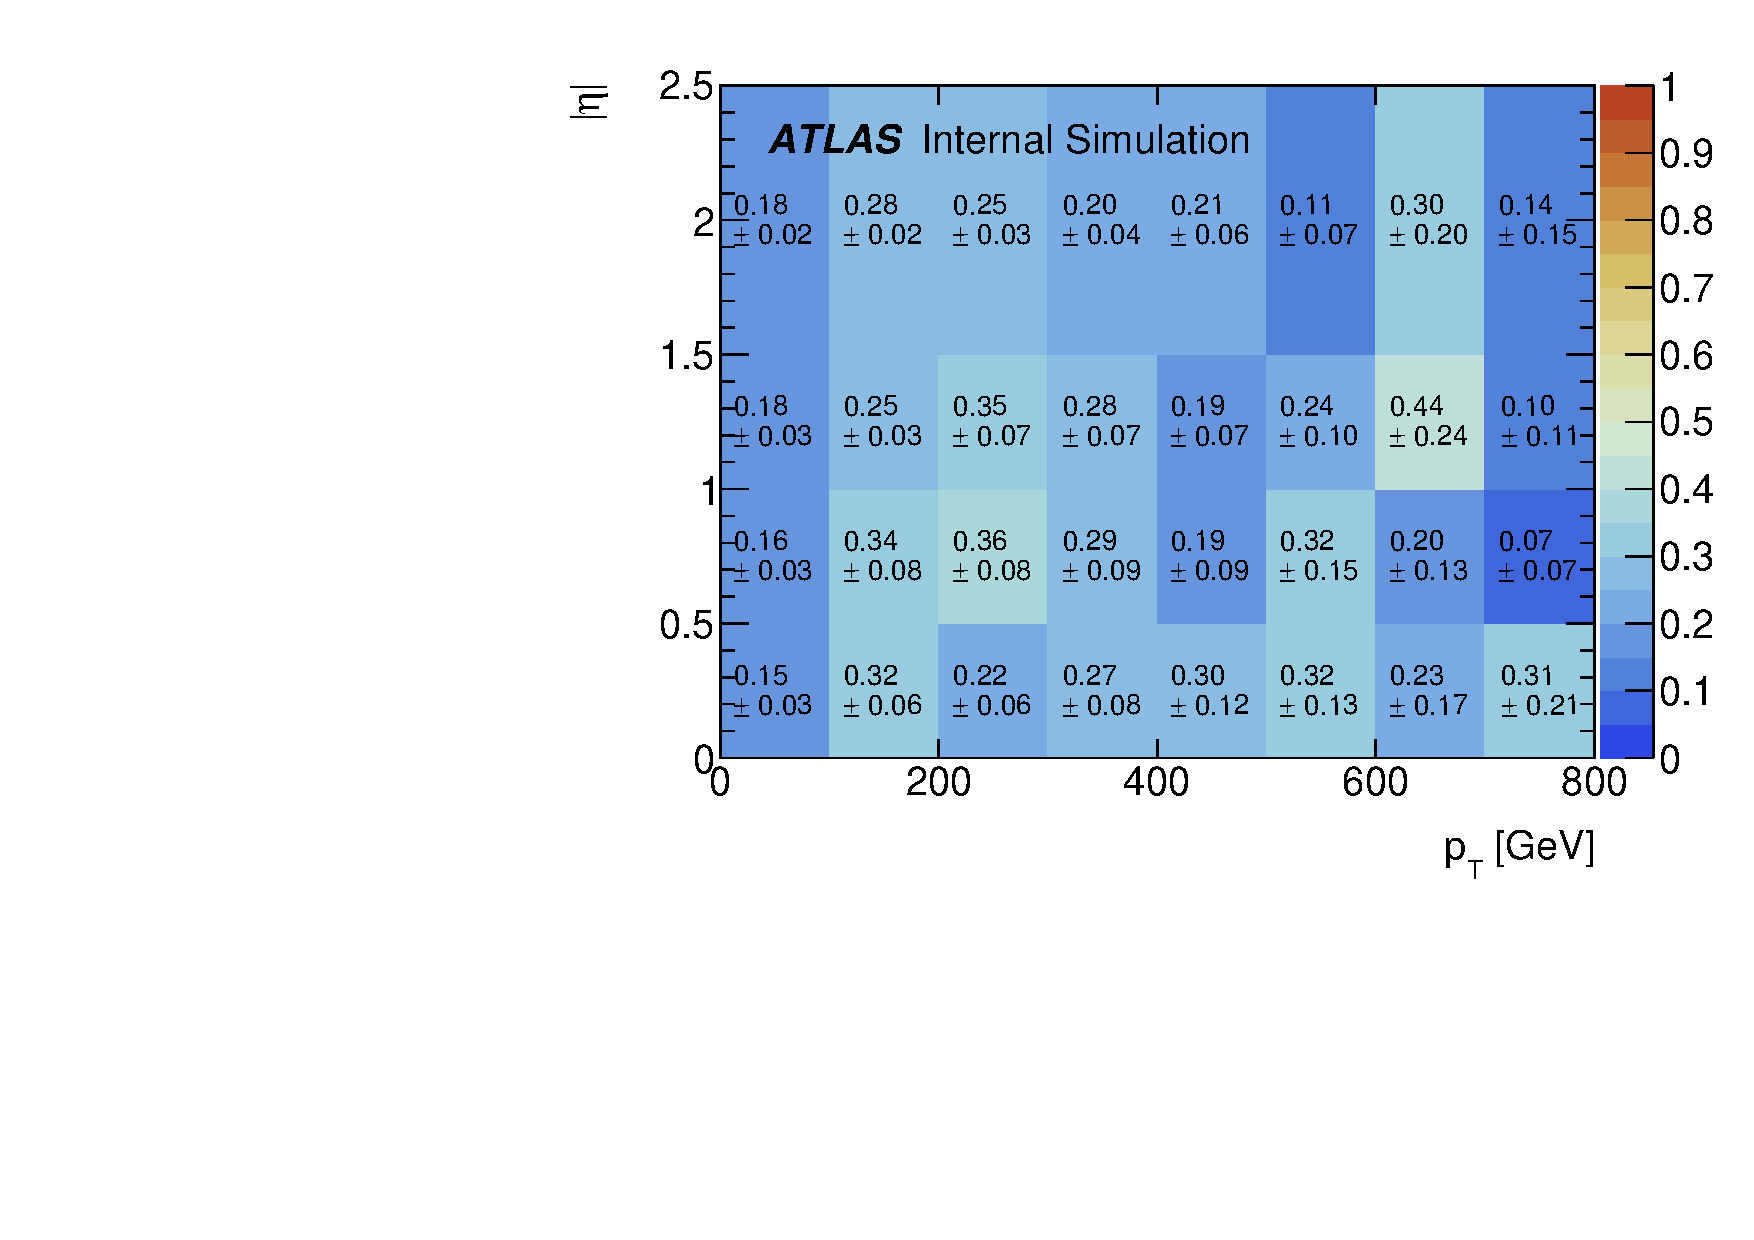
\includegraphics[width=0.50\textwidth]{figures/EfficiencyMap/eff_map_mumu_m1000t100.pdf}} \\
    \subfloat[$Z'\rightarrow ee$, $m=500$ GeV]{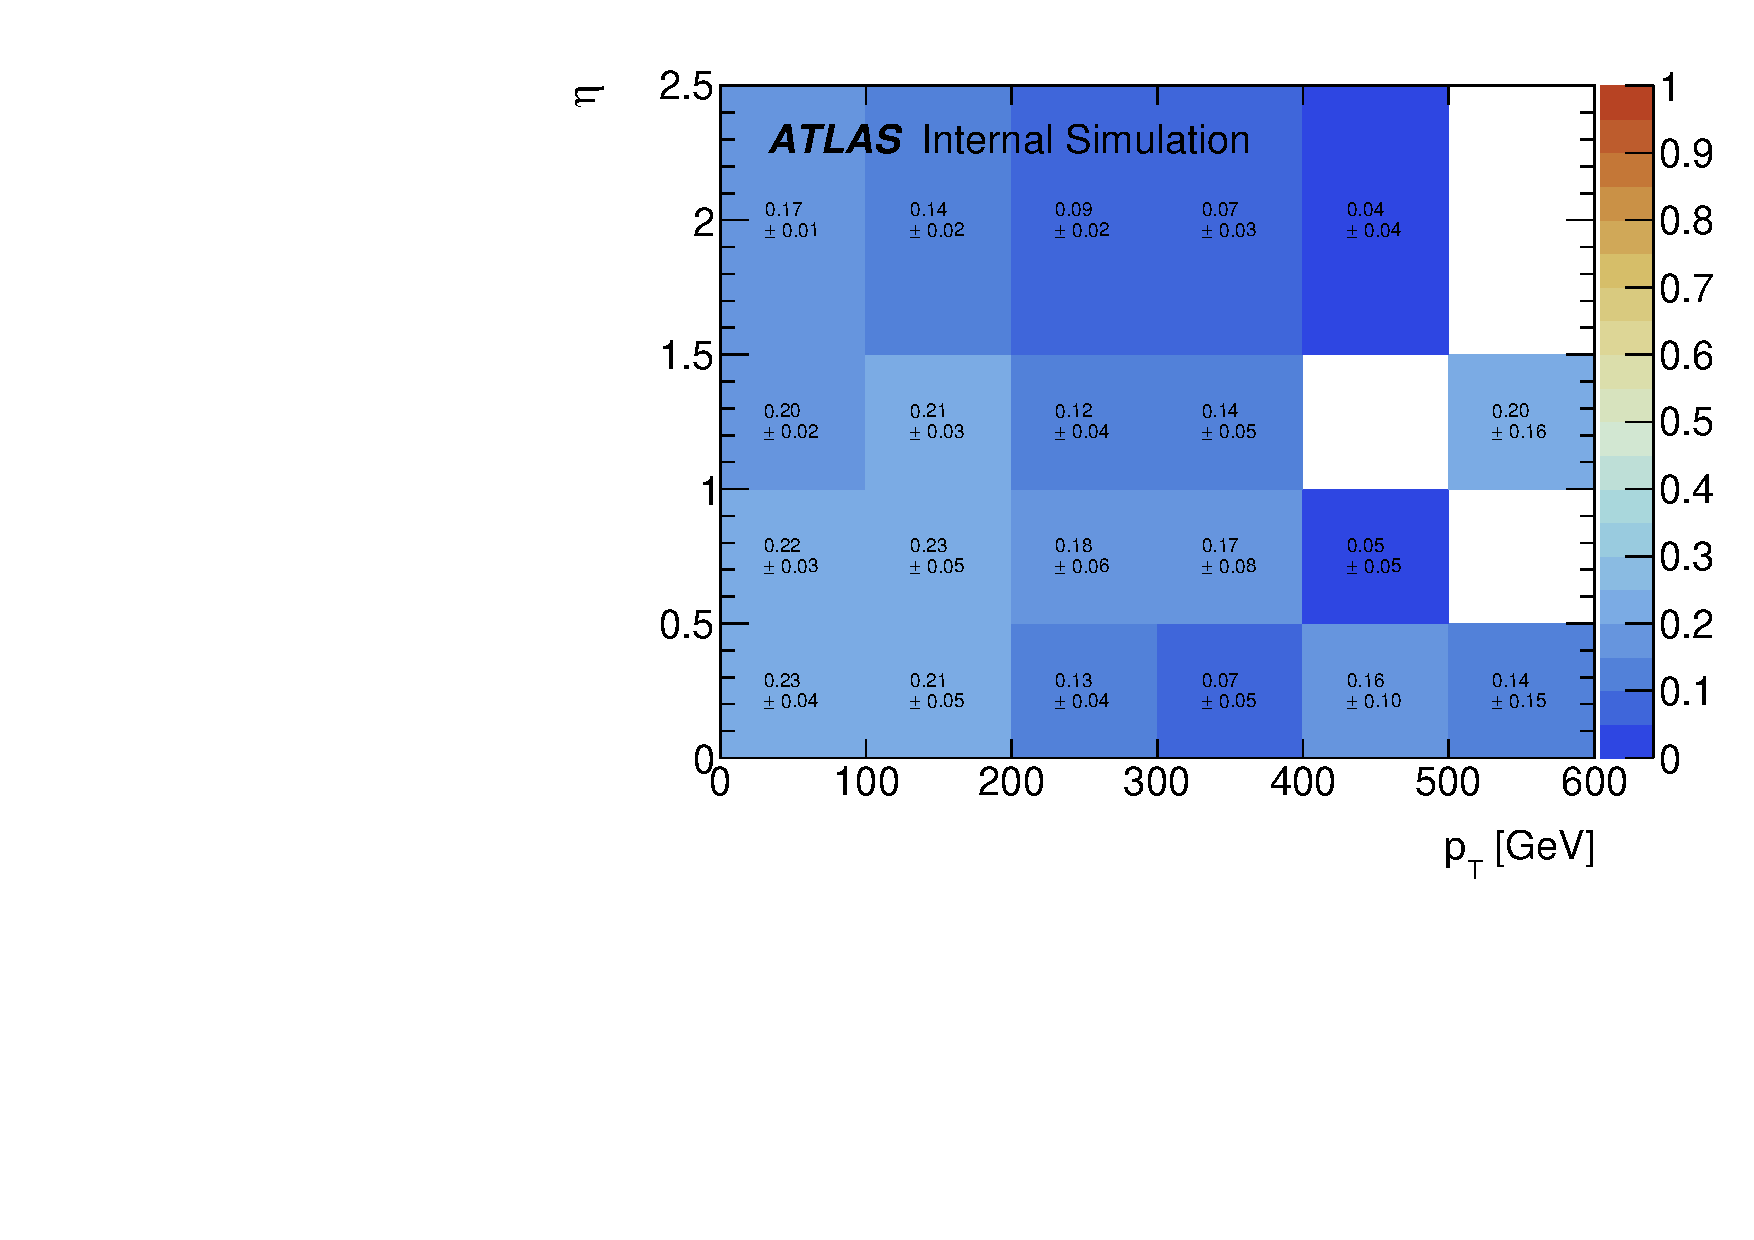
\includegraphics[width=0.50\textwidth]{figures/EfficiencyMap/eff_map_ee_m500t100.pdf}}
    \subfloat[$Z'\rightarrow ee$, $m=1000$ GeV]{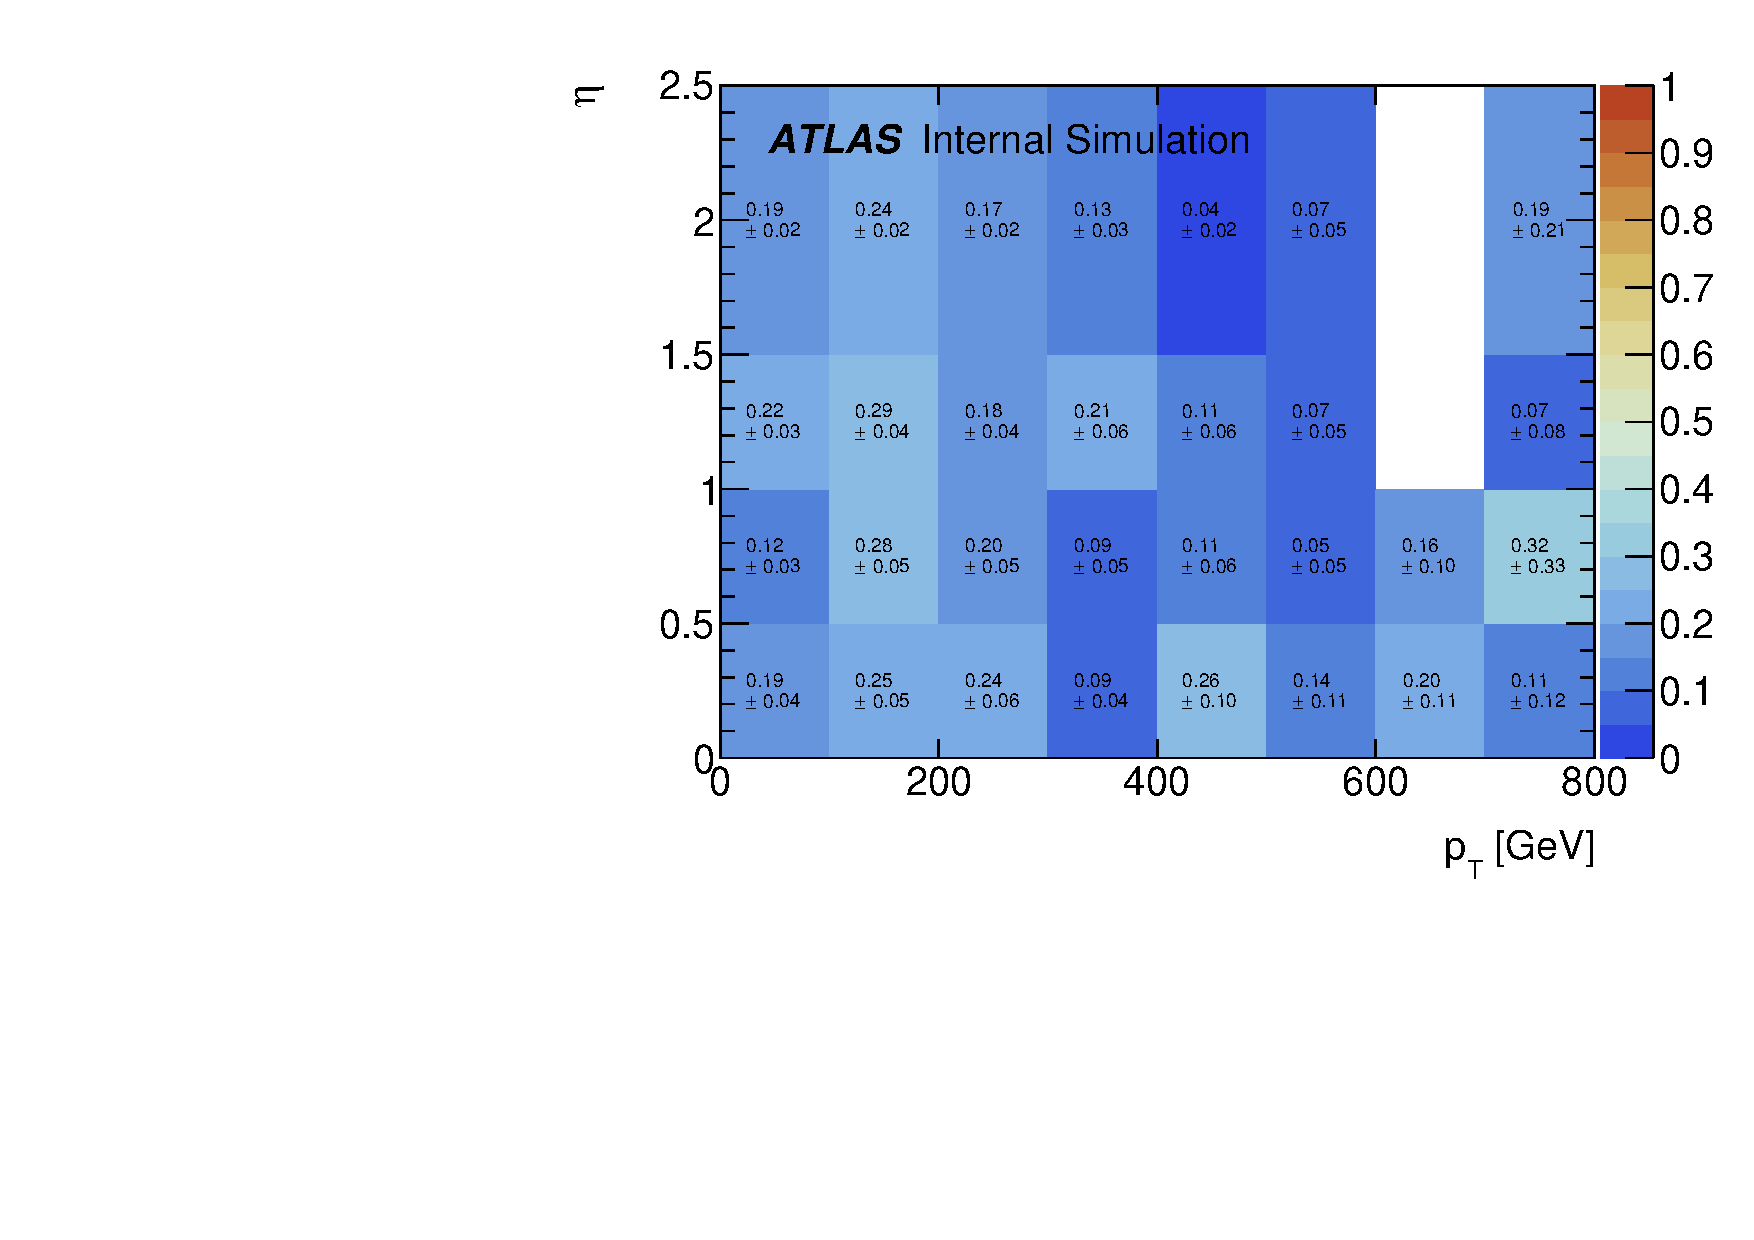
\includegraphics[width=0.50\textwidth]{figures/EfficiencyMap/eff_map_ee_m1000t100.pdf}} \\
    \subfloat[$Z'\rightarrow e\mu$, $m=500$ GeV]{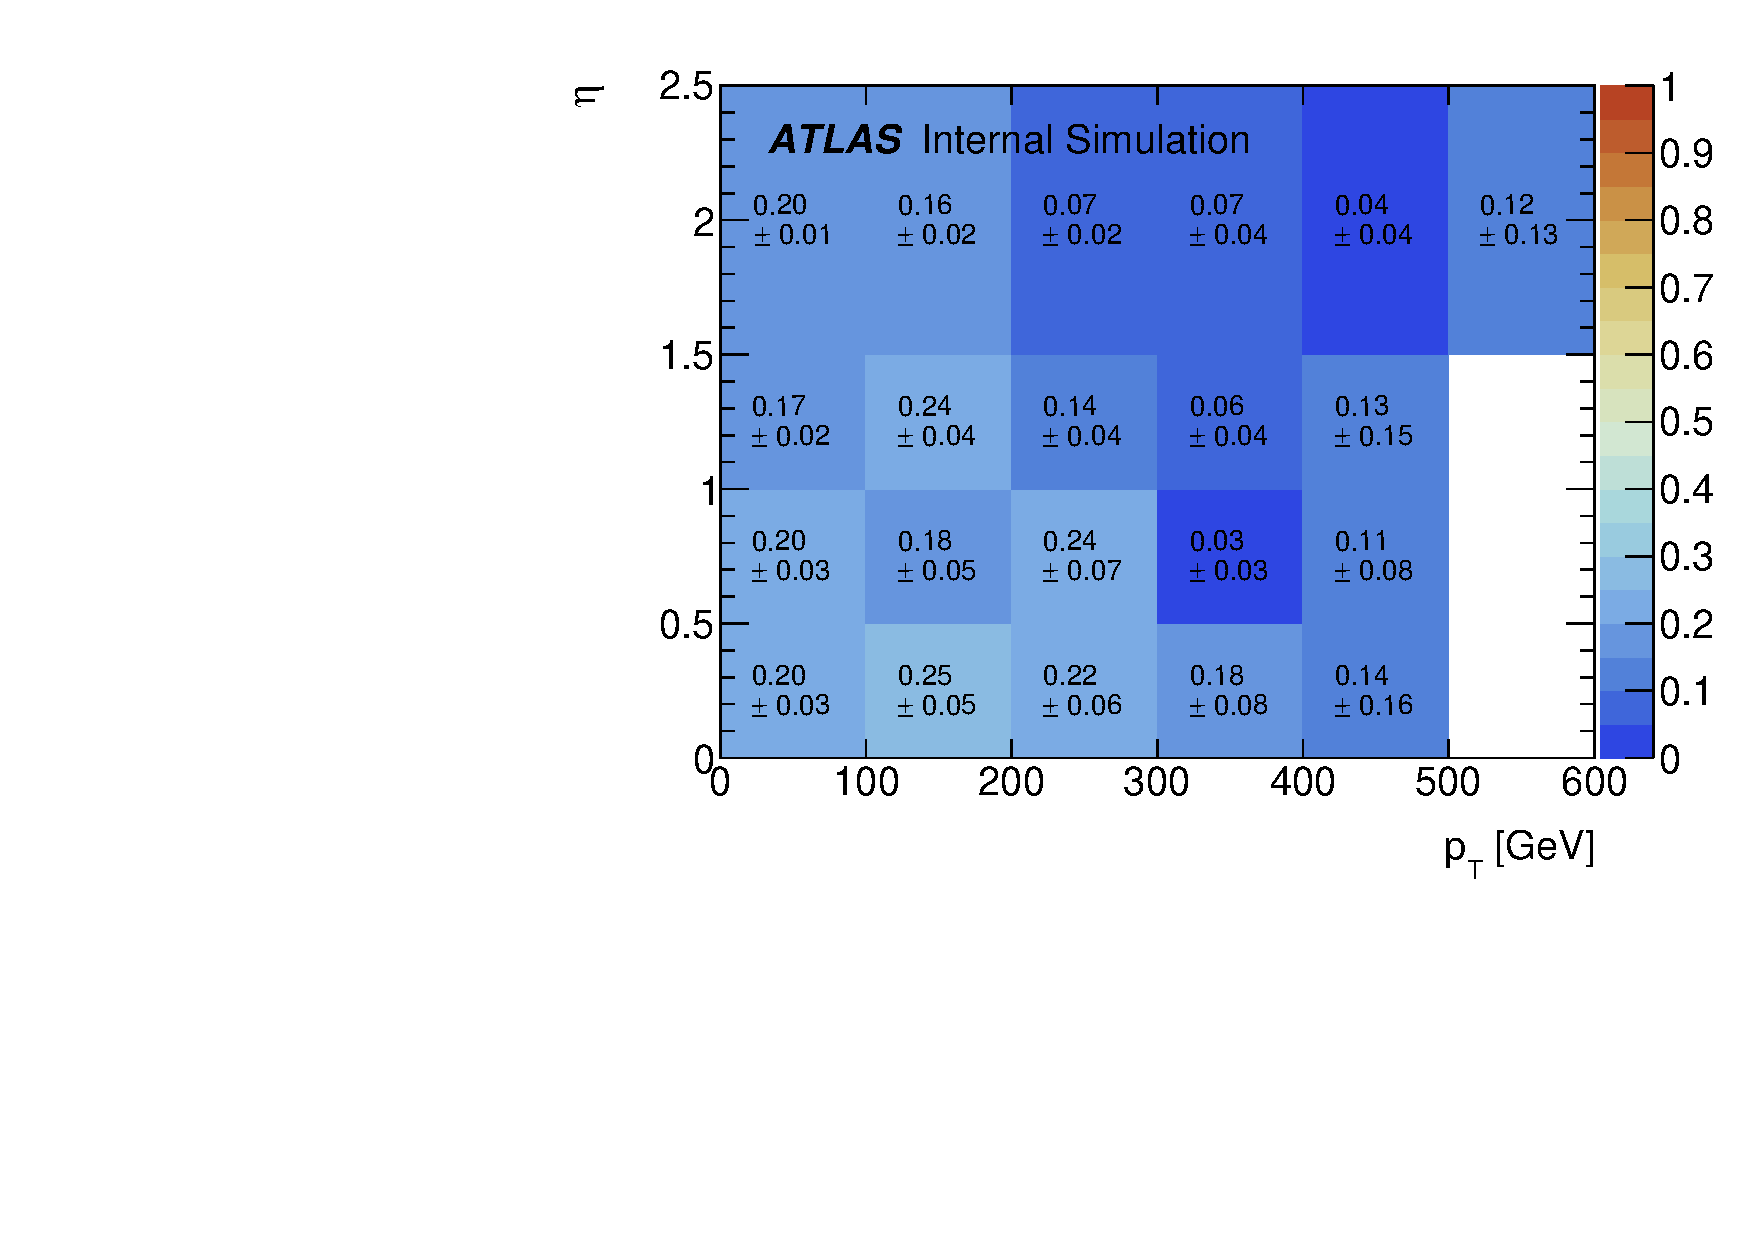
\includegraphics[width=0.50\textwidth]{figures/EfficiencyMap/eff_map_emu_m500t100.pdf}}
    \subfloat[$Z'\rightarrow e\mu$, $m=1000$ GeV]{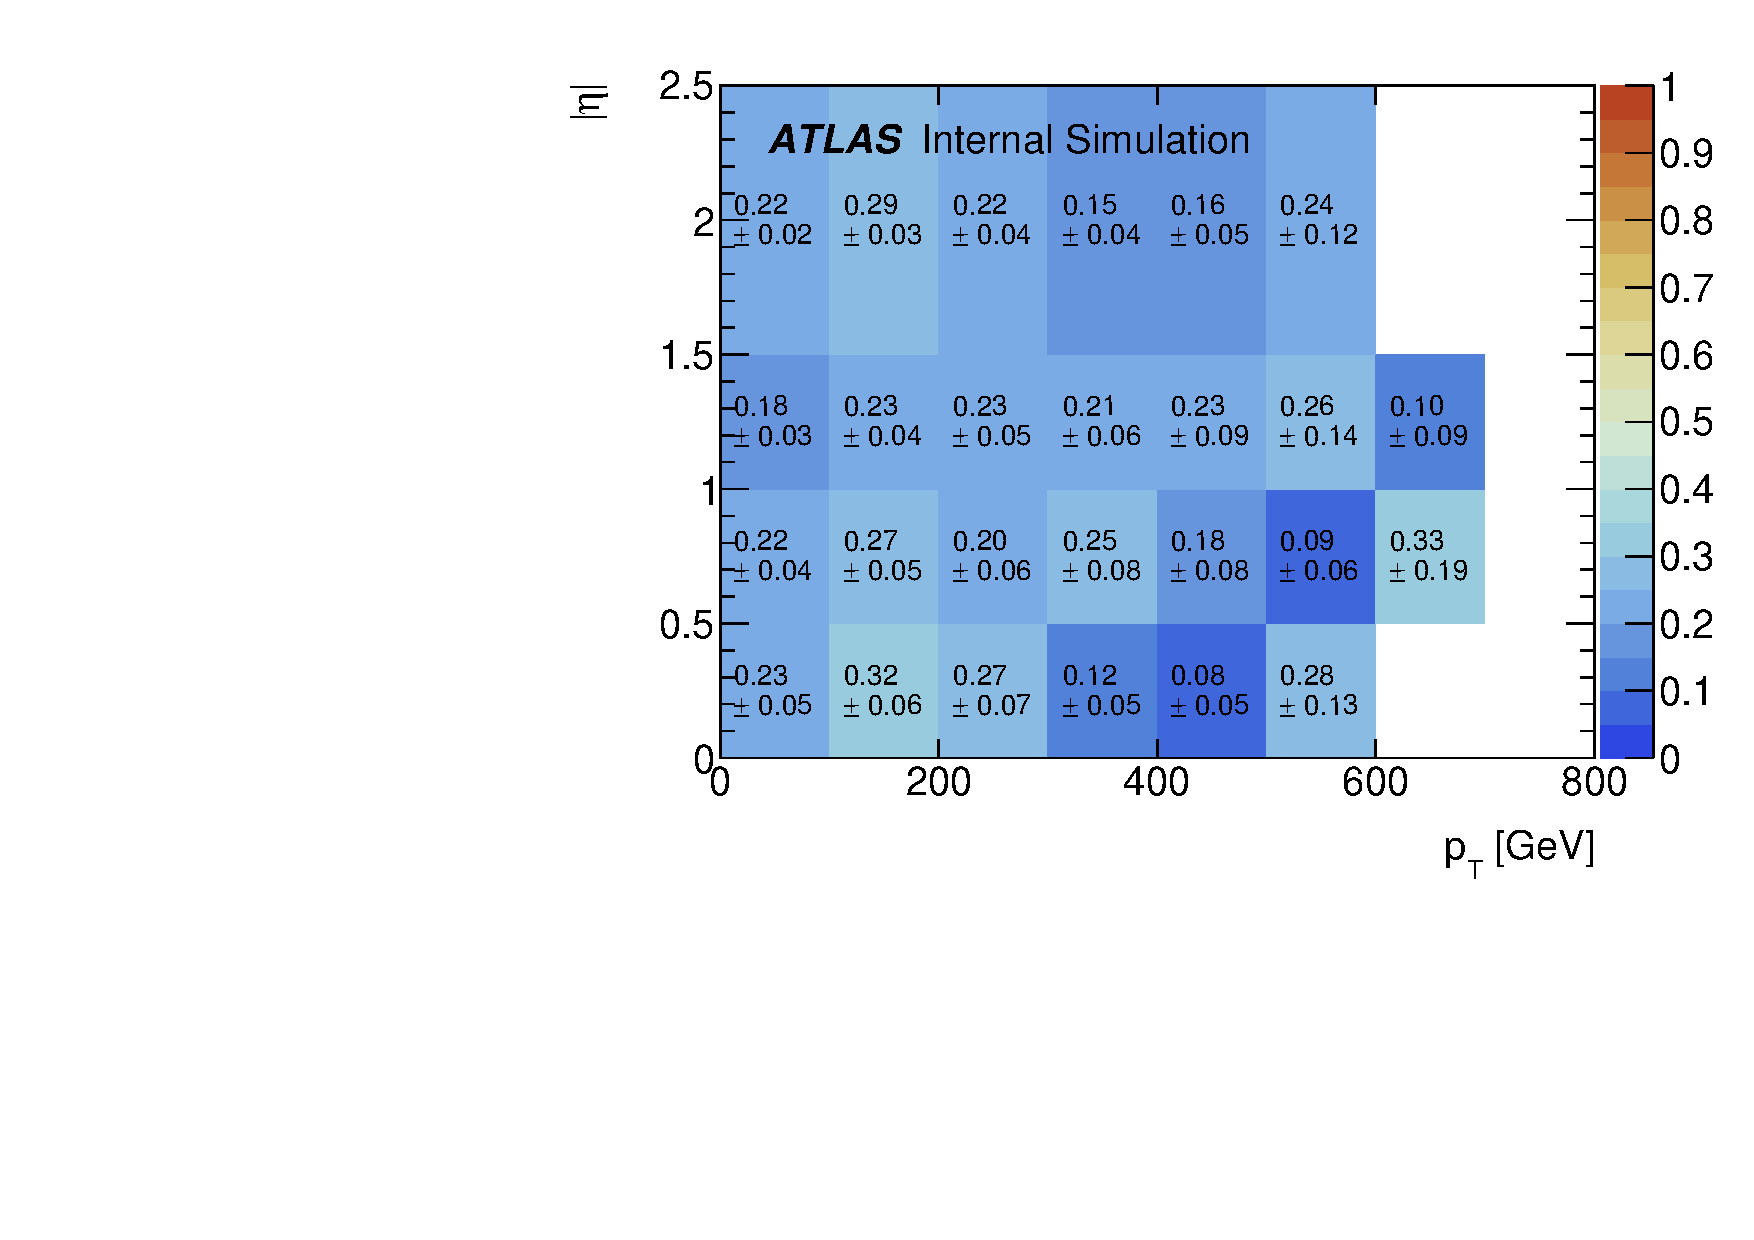
\includegraphics[width=0.50\textwidth]{figures/EfficiencyMap/eff_map_emu_m1000t100.pdf}}
    \caption{Signal efficiency maps of the signal MC sample of $Z' \rightarrow \mumu$ with (a) $m=500$ and (b) $m=1000$ GeV for $c\tau=$ 100 mm. The corresponding efficiency maps for $Z' \rightarrow \ee, \emu$ is shown in (c)$-$(f).}
    \label{fig:signal_eff_map}
\end{figure}







